% Opciones del tipo de documento
\documentclass[oneside,openright,titlepage,numbers=noenddot,openany,headinclude,footinclude=true,
cleardoublepage=empty,abstractoff,BCOR=5mm,paper=a4,fontsize=12pt,main=spanish]{scrreprt}

% Paquetes de latex que se cargan al inicio. Cubren la entrada de
% texto, gráficos, código fuente y símbolos.
\usepackage[utf8]{inputenc}
\usepackage[T1]{fontenc}
\usepackage{fixltx2e}
\usepackage{graphicx} % Inclusión de imágenes.
%\usepackage{grffile}  % Distintos formatos para imágenes.
%\usepackage{longtable} % Tablas multipágina.
%\usepackage{wrapfig} % Coloca texto alrededor de una figura.
\usepackage{rotating}
\usepackage[normalem]{ulem}
\usepackage{amsmath}
\usepackage{textcomp}
\usepackage{amssymb}
\usepackage{capt-of}
\usepackage[colorlinks=true]{hyperref}
%\usepackage{tikz} % Diagramas conmutativos.
\usepackage{minted} % Código fuente.
%\usepackage{natbib}
\usepackage[backend=bibtex8]{biblatex}
\addbibresource{bibliografia.bib}

%\usepackage[nonumberlist]{glossaries}

\usepackage{appendix}
\usepackage{caption}

\usepackage{adjustbox}
\usepackage[table]{xcolor}

\usepackage{fontawesome}

\usepackage{pbox}

\usepackage{pdfpages}



% Plantilla classicthesis
\usepackage[beramono,eulerchapternumbers,linedheaders,parts,a5paper,dottedtoc,
manychapters,pdfspacing]{classicthesis}

% Geometría y espaciado de párrafos.
\setcounter{secnumdepth}{0}
\usepackage{enumitem}
\setitemize{noitemsep,topsep=0pt,parsep=0pt,partopsep=0pt}
\setlist[enumerate]{topsep=0pt,itemsep=-1ex,partopsep=1ex,parsep=1ex}
\usepackage[top=1in, bottom=1.5in, left=1in, right=1in]{geometry}
\setlength\itemsep{0em}
\setlength{\parindent}{0pt}
\usepackage{parskip}

% Profundidad de la tabla de contenidos.
\setcounter{secnumdepth}{3}

% Usa el paquete minted para mostrar trozos de código.
% Pueden seleccionarse el lenguaje apropiado y el estilo del código.
\usepackage{minted}
\usemintedstyle{colorful}
\setminted{fontsize=\small}
\setminted[php]{linenos=false,fontsize=\small}
\renewcommand{\theFancyVerbLine}{\sffamily\textcolor[rgb]{0.5,0.5,1.0}{\oldstylenums{\arabic{FancyVerbLine}}}}

% Archivos de configuración.
%%------------------------
% Bibliotecas para matemáticas de latex
%------------------------
\usepackage{amsthm}
\usepackage{amsmath}
\usepackage{tikz}
\usepackage{tikz-cd}
\usetikzlibrary{shapes,fit}
\usepackage{bussproofs}
\EnableBpAbbreviations{}
\usepackage{mathtools}
\usepackage{scalerel}
\usepackage{stmaryrd}

%------------------------
% Estilos para los teoremas
%------------------------
\theoremstyle{plain}
\newtheorem{theorem}{Teorema}
\newtheorem{proposition}{Proposición}
\newtheorem{lemma}{Lema}
\newtheorem{corollary}{Corolario}
\theoremstyle{definition}
\newtheorem{definition}{Definición}
\newtheorem{proofs}{Demostración}
\theoremstyle{remark}
\newtheorem{remark}{Comentario}
\newtheorem{exampleth}{Ejemplo}

\begingroup\makeatletter\@for\theoremstyle:=definition,remark,plain\do{\expandafter\g@addto@macro\csname th@\theoremstyle\endcsname{\addtolength\thm@preskip\parskip}}\endgroup

%------------------------
% Macros
% ------------------------

% Aquí pueden añadirse abreviaturas para comandos de latex
% frequentemente usados.
\newcommand*\diff{\mathop{}\!\mathrm{d}}  % En macros.tex se almacenan las opciones y comandos para escribir matemáticas.
% ****************************************************************************************************
% classicthesis-config.tex 
% formerly known as loadpackages.sty, classicthesis-ldpkg.sty, and classicthesis-preamble.sty 
% Use it at the beginning of your ClassicThesis.tex, or as a LaTeX Preamble 
% in your ClassicThesis.{tex,lyx} with % ****************************************************************************************************
% classicthesis-config.tex 
% formerly known as loadpackages.sty, classicthesis-ldpkg.sty, and classicthesis-preamble.sty 
% Use it at the beginning of your ClassicThesis.tex, or as a LaTeX Preamble 
% in your ClassicThesis.{tex,lyx} with % ****************************************************************************************************
% classicthesis-config.tex 
% formerly known as loadpackages.sty, classicthesis-ldpkg.sty, and classicthesis-preamble.sty 
% Use it at the beginning of your ClassicThesis.tex, or as a LaTeX Preamble 
% in your ClassicThesis.{tex,lyx} with \input{classicthesis-config}
% ****************************************************************************************************  
% If you like the classicthesis, then I would appreciate a postcard. 
% My address can be found in the file ClassicThesis.pdf. A collection 
% of the postcards I received so far is available online at 
% http://postcards.miede.de
% ****************************************************************************************************


% ****************************************************************************************************
% 0. Set the encoding of your files. UTF-8 is the only sensible encoding nowadays. If you can't read
% äöüßáéçèê∂åëæƒÏ€ then change the encoding setting in your editor, not the line below. If your editor
% does not support utf8 use another editor!
% ****************************************************************************************************
\PassOptionsToPackage{utf8x}{inputenc}
	\usepackage{inputenc}

% ****************************************************************************************************
% 1. Configure classicthesis for your needs here, e.g., remove "drafting" below 
% in order to deactivate the time-stamp on the pages
% ****************************************************************************************************
\PassOptionsToPackage{eulerchapternumbers,listings,drafting,%
		pdfspacing,%floatperchapter,%linedheaders,%
                subfig,beramono,eulermath,parts,dottedtoc}{classicthesis}                                        
% ********************************************************************
% Available options for classicthesis.sty 
% (see ClassicThesis.pdf for more information):
% drafting
% parts nochapters linedheaders
% eulerchapternumbers beramono eulermath pdfspacing minionprospacing
% tocaligned dottedtoc manychapters
% listings floatperchapter subfig
% ********************************************************************

% ****************************************************************************************************
% 2. Personal data and user ad-hoc commands
% ****************************************************************************************************
\newcommand{\myTitle}{A Classic Thesis Style\xspace}
\newcommand{\mySubtitle}{An Homage to The Elements of Typographic Style\xspace}
\newcommand{\myDegree}{Doktor-Ingenieur (Dr.-Ing.)\xspace}
\newcommand{\myName}{André Miede\xspace}
\newcommand{\myProf}{Put name here\xspace}
\newcommand{\myOtherProf}{Put name here\xspace}
\newcommand{\mySupervisor}{Put name here\xspace}
\newcommand{\myFaculty}{Put data here\xspace}
\newcommand{\myDepartment}{Put data here\xspace}
\newcommand{\myUni}{Put data here\xspace}
\newcommand{\myLocation}{Saarbrücken\xspace}
\newcommand{\myTime}{September 2015\xspace}
%\newcommand{\myVersion}{version 4.2\xspace}

% ********************************************************************
% Setup, finetuning, and useful commands
% ********************************************************************
\newcounter{dummy} % necessary for correct hyperlinks (to index, bib, etc.)
\newlength{\abcd} % for ab..z string length calculation
\providecommand{\mLyX}{L\kern-.1667em\lower.25em\hbox{Y}\kern-.125emX\@}
\newcommand{\ie}{i.\,e.}
\newcommand{\Ie}{I.\,e.}
\newcommand{\eg}{e.\,g.}
\newcommand{\Eg}{E.\,g.} 
% ****************************************************************************************************


% ****************************************************************************************************
% 3. Loading some handy packages
% ****************************************************************************************************
% ******************************************************************** 
% Packages with options that might require adjustments
% ******************************************************************** 
%\PassOptionsToPackage{ngerman,american}{babel}   % change this to your language(s)
% Spanish languages need extra options in order to work with this template
% \PassOptionsToPackage{es-lcroman,spanish}{babel}
\usepackage[main=spanish]{babel}

%\usepackage{csquotes}
% \PassOptionsToPackage{%
%     %backend=biber, %instead of bibtex
% 	backend=bibtex8,bibencoding=ascii,%
% 	language=auto,%
% 	style=alpha,%
%     %style=authoryear-comp, % Author 1999, 2010
%     %bibstyle=authoryear,dashed=false, % dashed: substitute rep. author with ---
%     sorting=nyt, % name, year, title
%     maxbibnames=10, % default: 3, et al.
%     %backref=true,%
%     natbib=true % natbib compatibility mode (\citep and \citet still work)
% }{biblatex}
%     \usepackage{biblatex}

% \PassOptionsToPackage{fleqn}{amsmath}       % math environments and more by the AMS 
%     \usepackage{amsmath}

% ******************************************************************** 
% General useful packages
% ******************************************************************** 
\PassOptionsToPackage{T1}{fontenc} % T2A for cyrillics
    \usepackage{fontenc}     
\usepackage{textcomp} % fix warning with missing font shapes
\usepackage{scrhack} % fix warnings when using KOMA with listings package          
\usepackage{xspace} % to get the spacing after macros right  
\usepackage{mparhack} % get marginpar right
\usepackage{fixltx2e} % fixes some LaTeX stuff --> since 2015 in the LaTeX kernel (see below)
%\usepackage[latest]{latexrelease} % will be used once available in more distributions (ISSUE #107)
\PassOptionsToPackage{printonlyused,smaller}{acronym} 
    \usepackage{acronym} % nice macros for handling all acronyms in the thesis
    %\renewcommand{\bflabel}[1]{{#1}\hfill} % fix the list of acronyms --> no longer working
    %\renewcommand*{\acsfont}[1]{\textsc{#1}} 
    \renewcommand*{\aclabelfont}[1]{\acsfont{#1}}
% ****************************************************************************************************


% ****************************************************************************************************
% 4. Setup floats: tables, (sub)figures, and captions
% ****************************************************************************************************
\usepackage{tabularx} % better tables
    \setlength{\extrarowheight}{3pt} % increase table row height
\newcommand{\tableheadline}[1]{\multicolumn{1}{c}{\spacedlowsmallcaps{#1}}}
\newcommand{\myfloatalign}{\centering} % to be used with each float for alignment
\usepackage{caption}
% Thanks to cgnieder and Claus Lahiri
% http://tex.stackexchange.com/questions/69349/spacedlowsmallcaps-in-caption-label
% [REMOVED DUE TO OTHER PROBLEMS, SEE ISSUE #82]    
%\DeclareCaptionLabelFormat{smallcaps}{\bothIfFirst{#1}{~}\MakeTextLowercase{\textsc{#2}}}
%\captionsetup{font=small,labelformat=smallcaps} % format=hang,
\captionsetup{font=small} % format=hang,
\usepackage{subfig}  
% ****************************************************************************************************


% ****************************************************************************************************
% 5. Setup code listings
% ****************************************************************************************************
% \usepackage{listings} 
% %\lstset{emph={trueIndex,root},emphstyle=\color{BlueViolet}}%\underbar} % for special keywords
% \lstset{language={Haskell},morekeywords={PassOptionsToPackage,selectlanguage},keywordstyle=\color{RoyalBlue},basicstyle=\small\ttfamily,commentstyle=\color{Green}\ttfamily,stringstyle=\rmfamily,numbers=none,numberstyle=\scriptsize,stepnumber=5,numbersep=8pt,showstringspaces=false,breaklines=true,belowcaptionskip=.75\baselineskip} 
% ****************************************************************************************************             


% ****************************************************************************************************
% 6. PDFLaTeX, hyperreferences and citation backreferences
% ****************************************************************************************************
% ********************************************************************
% Using PDFLaTeX
% ********************************************************************
\PassOptionsToPackage{pdftex,hyperfootnotes=false,pdfpagelabels}{hyperref}
    \usepackage{hyperref}  % backref linktocpage pagebackref
\pdfcompresslevel=9
\pdfadjustspacing=1 
\PassOptionsToPackage{pdftex}{graphicx}
    \usepackage{graphicx} 
 

% ********************************************************************
% Hyperreferences
% ********************************************************************
\hypersetup{%
    %draft, % = no hyperlinking at all (useful in b/w printouts)
    colorlinks=true, linktocpage=true, pdfstartpage=3, pdfstartview=FitV,%
    % uncomment the following line if you want to have black links (e.g., for printing)
    %colorlinks=false, linktocpage=false, pdfstartpage=3, pdfstartview=FitV, pdfborder={0 0 0},%
    breaklinks=true, pdfpagemode=UseNone, pageanchor=true, pdfpagemode=UseOutlines,%
    plainpages=false, bookmarksnumbered, bookmarksopen=true, bookmarksopenlevel=1,%
    hypertexnames=true, pdfhighlight=/O,%nesting=true,%frenchlinks,%
    urlcolor=webbrown, linkcolor=RoyalBlue, citecolor=webgreen, %pagecolor=RoyalBlue,%
    %urlcolor=Black, linkcolor=Black, citecolor=Black, %pagecolor=Black,%
    pdftitle={\myTitle},%
    pdfauthor={\textcopyright\ \myName, \myUni, \myFaculty},%
    pdfsubject={},%
    pdfkeywords={},%
    pdfcreator={pdfLaTeX},%
    pdfproducer={LaTeX with hyperref and classicthesis}%
}   

% ********************************************************************
% Setup autoreferences
% ********************************************************************
% There are some issues regarding autorefnames
% http://www.ureader.de/msg/136221647.aspx
% http://www.tex.ac.uk/cgi-bin/texfaq2html?label=latexwords
% you have to redefine the makros for the 
% language you use, e.g., american, ngerman
% (as chosen when loading babel/AtBeginDocument)
% ********************************************************************
\makeatletter
\@ifpackageloaded{babel}%
    {%
       \addto\extrasamerican{%
			\renewcommand*{\figureautorefname}{Figure}%
			\renewcommand*{\tableautorefname}{Table}%
			\renewcommand*{\partautorefname}{Part}%
			\renewcommand*{\chapterautorefname}{Chapter}%
			\renewcommand*{\sectionautorefname}{Section}%
			\renewcommand*{\subsectionautorefname}{Section}%
			\renewcommand*{\subsubsectionautorefname}{Section}%     
                }%
       \addto\extrasngerman{% 
			\renewcommand*{\paragraphautorefname}{Absatz}%
			\renewcommand*{\subparagraphautorefname}{Unterabsatz}%
			\renewcommand*{\footnoteautorefname}{Fu\"snote}%
			\renewcommand*{\FancyVerbLineautorefname}{Zeile}%
			\renewcommand*{\theoremautorefname}{Theorem}%
			\renewcommand*{\appendixautorefname}{Anhang}%
			\renewcommand*{\equationautorefname}{Gleichung}%        
			\renewcommand*{\itemautorefname}{Punkt}%
                }%  
            % Fix to getting autorefs for subfigures right (thanks to Belinda Vogt for changing the definition)
            \providecommand{\subfigureautorefname}{\figureautorefname}%             
    }{\relax}
\makeatother


% ****************************************************************************************************
% 7. Last calls before the bar closes
% ****************************************************************************************************
% ********************************************************************
% Development Stuff
% ********************************************************************
\listfiles
%\PassOptionsToPackage{l2tabu,orthodox,abort}{nag}
%   \usepackage{nag}
%\PassOptionsToPackage{warning, all}{onlyamsmath}
%   \usepackage{onlyamsmath}

% ********************************************************************
% Last, but not least...
% ********************************************************************
\usepackage{classicthesis} 
% ****************************************************************************************************


% ****************************************************************************************************
% 8. Further adjustments (experimental)
% ****************************************************************************************************
% ********************************************************************
% Changing the text area
% ********************************************************************
%\linespread{1.05} % a bit more for Palatino
%\areaset[current]{312pt}{761pt} % 686 (factor 2.2) + 33 head + 42 head \the\footskip
%\setlength{\marginparwidth}{7em}%
%\setlength{\marginparsep}{2em}%

% ********************************************************************
% Using different fonts
% ********************************************************************
%\usepackage[oldstylenums]{kpfonts} % oldstyle notextcomp
%\usepackage[osf]{libertine}
%\usepackage[light,condensed,math]{iwona}
%\renewcommand{\sfdefault}{iwona}
%\usepackage{lmodern} % <-- no osf support :-(
%\usepackage{cfr-lm} % 
%\usepackage[urw-garamond]{mathdesign} <-- no osf support :-(
%\usepackage[default,osfigures]{opensans} % scale=0.95 
%\usepackage[sfdefault]{FiraSans}
% ****************************************************************************************************

% ****************************************************************************************************  
% If you like the classicthesis, then I would appreciate a postcard. 
% My address can be found in the file ClassicThesis.pdf. A collection 
% of the postcards I received so far is available online at 
% http://postcards.miede.de
% ****************************************************************************************************


% ****************************************************************************************************
% 0. Set the encoding of your files. UTF-8 is the only sensible encoding nowadays. If you can't read
% äöüßáéçèê∂åëæƒÏ€ then change the encoding setting in your editor, not the line below. If your editor
% does not support utf8 use another editor!
% ****************************************************************************************************
\PassOptionsToPackage{utf8x}{inputenc}
	\usepackage{inputenc}

% ****************************************************************************************************
% 1. Configure classicthesis for your needs here, e.g., remove "drafting" below 
% in order to deactivate the time-stamp on the pages
% ****************************************************************************************************
\PassOptionsToPackage{eulerchapternumbers,listings,drafting,%
		pdfspacing,%floatperchapter,%linedheaders,%
                subfig,beramono,eulermath,parts,dottedtoc}{classicthesis}                                        
% ********************************************************************
% Available options for classicthesis.sty 
% (see ClassicThesis.pdf for more information):
% drafting
% parts nochapters linedheaders
% eulerchapternumbers beramono eulermath pdfspacing minionprospacing
% tocaligned dottedtoc manychapters
% listings floatperchapter subfig
% ********************************************************************

% ****************************************************************************************************
% 2. Personal data and user ad-hoc commands
% ****************************************************************************************************
\newcommand{\myTitle}{A Classic Thesis Style\xspace}
\newcommand{\mySubtitle}{An Homage to The Elements of Typographic Style\xspace}
\newcommand{\myDegree}{Doktor-Ingenieur (Dr.-Ing.)\xspace}
\newcommand{\myName}{André Miede\xspace}
\newcommand{\myProf}{Put name here\xspace}
\newcommand{\myOtherProf}{Put name here\xspace}
\newcommand{\mySupervisor}{Put name here\xspace}
\newcommand{\myFaculty}{Put data here\xspace}
\newcommand{\myDepartment}{Put data here\xspace}
\newcommand{\myUni}{Put data here\xspace}
\newcommand{\myLocation}{Saarbrücken\xspace}
\newcommand{\myTime}{September 2015\xspace}
%\newcommand{\myVersion}{version 4.2\xspace}

% ********************************************************************
% Setup, finetuning, and useful commands
% ********************************************************************
\newcounter{dummy} % necessary for correct hyperlinks (to index, bib, etc.)
\newlength{\abcd} % for ab..z string length calculation
\providecommand{\mLyX}{L\kern-.1667em\lower.25em\hbox{Y}\kern-.125emX\@}
\newcommand{\ie}{i.\,e.}
\newcommand{\Ie}{I.\,e.}
\newcommand{\eg}{e.\,g.}
\newcommand{\Eg}{E.\,g.} 
% ****************************************************************************************************


% ****************************************************************************************************
% 3. Loading some handy packages
% ****************************************************************************************************
% ******************************************************************** 
% Packages with options that might require adjustments
% ******************************************************************** 
%\PassOptionsToPackage{ngerman,american}{babel}   % change this to your language(s)
% Spanish languages need extra options in order to work with this template
% \PassOptionsToPackage{es-lcroman,spanish}{babel}
\usepackage[main=spanish]{babel}

%\usepackage{csquotes}
% \PassOptionsToPackage{%
%     %backend=biber, %instead of bibtex
% 	backend=bibtex8,bibencoding=ascii,%
% 	language=auto,%
% 	style=alpha,%
%     %style=authoryear-comp, % Author 1999, 2010
%     %bibstyle=authoryear,dashed=false, % dashed: substitute rep. author with ---
%     sorting=nyt, % name, year, title
%     maxbibnames=10, % default: 3, et al.
%     %backref=true,%
%     natbib=true % natbib compatibility mode (\citep and \citet still work)
% }{biblatex}
%     \usepackage{biblatex}

% \PassOptionsToPackage{fleqn}{amsmath}       % math environments and more by the AMS 
%     \usepackage{amsmath}

% ******************************************************************** 
% General useful packages
% ******************************************************************** 
\PassOptionsToPackage{T1}{fontenc} % T2A for cyrillics
    \usepackage{fontenc}     
\usepackage{textcomp} % fix warning with missing font shapes
\usepackage{scrhack} % fix warnings when using KOMA with listings package          
\usepackage{xspace} % to get the spacing after macros right  
\usepackage{mparhack} % get marginpar right
\usepackage{fixltx2e} % fixes some LaTeX stuff --> since 2015 in the LaTeX kernel (see below)
%\usepackage[latest]{latexrelease} % will be used once available in more distributions (ISSUE #107)
\PassOptionsToPackage{printonlyused,smaller}{acronym} 
    \usepackage{acronym} % nice macros for handling all acronyms in the thesis
    %\renewcommand{\bflabel}[1]{{#1}\hfill} % fix the list of acronyms --> no longer working
    %\renewcommand*{\acsfont}[1]{\textsc{#1}} 
    \renewcommand*{\aclabelfont}[1]{\acsfont{#1}}
% ****************************************************************************************************


% ****************************************************************************************************
% 4. Setup floats: tables, (sub)figures, and captions
% ****************************************************************************************************
\usepackage{tabularx} % better tables
    \setlength{\extrarowheight}{3pt} % increase table row height
\newcommand{\tableheadline}[1]{\multicolumn{1}{c}{\spacedlowsmallcaps{#1}}}
\newcommand{\myfloatalign}{\centering} % to be used with each float for alignment
\usepackage{caption}
% Thanks to cgnieder and Claus Lahiri
% http://tex.stackexchange.com/questions/69349/spacedlowsmallcaps-in-caption-label
% [REMOVED DUE TO OTHER PROBLEMS, SEE ISSUE #82]    
%\DeclareCaptionLabelFormat{smallcaps}{\bothIfFirst{#1}{~}\MakeTextLowercase{\textsc{#2}}}
%\captionsetup{font=small,labelformat=smallcaps} % format=hang,
\captionsetup{font=small} % format=hang,
\usepackage{subfig}  
% ****************************************************************************************************


% ****************************************************************************************************
% 5. Setup code listings
% ****************************************************************************************************
% \usepackage{listings} 
% %\lstset{emph={trueIndex,root},emphstyle=\color{BlueViolet}}%\underbar} % for special keywords
% \lstset{language={Haskell},morekeywords={PassOptionsToPackage,selectlanguage},keywordstyle=\color{RoyalBlue},basicstyle=\small\ttfamily,commentstyle=\color{Green}\ttfamily,stringstyle=\rmfamily,numbers=none,numberstyle=\scriptsize,stepnumber=5,numbersep=8pt,showstringspaces=false,breaklines=true,belowcaptionskip=.75\baselineskip} 
% ****************************************************************************************************             


% ****************************************************************************************************
% 6. PDFLaTeX, hyperreferences and citation backreferences
% ****************************************************************************************************
% ********************************************************************
% Using PDFLaTeX
% ********************************************************************
\PassOptionsToPackage{pdftex,hyperfootnotes=false,pdfpagelabels}{hyperref}
    \usepackage{hyperref}  % backref linktocpage pagebackref
\pdfcompresslevel=9
\pdfadjustspacing=1 
\PassOptionsToPackage{pdftex}{graphicx}
    \usepackage{graphicx} 
 

% ********************************************************************
% Hyperreferences
% ********************************************************************
\hypersetup{%
    %draft, % = no hyperlinking at all (useful in b/w printouts)
    colorlinks=true, linktocpage=true, pdfstartpage=3, pdfstartview=FitV,%
    % uncomment the following line if you want to have black links (e.g., for printing)
    %colorlinks=false, linktocpage=false, pdfstartpage=3, pdfstartview=FitV, pdfborder={0 0 0},%
    breaklinks=true, pdfpagemode=UseNone, pageanchor=true, pdfpagemode=UseOutlines,%
    plainpages=false, bookmarksnumbered, bookmarksopen=true, bookmarksopenlevel=1,%
    hypertexnames=true, pdfhighlight=/O,%nesting=true,%frenchlinks,%
    urlcolor=webbrown, linkcolor=RoyalBlue, citecolor=webgreen, %pagecolor=RoyalBlue,%
    %urlcolor=Black, linkcolor=Black, citecolor=Black, %pagecolor=Black,%
    pdftitle={\myTitle},%
    pdfauthor={\textcopyright\ \myName, \myUni, \myFaculty},%
    pdfsubject={},%
    pdfkeywords={},%
    pdfcreator={pdfLaTeX},%
    pdfproducer={LaTeX with hyperref and classicthesis}%
}   

% ********************************************************************
% Setup autoreferences
% ********************************************************************
% There are some issues regarding autorefnames
% http://www.ureader.de/msg/136221647.aspx
% http://www.tex.ac.uk/cgi-bin/texfaq2html?label=latexwords
% you have to redefine the makros for the 
% language you use, e.g., american, ngerman
% (as chosen when loading babel/AtBeginDocument)
% ********************************************************************
\makeatletter
\@ifpackageloaded{babel}%
    {%
       \addto\extrasamerican{%
			\renewcommand*{\figureautorefname}{Figure}%
			\renewcommand*{\tableautorefname}{Table}%
			\renewcommand*{\partautorefname}{Part}%
			\renewcommand*{\chapterautorefname}{Chapter}%
			\renewcommand*{\sectionautorefname}{Section}%
			\renewcommand*{\subsectionautorefname}{Section}%
			\renewcommand*{\subsubsectionautorefname}{Section}%     
                }%
       \addto\extrasngerman{% 
			\renewcommand*{\paragraphautorefname}{Absatz}%
			\renewcommand*{\subparagraphautorefname}{Unterabsatz}%
			\renewcommand*{\footnoteautorefname}{Fu\"snote}%
			\renewcommand*{\FancyVerbLineautorefname}{Zeile}%
			\renewcommand*{\theoremautorefname}{Theorem}%
			\renewcommand*{\appendixautorefname}{Anhang}%
			\renewcommand*{\equationautorefname}{Gleichung}%        
			\renewcommand*{\itemautorefname}{Punkt}%
                }%  
            % Fix to getting autorefs for subfigures right (thanks to Belinda Vogt for changing the definition)
            \providecommand{\subfigureautorefname}{\figureautorefname}%             
    }{\relax}
\makeatother


% ****************************************************************************************************
% 7. Last calls before the bar closes
% ****************************************************************************************************
% ********************************************************************
% Development Stuff
% ********************************************************************
\listfiles
%\PassOptionsToPackage{l2tabu,orthodox,abort}{nag}
%   \usepackage{nag}
%\PassOptionsToPackage{warning, all}{onlyamsmath}
%   \usepackage{onlyamsmath}

% ********************************************************************
% Last, but not least...
% ********************************************************************
\usepackage{classicthesis} 
% ****************************************************************************************************


% ****************************************************************************************************
% 8. Further adjustments (experimental)
% ****************************************************************************************************
% ********************************************************************
% Changing the text area
% ********************************************************************
%\linespread{1.05} % a bit more for Palatino
%\areaset[current]{312pt}{761pt} % 686 (factor 2.2) + 33 head + 42 head \the\footskip
%\setlength{\marginparwidth}{7em}%
%\setlength{\marginparsep}{2em}%

% ********************************************************************
% Using different fonts
% ********************************************************************
%\usepackage[oldstylenums]{kpfonts} % oldstyle notextcomp
%\usepackage[osf]{libertine}
%\usepackage[light,condensed,math]{iwona}
%\renewcommand{\sfdefault}{iwona}
%\usepackage{lmodern} % <-- no osf support :-(
%\usepackage{cfr-lm} % 
%\usepackage[urw-garamond]{mathdesign} <-- no osf support :-(
%\usepackage[default,osfigures]{opensans} % scale=0.95 
%\usepackage[sfdefault]{FiraSans}
% ****************************************************************************************************

% ****************************************************************************************************  
% If you like the classicthesis, then I would appreciate a postcard. 
% My address can be found in the file ClassicThesis.pdf. A collection 
% of the postcards I received so far is available online at 
% http://postcards.miede.de
% ****************************************************************************************************


% ****************************************************************************************************
% 0. Set the encoding of your files. UTF-8 is the only sensible encoding nowadays. If you can't read
% äöüßáéçèê∂åëæƒÏ€ then change the encoding setting in your editor, not the line below. If your editor
% does not support utf8 use another editor!
% ****************************************************************************************************
\PassOptionsToPackage{utf8x}{inputenc}
	\usepackage{inputenc}

% ****************************************************************************************************
% 1. Configure classicthesis for your needs here, e.g., remove "drafting" below 
% in order to deactivate the time-stamp on the pages
% ****************************************************************************************************
\PassOptionsToPackage{eulerchapternumbers,listings,drafting,%
		pdfspacing,%floatperchapter,%linedheaders,%
                subfig,beramono,eulermath,parts,dottedtoc}{classicthesis}                                        
% ********************************************************************
% Available options for classicthesis.sty 
% (see ClassicThesis.pdf for more information):
% drafting
% parts nochapters linedheaders
% eulerchapternumbers beramono eulermath pdfspacing minionprospacing
% tocaligned dottedtoc manychapters
% listings floatperchapter subfig
% ********************************************************************

% ****************************************************************************************************
% 2. Personal data and user ad-hoc commands
% ****************************************************************************************************
\newcommand{\myTitle}{A Classic Thesis Style\xspace}
\newcommand{\mySubtitle}{An Homage to The Elements of Typographic Style\xspace}
\newcommand{\myDegree}{Doktor-Ingenieur (Dr.-Ing.)\xspace}
\newcommand{\myName}{André Miede\xspace}
\newcommand{\myProf}{Put name here\xspace}
\newcommand{\myOtherProf}{Put name here\xspace}
\newcommand{\mySupervisor}{Put name here\xspace}
\newcommand{\myFaculty}{Put data here\xspace}
\newcommand{\myDepartment}{Put data here\xspace}
\newcommand{\myUni}{Put data here\xspace}
\newcommand{\myLocation}{Saarbrücken\xspace}
\newcommand{\myTime}{September 2015\xspace}
%\newcommand{\myVersion}{version 4.2\xspace}

% ********************************************************************
% Setup, finetuning, and useful commands
% ********************************************************************
\newcounter{dummy} % necessary for correct hyperlinks (to index, bib, etc.)
\newlength{\abcd} % for ab..z string length calculation
\providecommand{\mLyX}{L\kern-.1667em\lower.25em\hbox{Y}\kern-.125emX\@}
\newcommand{\ie}{i.\,e.}
\newcommand{\Ie}{I.\,e.}
\newcommand{\eg}{e.\,g.}
\newcommand{\Eg}{E.\,g.} 
% ****************************************************************************************************


% ****************************************************************************************************
% 3. Loading some handy packages
% ****************************************************************************************************
% ******************************************************************** 
% Packages with options that might require adjustments
% ******************************************************************** 
%\PassOptionsToPackage{ngerman,american}{babel}   % change this to your language(s)
% Spanish languages need extra options in order to work with this template
% \PassOptionsToPackage{es-lcroman,spanish}{babel}
\usepackage[main=spanish]{babel}

%\usepackage{csquotes}
% \PassOptionsToPackage{%
%     %backend=biber, %instead of bibtex
% 	backend=bibtex8,bibencoding=ascii,%
% 	language=auto,%
% 	style=alpha,%
%     %style=authoryear-comp, % Author 1999, 2010
%     %bibstyle=authoryear,dashed=false, % dashed: substitute rep. author with ---
%     sorting=nyt, % name, year, title
%     maxbibnames=10, % default: 3, et al.
%     %backref=true,%
%     natbib=true % natbib compatibility mode (\citep and \citet still work)
% }{biblatex}
%     \usepackage{biblatex}

% \PassOptionsToPackage{fleqn}{amsmath}       % math environments and more by the AMS 
%     \usepackage{amsmath}

% ******************************************************************** 
% General useful packages
% ******************************************************************** 
\PassOptionsToPackage{T1}{fontenc} % T2A for cyrillics
    \usepackage{fontenc}     
\usepackage{textcomp} % fix warning with missing font shapes
\usepackage{scrhack} % fix warnings when using KOMA with listings package          
\usepackage{xspace} % to get the spacing after macros right  
\usepackage{mparhack} % get marginpar right
\usepackage{fixltx2e} % fixes some LaTeX stuff --> since 2015 in the LaTeX kernel (see below)
%\usepackage[latest]{latexrelease} % will be used once available in more distributions (ISSUE #107)
\PassOptionsToPackage{printonlyused,smaller}{acronym} 
    \usepackage{acronym} % nice macros for handling all acronyms in the thesis
    %\renewcommand{\bflabel}[1]{{#1}\hfill} % fix the list of acronyms --> no longer working
    %\renewcommand*{\acsfont}[1]{\textsc{#1}} 
    \renewcommand*{\aclabelfont}[1]{\acsfont{#1}}
% ****************************************************************************************************


% ****************************************************************************************************
% 4. Setup floats: tables, (sub)figures, and captions
% ****************************************************************************************************
\usepackage{tabularx} % better tables
    \setlength{\extrarowheight}{3pt} % increase table row height
\newcommand{\tableheadline}[1]{\multicolumn{1}{c}{\spacedlowsmallcaps{#1}}}
\newcommand{\myfloatalign}{\centering} % to be used with each float for alignment
\usepackage{caption}
% Thanks to cgnieder and Claus Lahiri
% http://tex.stackexchange.com/questions/69349/spacedlowsmallcaps-in-caption-label
% [REMOVED DUE TO OTHER PROBLEMS, SEE ISSUE #82]    
%\DeclareCaptionLabelFormat{smallcaps}{\bothIfFirst{#1}{~}\MakeTextLowercase{\textsc{#2}}}
%\captionsetup{font=small,labelformat=smallcaps} % format=hang,
\captionsetup{font=small} % format=hang,
\usepackage{subfig}  
% ****************************************************************************************************


% ****************************************************************************************************
% 5. Setup code listings
% ****************************************************************************************************
% \usepackage{listings} 
% %\lstset{emph={trueIndex,root},emphstyle=\color{BlueViolet}}%\underbar} % for special keywords
% \lstset{language={Haskell},morekeywords={PassOptionsToPackage,selectlanguage},keywordstyle=\color{RoyalBlue},basicstyle=\small\ttfamily,commentstyle=\color{Green}\ttfamily,stringstyle=\rmfamily,numbers=none,numberstyle=\scriptsize,stepnumber=5,numbersep=8pt,showstringspaces=false,breaklines=true,belowcaptionskip=.75\baselineskip} 
% ****************************************************************************************************             


% ****************************************************************************************************
% 6. PDFLaTeX, hyperreferences and citation backreferences
% ****************************************************************************************************
% ********************************************************************
% Using PDFLaTeX
% ********************************************************************
\PassOptionsToPackage{pdftex,hyperfootnotes=false,pdfpagelabels}{hyperref}
    \usepackage{hyperref}  % backref linktocpage pagebackref
\pdfcompresslevel=9
\pdfadjustspacing=1 
\PassOptionsToPackage{pdftex}{graphicx}
    \usepackage{graphicx} 
 

% ********************************************************************
% Hyperreferences
% ********************************************************************
\hypersetup{%
    %draft, % = no hyperlinking at all (useful in b/w printouts)
    colorlinks=true, linktocpage=true, pdfstartpage=3, pdfstartview=FitV,%
    % uncomment the following line if you want to have black links (e.g., for printing)
    %colorlinks=false, linktocpage=false, pdfstartpage=3, pdfstartview=FitV, pdfborder={0 0 0},%
    breaklinks=true, pdfpagemode=UseNone, pageanchor=true, pdfpagemode=UseOutlines,%
    plainpages=false, bookmarksnumbered, bookmarksopen=true, bookmarksopenlevel=1,%
    hypertexnames=true, pdfhighlight=/O,%nesting=true,%frenchlinks,%
    urlcolor=webbrown, linkcolor=RoyalBlue, citecolor=webgreen, %pagecolor=RoyalBlue,%
    %urlcolor=Black, linkcolor=Black, citecolor=Black, %pagecolor=Black,%
    pdftitle={\myTitle},%
    pdfauthor={\textcopyright\ \myName, \myUni, \myFaculty},%
    pdfsubject={},%
    pdfkeywords={},%
    pdfcreator={pdfLaTeX},%
    pdfproducer={LaTeX with hyperref and classicthesis}%
}   

% ********************************************************************
% Setup autoreferences
% ********************************************************************
% There are some issues regarding autorefnames
% http://www.ureader.de/msg/136221647.aspx
% http://www.tex.ac.uk/cgi-bin/texfaq2html?label=latexwords
% you have to redefine the makros for the 
% language you use, e.g., american, ngerman
% (as chosen when loading babel/AtBeginDocument)
% ********************************************************************
\makeatletter
\@ifpackageloaded{babel}%
    {%
       \addto\extrasamerican{%
			\renewcommand*{\figureautorefname}{Figure}%
			\renewcommand*{\tableautorefname}{Table}%
			\renewcommand*{\partautorefname}{Part}%
			\renewcommand*{\chapterautorefname}{Chapter}%
			\renewcommand*{\sectionautorefname}{Section}%
			\renewcommand*{\subsectionautorefname}{Section}%
			\renewcommand*{\subsubsectionautorefname}{Section}%     
                }%
       \addto\extrasngerman{% 
			\renewcommand*{\paragraphautorefname}{Absatz}%
			\renewcommand*{\subparagraphautorefname}{Unterabsatz}%
			\renewcommand*{\footnoteautorefname}{Fu\"snote}%
			\renewcommand*{\FancyVerbLineautorefname}{Zeile}%
			\renewcommand*{\theoremautorefname}{Theorem}%
			\renewcommand*{\appendixautorefname}{Anhang}%
			\renewcommand*{\equationautorefname}{Gleichung}%        
			\renewcommand*{\itemautorefname}{Punkt}%
                }%  
            % Fix to getting autorefs for subfigures right (thanks to Belinda Vogt for changing the definition)
            \providecommand{\subfigureautorefname}{\figureautorefname}%             
    }{\relax}
\makeatother


% ****************************************************************************************************
% 7. Last calls before the bar closes
% ****************************************************************************************************
% ********************************************************************
% Development Stuff
% ********************************************************************
\listfiles
%\PassOptionsToPackage{l2tabu,orthodox,abort}{nag}
%   \usepackage{nag}
%\PassOptionsToPackage{warning, all}{onlyamsmath}
%   \usepackage{onlyamsmath}

% ********************************************************************
% Last, but not least...
% ********************************************************************
\usepackage{classicthesis} 
% ****************************************************************************************************


% ****************************************************************************************************
% 8. Further adjustments (experimental)
% ****************************************************************************************************
% ********************************************************************
% Changing the text area
% ********************************************************************
%\linespread{1.05} % a bit more for Palatino
%\areaset[current]{312pt}{761pt} % 686 (factor 2.2) + 33 head + 42 head \the\footskip
%\setlength{\marginparwidth}{7em}%
%\setlength{\marginparsep}{2em}%

% ********************************************************************
% Using different fonts
% ********************************************************************
%\usepackage[oldstylenums]{kpfonts} % oldstyle notextcomp
%\usepackage[osf]{libertine}
%\usepackage[light,condensed,math]{iwona}
%\renewcommand{\sfdefault}{iwona}
%\usepackage{lmodern} % <-- no osf support :-(
%\usepackage{cfr-lm} % 
%\usepackage[urw-garamond]{mathdesign} <-- no osf support :-(
%\usepackage[default,osfigures]{opensans} % scale=0.95 
%\usepackage[sfdefault]{FiraSans}
% ****************************************************************************************************
 % En classicthesis-config.tex se almacenan las opciones propias de la plantilla.

% -------------------------------------------------------------------
% Ajustes de idioma
% -------------------------------------------------------------------
\addto\captionsspanish{%
	\renewcommand\appendixname{Anexo}
	\renewcommand\appendixpagename{Anexos}
}

% Color institucional UGR
% \definecolor{ugrColor}{HTML}{ed1c3e} % Versión clara.
\definecolor{ugrColor}{HTML}{c6474b}  % Usado en el título.
\definecolor{ugrColor2}{HTML}{c6474b} % Usado en las secciones.

% Datos de portada
\usepackage{titling} % Facilita los datos de la portada
\author{Claudio López Carrascosa} 
\date{\today}
\title{%
	\small Plataforma piloto para la gestión institucionalizada \\ de los servicios de Relaciones Internacionales de \\ la Universidad de Granada}


% Portada
\usepackage{datetime}
\renewcommand\maketitle{
  \begin{titlepage}
    \begin{addmargin}[-2.5cm]{-3cm}
      \begin{center}
        \large  
        \hfill
        \vfill

        \begingroup
        \color{ugrColor}\spacedallcaps{\thetitle} \\ \bigskip
        \endgroup

        \spacedlowsmallcaps{\theauthor}

        \vfill

        Trabajo Fin de Grado \\ \medskip 
        Doble Grado en Ingeniería Informática y Matemáticas \\  \bigskip\bigskip


        \textbf{Tutores}\\
        André Weil \\ 
        Jean Dieudonné \\ \bigskip

        \spacedlowsmallcaps{Facultad de Ciencias} \\
        \spacedlowsmallcaps{E.T.S. Ingenierías Informática y de Telecomunicación} \\ \medskip
        
        \textit{Granada, a \today}

        \vfill                      

      \end{center}  
    \end{addmargin}       
  \end{titlepage}}
\usepackage{wallpaper}
\usepackage[main=spanish]{babel}



% -------------------------------------------------------------------
% Glosario
% -------------------------------------------------------------------
\usepackage{glossaries-extra}
\makeglossaries

\newglossaryentry{AE}
{
	name=Acuerdo de estudios,
	plural=Acuerdos de estudios,
	description={Documento de validez legal que recoge, previa movilidad, la relación de asignaturas que el estudiante va a realizar en su universidad de destino junto a la equivalencia con las asignaturas existentes en su facultad para su grado. Es el documento marco acordado entre el estudiante y su \gls{Tutor} académico para poder posteriormente realizar el reconocimiento de créditos del estudiante, junto con el \gls{ToR}}
}

\newglossaryentry{ToR}
{
	name=\textit{Transcript of Records},
	description={Documento expedido por la universidad de destino tras la finalización de la movilidad de un estudiante en el que se establece la lista de asignaturas en el destino realizadas por el estudiante en cuestión y la calificación obtenida en las mismas}
}

\newglossaryentry{Reconocimiento}
{
	name=Reconocimiento de créditos,
	description={Proceso administrativo realizado por el personal de secretaría en el cual se toma la relación establecida en el Acuerdo de Estudios y el \gls{ToR} para constar efectivamente las asignaturas que ha superado el estudiante y hacerlo así constar en su expediente académico. Dependiendo del destino, se puede precisar de una carta de equivalencias que permita identificar cuál es la calificación más exacta dada la obtenida en el destino, de modo que pueda ser adaptado al sistema de calificaciones de la universidad de origen}
}

\newglossaryentry{Convenio}
{
	name=Convenio,
	description={Documento en el que se establece el acuerdo de dos universidades en países distintos de acoger a un número de estudiantes de una universidad a cambio de que la otra acepte al mismo número de estudiantes. Entre la información que figura en él se encuentra un identificacador que suele contener alguna(s) letras que permiten identificar al país, seguido de uno o varios números, las fechas de relevancia para nominar estudiantes en el destino, la persona encargada de garantizar la validez del convenio y sus datos de contacto, los requisitos lingüísticos que se han de reunir para ser aceptado en dicha universidad, el número de meses que durará la movilidad, etc.}
}

\newglossaryentry{Nominacion}
{
	name=Nominación,
	plural=nominaciones,
	description={Proceso por el cual se da a conocer a la universidad de destino el/la estudiante o los estudiantes que han sido elegidos por la universidad de origen para realizar su movilidad de acuerdo con el convenio que previamente se ha establecido entre las mismas. Puede requerirse por las universidades de destino a modo de formulario online en alguna plataforma de éstas, por lo que ha de estar explícito en el convenio, así como las credenciales que pueden ser necesarias para loguearse en el sitio como prueba de veracidad de los datos que se les hacen llegar}
}

\newglossaryentry{Tutor}
{
	name=Tutor(a) académico/a,
	plural=Tutores académicos,
	description={Figura de responsabilidad para el estudiante de acuerdo con su destino que se encarga de verificar las distintas propuestas de \glspl{AE} que el estudiante realiza hasta que finalmente se confecciona la versión final y es aceptada por su tutor(a)}
}

\newglossaryentry{AM}
{
	name=Alteración de matrícula,
	description={Proceso mediante el cual se conceden una serie de asignaturas -comúnmente a \glspl{Incoming}- mediante periodos de adjudicación donde se tienen en cuenta diferentes baremos en los que basar las distintas asignaciones}
}

\newglossaryentry{Incoming}
{
	name=Estudiante \textit{Incoming},
	plural=Estudiantes \textit{Incoming},
	description={Estudiante extranjero que viene de acogida a la universidad local o de origen, como también se la conoce}
}

\newglossaryentry{Socio}
{
	name=Socio,
	description={Nombre genérico usado por el personal de secretaría para referirse a cualquier universidad extranjera con la que se tenga un \gls{Convenio}}
}

\newglossaryentry{Consentimiento}
{
	name=Consentimiento de cesión de datos,
	description={Expresión por parte del estudiante de su voluntad en que sus datos, tales como nombre y correo electrónico, sean facilitados a otros futuros interesados en hacer un programa de movilidad en el mismo destino}
}

\newglossaryentry{ExpedienteTWINS}
{
	name=Expediente de TWINS,
	plural=expedientes de TWINS,
	description={En la aplicación de TWINS, representa un acontecimiento que incumbe a un estudiante, como por ejemplo, la modificación de su acuerdo de estudios. Dado que es un registro de suma importancia, se divide en \glspl{EventoExpedienteTWINS}, los cuales van acumulándose y conformando el expediente durante el trascurso del mismo. Todo expediente está iniciado y finalizado por un \gls{EventoExpedienteTWINS}.\\La movilidad de un estudiante podría concebirse como una línea temporal, la cual está compuesta por unos puntos que la dividen; entonces, los expedientes serían estos puntos. Del mismo modo, la línea estaría comenzada y finalizada por dos expedientes también}
}

\newglossaryentry{EventoExpedienteTWINS}
{
	name=Evento de \glspl{ExpedienteTWINS},
	plural=eventos de \glspl{ExpedienteTWINS},
	description={Representa un estado concreto en que se encuentra el expediente de TWINS de un estudiante. Sobre éste último, se entiende que está realizando un programa de movilidad o tiene voluntad de hacerlo}
}

\glsaddall


\begin{document}

\ThisULCornerWallPaper{1}{ugrA4.pdf}
\maketitle


\captionsetup[figure]{margin=1.5cm,font=small,labelfont={bf},name={Figura},labelsep=colon,textfont={it}}
\captionsetup[table]{margin=1.5cm,font=small,labelfont={bf},name={Tabla},labelsep=colon,textfont={it}}


%\begin{center}
%	\thispagestyle{empty}
%	{\LARGE Universidad de Granada}\\[.5cm]
%	{\Large \textbf{Trabajo Fin de Grado}}\\[1cm]
%	
\includegraphics[width=6.5cm]{img/UGR.png}\\[1cm]
%	{\Large Plataforma piloto para la gestión institucionalizada de los servicios de
%		Relaciones Internacionales de la Universidad de Granada\\~\\}
%	{\huge \bfseries twinX}\\[1.5cm]
%	\linespread{1}
%	\vspace{\fill}
%	
\includegraphics[width=2cm]{img/LSI.png}\hspace{1cm}
%	
\includegraphics[width=3.5cm]{img/ETSIIT.png}\\[1cm]
%	{\Large Claudio López Carrascosa}\\[0.5cm]
%	{\Large Tutora: Rosana Montes Soldado}\\[0.5cm]
%	{\Large Departamento de Lenguajes y Sistemas Informáticos}\\[0.5cm]
%	{\Large de noviembre, 2020}
%\end{center}

\clearpage
%\pagenumbering{arabic}

% -------------------------------------------------------------------
% Contents, list of figures, list of tables
% -------------------------------------------------------------------
\newpage

% -------------------------------------------------------------------
% Main sections (as required)
% -------------------------------------------------------------------

% Primeras secciones

\chapter*{Autorización}

\chapter*{Agradecimientos}

\newpage

\setcounter{tocdepth}{4}
\setcounter{secnumdepth}{4}
\tableofcontents


\newpage

\listoffigures
\listoftables

\newpage

% 1. Introducción

\chapter{Introducción}

Desde hace muchos años, las herramientas que hay para gestionar la información en oficinas y secretarías no son --por suerte-- las mismas que antes. Y es que, por pequeña que sea la cantidad de información a manejar, hay cada día más y más formas de hacer las cosas mejor y teniendo en cuenta detalles y elementos que intervienen en la actualización haciendo, por lo general, el proceso más efectivo, eficiente y seguro.

Con este trabajo pretendemos dar un empujón a una solución que fue creada para hacer gestiones, pues estas han ido poco a poco tomando forma de problema. Cada vez hay más información que almacenar, se tiene que disponer de la misma de manera más efectiva y, en general, las exigencias van elevándose conforme pasa el tiempo. Por ello, con este trabajo, vamos a proponer una alternativa a modo de punto de partida, no solo para un ámbito en concreto, sino para muchas otras situaciones en que se tengan preámbulos parecidos al que describiremos. 

\section{Motivación}

La Facultad de Filosofía y Letras es, con 14 enseñanzas de grado y 2000 asignaturas, una de las facultades con mayor volumen de información de la Universidad de Granada. En el curso 2018/2019 se encuentra en cuarto lugar en cantidad de estudiantes con un total de 4733 \cite{MemAcademica}. Es más, se tiene un registro de unos 517 estudiantes entrantes y otros 236 salientes hacia y desde España, haciendo algún programa de movilidad durante el curso 2019/2020 en dicha facultad \cite{MemFYL}.

Resulta obvio pensar en que la relación del tamaño de una entidad con la cantidad de datos que maneja es directamente proporcional. Centrándonos en los datos relacionados a todos los estudiantes que realizan algún programa de movilidad, sería impensable hoy en día manejar semejante cantidad de información sin la ayuda de alguna herramienta que nos permitiera conocer el estado de los mismos (tanto los que vienen del extranjero como los que van a otro país). No obstante, lo cierto es que hasta hace tan solo unos años, desde la Coordinación de Movilidad de la facultad comenzaron con el tratamiento de los datos mediante anotaciones de todo tipo y en cualquier lugar que pudiera parecer seguro y de la forma más organizada posible (si cabía): desde documentos físicos hasta digitales, haciendo casi imposible la realización de numerosas tareas como son la clasificación, búsqueda y selección de estos datos.

Por ello, trataron de aproximarse a lo que comúnmente se utiliza en estos casos: un sistema de información. Hoy en día disponen de una herramienta que si bien les ha hecho reducir el tiempo de trabajo de semanas a unas pocas horas, sigue teniendo muchas limitaciones que no permiten adaptar la forma natural de interaccionar con la información y, por tanto, con el sistema que la alberga de manera total, poniendo en riesgo la consistencia de los datos, su seguridad y su accesibilidad, dificultando al mismo tiempo su integridad y su distribución.

Así, nace la idea de \textbf{twinX}. Se trata de una propuesta cuyo objetivo es, en cierto modo, replicar la funcionalidad de la herramienta actual creada para la Oficina de Relaciones Internacionales de la Facultad de Filosofía y Letras (ORI-FyL), conocida como \textbf{TWINS}. Será necesario establecer una serie de propuestas de rediseño (a nivel interno y al de la interfaz de usuario), un cambio de plataforma a la web y la ampliación de su alcance a la totalidad (o la mayoría) de usuarios que interaccionan con el sistema, entre otras cosas.

\section{Alcance}

La necesidad de una herramienta como la que ya ha sido creada para albergar la información en la actualidad no es una novedad. Son numerosas las facultades que tienen el mismo problema (aunque quizás no al mismo nivel de dificultad, pues posiblemente manejen una menor cantidad de datos), pero es desde luego una labor que no puede llevarse a cabo con directorios, archivos y demás elementos que complican mucho esta serie de tareas para cualquier cantidad de datos, teniendo en cuenta que el tratamiento que se da a veces no es simple, ni mucho menos.

Son varias las facultades que han mostrado interés por implementar TWINS. La Facultad de Ciencias Políticas trabaja en la actualidad con la herramienta y las facultades de Ciencias Económicas y Empresariales y de Bellas Artes están en ello también. En sus comienzos, la importación de datos era algo bastante tedioso y que llevó tiempo para su adaptación. Sin embargo, poco a poco, han notado una gran mejoría respecto a su anterior ritmo de trabajo.

No obstante, twinX no tiene un objetivo tan cerrado a nivel institucional. Se pretende hacer llegar una solución para la gestión de la mayor parte de la información referente a los procesos de movilidad a toda la Universidad de Granada, estableciendo las menores limitaciones posibles, de modo que pueda incluso llegar a usarse en otras universidades que no dispongan de los medios suficientes para organizar y disponer la información tal y como se espera hacer con la herramienta que proponemos.

Es más, algo que dota de atractivo a twinX es acercar la interacción con los datos a la mayor cantidad de usuarios posible que forman parte de los procesos de movilidad estudiantil, lo que presenta probablemente una alternativa muy razonable a las posibles soluciones que las distintas facultades de otras universidades puedan poseer para llevar a cabo sus gestiones en el mismo ámbito.

\section{Objetivos generales}

Este proyecto no es otra cosa que un camino hacia la posibilidad de transportar las gestiones que actualmente están teniendo lugar a una plataforma web.

Se trata de dejar atrás una aplicación enlazada a una base de datos local, todo ello realizado con Microsoft Access\textregistered y obtener a cambio una alta disponibilidad, un buen funcionamiento y una mejoría en la forma de gestionar el trabajo; es decir, se pretende llevar el actual TWINS al navegador, para que se pueda facilitar la posibilidad de acceso desde distintos sitios en lugar de tener los datos centralizados en un único archivo que tiene una infinidad de riesgos de ser borrado, modificado por error, corrompido, etc; todo ello, en aras de mejorar la labor de las distintas oficinas de relaciones internacionales de cualquier universidad.

No es más que la intención de mejorar y perfeccionar lo ya existente: poder consultar la información de una manera más rápida y efectiva, con una mayor comprensión de los menús por los que se pasa en el curso de la interacción con la aplicación, simplificar totalmente la vista, hacerla más atractiva y adaptarla a los sistemas web de hoy en día.

Para poder partir de lo que ya se tiene, se habrá de implementar al menos la misma funcionalidad de TWINS casi al completo. Dejando a un lado los procesos que se consideren redundantes o de poca utilidad, se habrá de incluir aquellos que sean de mayor importancia o representen un mayor manejo de los flujos de información con respecto a la totalidad de la aplicación y se incluirán otros o se modificarán los ya existentes para automatizar el intercambio de datos entre los mismos. Entre todos ellos, cabe mencionar:

\begin{itemize}
	\item Gestión de \glspl{Convenio} entre universidades.
	\item \glspl{AE}.
	\item Expedientes\footnote{Con « expedientes » aquí nos referimos más bien a las etapas del estudiante en su proceso de movilidad y no al expediente académico universitario que alberga sus calificaciones.} de los estudiantes y sus datos personales.
	\item Información sobre los \glspl{Tutor} y su gestión con respecto a los acuerdos de estudios.
	\item \gls{AM} para \glspl{Incoming}.
	\item Comunicaciones masivas, tanto al estudiantado como a los \glspl{Socio} (ver: \gls{Nominacion}).
\end{itemize}

Y con ello, los demás procesos derivados de estos siete módulos principales que se basan en la modificación, supresión y creación de la información que intercambiarán los distintos procesos de twinX.

Junto a esto y centrándonos en el día a día de la labor de una secretaría de internacionalización, hay un gran trabajo que hacer en cuanto a los acuerdos de estudios. Durante la confección de los mismos se intercambian muchas versiones de estos documentos entre los tutores académicos y  los estudiantes que planean su movilidad, y es por ello que proponemos junto con twinX una nueva forma de hacer esto. La idea no es otra que permitir que mediante una identificación, tanto por parte del tutor como por la del interesado/a en hacer una movilidad se pueda confeccionar un acuerdo de estudios online, requiriendo los elementos necesarios para dicho fin y pudiendo, de forma mucho más cómoda, intercambiar las versiones.

Con la idea anterior y en aras de reducir el papeleo al menor posible, una parte importante está en los estudiantes que vienen a estudiar a la UGR o estudiantes \textit{incoming}, como también se les conoce. Tienen que hacer saber a la secretaría qué asignaturas desean cursar y, tras ello, esperar la retroalimentación por parte de la oficina, quien determina si existen plazas disponibles para las asignaturas seleccionadas. Todo ello se haría mucho más fácil si los datos de cada uno de los estudiantes no tuvieran que ser importados a la aplicación, sino que ya existieran en ella misma directamente, pudiendo incluso dar indicaciones a los interesados sobre disponibilidad de plazas y derivados. En el mismo ámbito cabe mencionar los demás documentos que han de entregarse para justificar el fin de estancia en un país de destino, la modificación de los acuerdos de estudios o el \gls{Consentimiento}: todo ello se vería reducido a la interacción con la plataforma twinX, ofreciendo a los usuarios una visión general y compacta del curso de los eventos que marcan los procesos de movilidad.

Es más, una de las tareas que más tiempo requiere es la localización de los distintos usuarios que registra TWINS y que se han puesto en contacto con la oficina, de modo que los moderadores que administran la información de los estudiantes tienen que buscar en distintos sitios según sea la naturaleza de la petición que tengan que atender. Por ello, y dado que el correo electrónico -dando por hecho que éste es el medio de comunicación habitual- es un servicio aislado de la aplicación, proponemos una unificación para simplificar no sólo el curso de las operaciones que el usuario tenga que desempeñar, sino  también la consistencia de la información y la visualización de la misma, poniendo ante la vista una perspectiva más genérica aún del estudiante, lo que terminaría haciendo más efectivo el trabajo.


Todo ello ha de estar respaldado por una capacidad de la plataforma de albergar una cierta cantidad de conexiones al mismo tiempo. Si bien es verdad que no se contempla soportar una elevada carga de peticiones simultáneas debido a que los accesos se condensarán al comienzo y al final de un cuatrimestre académico, se ha de tener en cuenta que se ha de servir la plataforma a tantos estudiantes como deseen acceder a la misma.

% 2. Caso de estudio

\chapter{Caso de estudio: Oficina de Relaciones Internacionales de la Facultad de Filosofía y Letras de la Universidad de Granada}

Para poder realizar un trabajo efectivo y poder tener en cuenta todas las necesidades, hemos de hacer un análisis previo sobre el caso que nos ocupa. Es por ello por lo que tenemos que comprender cuál es su labor, qué servicios prestan al estudiantado, al profesorado, de qué herramientas disponen, cuáles son sus necesidades y por qué.

\section{Sobre la oficina}
La labor principal de la oficina es encargarse de la gestión de los programas de intercambio y la movilidad de los estudiantes e incluso de profesores. Como no podía ser de otra manera, proporcionan la información necesaria para los interesados en estos programas, tanto de fuera de la UGR como desde universidades extranjeras. Es más, también revisan convenios existentes con éstas y hacen otros nuevos para ofrecer cada vez más alternativas para poder mejorar nuestra formación.

En su día a día, atienden peticiones y dudas de los estudiantes que participan en alguno de los citados programas; es más, se dedican a asesorar y mostrar todas las alternativas de las que disponen cuando se nos presenta alguna situación complicada, de modo que podamos resolverlo de la forma en que más nos beneficie. Trabajan, en definitiva, con el futuro de los estudiantes, pues la movilidad la desarrollamos con el objetivo de complementar nuestra formación, algo fundamental y abrumador al mismo tiempo cuando se cruzan fronteras y se quiere seguir en el camino de la educación en una universidad que no es la de casa.

La oficina se sitúa junto a la secretaría, en la Facultad de Filosofía y Letras de la Universidad de Granada, en el Campus de Cartuja, y en ella trabajan alrededor de cuatro personas. Es, dadas las cifras que se tienen, una gran cantidad de información las que tan sólo unas pocas personas tienen que manejar con una herramienta que ha sido creada sobre la marcha para facilitar su importante labor; un trabajo que no puede parar ni tolera fallos, pues los estudiantes de movilidad son uno de los pilares fundamentales de la institución.

\section{Servicio al estudiantado}
\subsection{Estudiantes salientes o \textit{outgoing}}

En relación con los estudiantes salientes, en la oficina se encargan de coordinar a los tutores académicos, que son quienes revisan los acuerdos de estudios que los candidatos proponen para iniciar su movilidad. Una vez éstos les han dado el visto bueno, en la oficina revisan cada uno de los mismos para asegurarse de que todo está en orden. Una vez iniciada la movilidad puede darse el caso en que los estudiantes deseen hacer alguna modificación a su acuerdo, debido a algún cambio imprevisto o a que alguna asignatura no resultara ser como se esperaba, todo ello en el destino. En ese caso, el proceso sería el mismo: tendrían que volverse a revisar de nuevo los documentos para comprobar que todo está en orden.

También escuchan casos de estudiantes con problemas particulares y que deben ser examinados con detenimiento, para ofrecer la mejor alternativa, ya sea hablando con los coordinadores de los destinos internacionales o arreglando algún dato en los convenios que haya causado algún inconveniente en la movilidad de algún(a) estudiante. De este modo, las futuras movilidades podrán hacerse con una mayor posibilidad de éxito, sobre todo cuando se trate de convenios nuevos. Son múltiples los casos en que se deba necesitar asistencia: una lengua de impartición de las asignaturas distinta a la esperada, un nivel requerido en un idioma que no se había comunicado al estudiante, etc.

Una vez los estudiantes vuelven de su movilidad, se inicia el proceso de reconocimiento de créditos, para el cual se establecen unas correspondencias entre las calificaciones obtenidas en el destino y las que se van a especificar en su expediente en la UGR. Para ello, esta información debe estar reflejada en un documento oficial y que la secretaría pueda aceptar, por lo que en muchos casos el personal tiene que ponerse en contacto con los responsables en el destino y solicitar los certificados que sean precisos. De esta manera, se puede tener la certeza de que es alguien de confianza quien los remite, ya que se ha tomar muy en serio la veracidad de los mismos.

\subsection{Estudiantes entrantes o \textit{incoming}}

En cuanto a los \textit{incoming}, el proceso es distinto. Si bien es verdad que se les atiende para problemas similares a los que los estudiantes salientes podrían tener, este grupo viene a la UGR con un acuerdo de estudios previo ya hecho, de modo que es entonces cuando precisan del visto bueno extra de la Oficina, quien les confirma que las asignaturas a las que quieren acceder según lo que establezcan sus acuerdos de estudios tienen plazas disponibles. Es entonces cuando se podrían matricular de las mismas.

Este proceso es conocido como \gls{AM} en el ámbito de la movilidad y se hace de manera manual según las plazas que establece la facultad para cada asignatura. Es gracias a la ayuda de TWINS que puedan no sólo ver estas asignaciones de una mejor manera, sino que también tienen la posibilidad de generar los horarios para los estudiantes, algo fundamental y que les preocupa mucho cuando vienen a hacer su movilidad a la UGR. Pensemos que el simple hecho de que dos asignaturas tengan lugar en la misma hora supone un cambio inminente. Para ello, los interesados tienen que estudiar cuáles son las alternativas de que disponen, atendiendo al número de plazas restantes en las demás asignaturas, no dejando de lado si la franja horaria en la que se imparte clase es compatible con su horario final.

Como es lógico, tendrán que reportar estos cambios que hagan a sus universidades de destino tal y como éstas establezcan, pues al fin y al cabo el proceso para ellos será el mismo por lo general cuando vuelvan a casa.


\section{Servicios al profesorado (PDI)}

Al igual que los estudiantes, el Personal Docente Investigador tiene posibilidad de participar en programas de movilidad; es decir, hay convenios que contemplan la acogida del profesorado.

Es en la ORI-FyL donde gestionan y registran estos convenios. Una vez hay constancia de ellos, el personal puede solicitar un programa, al igual que los estudiantes; no obstante, es la Oficina de Relaciones Internacionales central quien se encarga de sus gestiones a lo largo de la movilidad. Esto es, no establecen una interacción directa con la oficina de la facultad.

En su caso no tienen un acuerdo de estudios, sino que tienen un acuerdo de movilidad o \textit{mobility agreement}, donde se pone de manifiesto la intención y los objetivos de los interesados con el programa que desean hacer.

%COMPROBAR SI HAY REGISTROS EN TWINS Y ACTUAR EN CONSECUENCIA 


\section{Coordinación con la Oficina de Relaciones Internacionales de la UGR (ORI)}

Todo comienza cuando la ORI envía los datos de las adjudicaciones de las plazas de movilidad a la secretaría de la facultad. Es entonces cuando comienzan los trámites administrativos: se registra a cada estudiante de acuerdo a su destino para comenzar a confeccionar su expediente en base a su acuerdo de estudios, documentos firmados y demás información necesaria. Todo ello tendrá que quedar en conocimiento de la ORI una vez acabe la movilidad.

Establecen una estrecha comunicación también cuando se tratan asuntos económicos en relación a las becas. Con la confirmación de las fechas de llegada al destino y vuelta al origen se hace un contraste con la información presente en el convenio, que es otro acuerdo que los estudiantes se comprometen a cumplir. Se tiene en cuenta si el interesado/a ha realizado la movilidad durante la totalidad del periodo para la cual estaba prevista. De no ser así, la cantidad económica final tendrá que ser distinta a la prefijada para la ayuda a recibir por los estudiantes.

Por tanto, es de gran importancia guardar toda la información referente al proceso, pues al fin y al cabo la ORI tiene que coordinar que los distintos programas se están llevando a cabo sin incidencias, ya que, al fin y al cabo, es otro organismo asegurador del buen funcionamiento de esta alternativa al estudio continuado en la universidad que tanta importancia tiene hoy en día y que cada vez está más en auge.

\section{La base de datos TWINS}

%TWINS alberga actualmente unos 2055 registros de estudiantes desde el curso 2018-2019, incluyendo a algunos de ellos que han manifestado su intención de realizar un programa de movilidad en la Facultad de Filosofía y Letras durante el curso 2020/2021. 

TWINS alberga desde el curso 2018/2019 un volumen de datos que plasmamos en la tabla \ref{tab:estadisticasTWINS}. Al tratarse de una base de datos en la herramienta ofimática Microsoft Access\textregistered, la aplicación consta más bien de una simple capa a modo de interfaz que permite al usuario interactuar con la base de datos. La presentación de los datos se posibilita gracias a la ejecución de consultas preestablecidas (\textit{Query By Example}) que se almacenan y se indica en qué campos ha de mostrarse la información. Cuando se realiza alguna acción que requiera el borrado, inserción o actualización de registros se hace uso de las macros, que son trozos de código que disponen distintos flujos de información entre las tablas implicadas en dicha operación.

\begin{figure}
	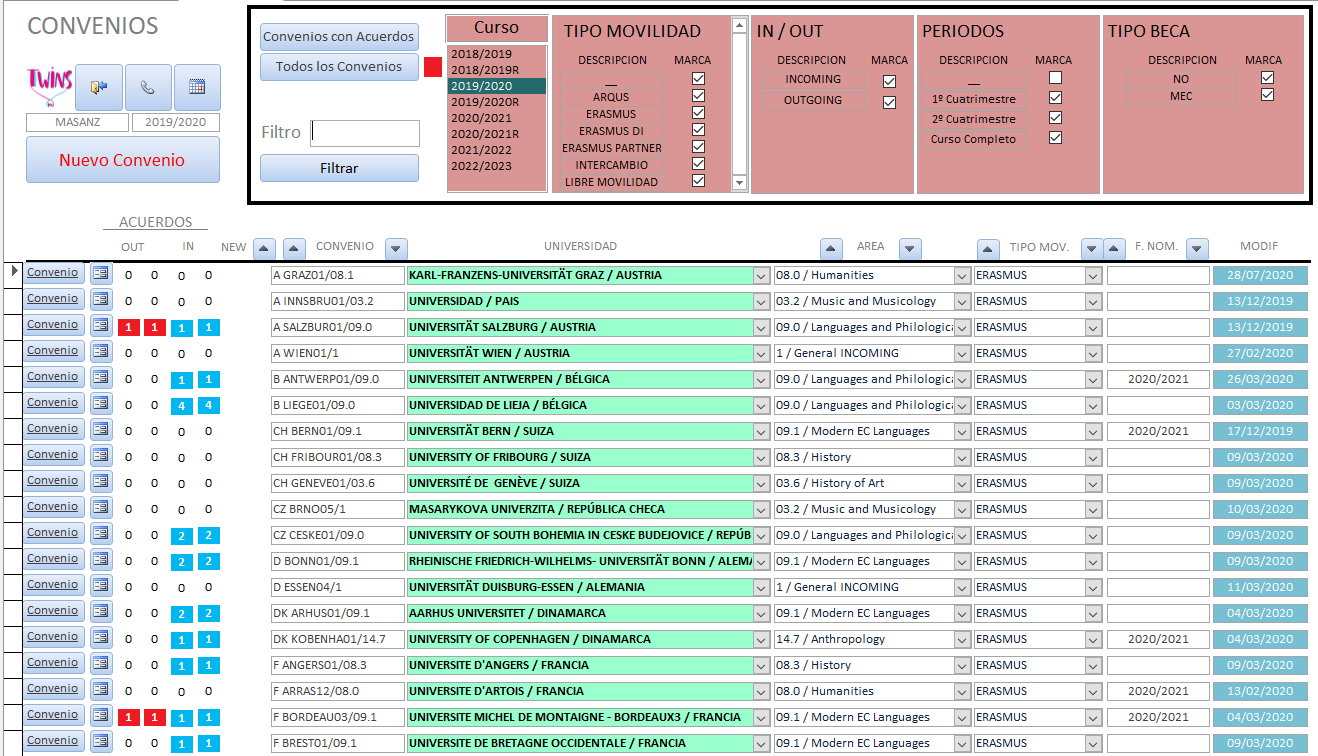
\includegraphics[width=\textwidth]{img/Capturas de TWINS/vistaConvenios.png}
	\caption[Convenios]{Vista de Convenios}
	\label{fig:vistaConvenios}
\end{figure}

\begin{table}[h]
	\begin{center}
		\begin{tabular}{ | c | c | } 
			\hline
			\multicolumn{2}{|c|}{\textbf{Administración}} \\
			\hline
			Estudiantes \footnotemark & 2055 \\ 
			\hline
			Tutores & 58 \\
			\hline
			Convenios  & 607 \\ 
			\hline
			Expedientes & 5049 \\ 
			\hline
			\multicolumn{2}{|c|}{\textbf{Base de datos}} \\
			\hline
			Tablas & 108 \\
			\hline
			Relaciones & 60 \\
			\hline
			Macros & 55 \\
			\hline
			Formularios & 152 \\
			\hline
			Consultas QBE & 343 \\
			\hline
		\end{tabular}
		\caption{Estadísticas de TWINS}
		\label{tab:estadisticasTWINS}
	\end{center}
\end{table}~
\footnotetext{Tanto \textit{incoming} como \textit{outgoing}}



\subsection{El modelo de datos}
\label{ModeloDatos}

El modelo relacional propuesto por Codd es el elegido para el diseño de esta base de datos. Las distintas tablas de la misma se conectan mediante relaciones que establecen restricciones para mantener la consistencia entre los datos.

Las tablas son una forma característica de almacenamiento de este modelo, en contraposición con otras disposiciones de la información usadas por otros sistemas y que, al fin y al cabo, se diseñan de otro modo porque se han de satisfacer unas necesidades distintas.

En este caso, podemos entender que la herramienta TWINS fue creada en Access y, por tanto, en un modelo de datos relacional dado el fácil acceso al usuario no experto en la materia, facilitando la operatividad con las bases de datos.

Es, sin duda, el modelo que más se utiliza aún hoy en día, el cual promete una determinada efectividad siempre y cuando el volumen de información a manejar no sea excesivamente elevado. En este caso, aunque la información que se requiere manipular en la oficina no es fácilmente manejable por personas, sí que aún podemos continuar utilizando este modelo para el desarrollo de la nueva herramienta twinX. Se entiende que no se tendrán más de unos 1000 estudiantes por curso académico (en una sola facultad) y que el número de convenios y tutores no será ni mucho menos parecido, considerando, eso sí, que la cantidad de \glspl{ExpedienteTWINS} será aproximadamente el doble que la de los estudiantes para los que se creen dichos registros.

Así pues, el modelo relacional parecer ser suficiente para las funcionalidades básicas y necesarias para trabajar en la ORI-FyL que twinX pretende implementar.

No obstante, no olvidemos la intención de extender la funcionalidad del actual TWINS para que los propios estudiantes puedan dejar atrás el constante envío de documentos entre sus tutores académicos por correo electrónico, de modo que puedan dar el salto a una plataforma que implemente una interfaz que les permita prescindir de estos documentos, como el acuerdo de estudios, y trabajar con la información directamente (aunque se posibiliten las conversiones a certificados que puedan ser impresos). En este contexto, se ha de tener en cuenta la forma de tratar los datos que se quiere realizar, que tendrá que adaptarse a este modelo de datos que va a ser usado también en twinX.

%Si todas las asignaturas de la universidad de origen se tienen en memoria y tan sólo se tienen que registrar las de la universidad de destino, tan sólo tendríamos que guardar códigos, órdenes y los nuevos nombres para esas asignaturas. Sin embargo, si esto se complicara y tuviéramos que almacenar documentos, quizás, para esa parte de la aplicación, sería conveniente estudiar la posibilidad de implementar una base de datos cuyo modelo de datos esté enfocado a la búsqueda de estos y, no menos importante, optimizado para dicho propósito, algo que sería impensable en una base de datos relacional. Un ejemplo de estas bases de datos es \textbf{Elasticsearch}, que permite hacer búsquedas complejas en texto, a través de datos estructurados y desestructurados. Esta podría ser una buena opción a utilizar una vez se alcance una determinada complejidad en el sistema de almacenamiento, pero en nuestro caso, solo lo comentamos como posibles trabajos futuros.

\subsection{Funciones implementadas}

\begin{itemize}
	\item \textbf{Funcionalidades básicas}\\
	Entre las funciones que hacen que TWINS cobre sentido, destacamos las siguientes:
	
	\begin{itemize}
		\item \textbf{Almacenamiento de información administrativa:} estudiantes, tutores, convenios, expedientes, etc.
		\item \textbf{Asociación de estudiantes con otras entidades:} estudiantes con su tutor, el convenio respecto del cual realizan su movilidad, sus expedientes, etc.
		\item \textbf{\gls{AM}}: para poder organizar a los estudiantes \textit{incoming}
		\item \textbf{Envío masivo de correos electrónicos:} posibilita funciones como las \glspl{Nominacion} automáticas o la comunicación a los participantes en los programas de movilidad de su tutor académico.
		\item \textbf{Generación de documentos automática:} disposición de los distintos datos en documentos que son entregables a estudiantes para mostrarles un sumario de su situación académica
		\item \textbf{Creación, edición y borrado de los datos dentro de la aplicación}
		\item \textbf{Anotación de futuras modificaciones a documentos ajenos a la oficina:} como son, por ejemplo, los convenios, que quedan registrados en la sede de la UGR y no pueden ser modificados hasta una fecha concreta, fuera del control de la ORI-FyL.
		\item \textbf{Recuperación de información de otros formularios externos a la aplicación:} para el registro de nuevos estudiantes (que es hasta ahora la mejor aproximación a la automatización de dicho proceso de la que se dispone) y, por ejemplo, para registrar datos de estudiantes afectados de alguna manera por la COVID-19.
	\end{itemize}

	\item \textbf{Funcionalidades específicas}\\
	Entre las que destacan la generación de informes con fines estadísticos para la oficina, información de asignaturas o menús para gestionar formularios creados por el personal para poder posteriormente transferir la información a la herramienta TWINS.
	
	También disponen de un sistema de alertas en relación con las tareas a realizar por el personal y con una especie de calendario donde se notifican los eventos temporales más próximos a atender.
\end{itemize}

\subsection{La interfaz de usuario}

Como hemos señalado en anteriores secciones, toda la aplicación yace sobre la herramienta de Microsoft\textregistered. Por ello, tanto los datos, como la presentación o vista y el control ejercido sobre los mismos no tiene separación alguna.

Al margen de esto y analizando las ventajas que el uso de Access\textregistered \ nos podría aportar, tenemos una manera de crear una interfaz de usuario de una manera más sencilla de lo normal. Tan sólo basta con arrastrar y redimensionar un botón con el ratón y una casilla para mostrar texto y con unas simples instrucciones tenemos una acción que, al pulsar el nuevo botón, en la casilla podría mostrarse, por ejemplo, cuántos registros almacena una determinada tabla (o varias de ellas) en la base de datos. Las consultas a la base de datos pueden almacenarse y reutilizarse según se quiera. A las interfaces se las conoce como \textbf{formularios} en Access\textregistered

También pueden programarse como si de una consulta se tratara, acciones que impliquen la modificación, borrado o creación de registros en la base de datos. A estas piezas de código funcionales se les da el nombre de \textit{macros}.

Una vez mencionadas las posibilidades funcionales, abordemos el uso de las mismas que han hecho para construir TWINS.

Lo primero que nos encontramos tras abrir la aplicación, es una pantalla de login con los distintos usuarios que pueden acceder al sistema (figura \ref{fig:login})

\begin{figure}
	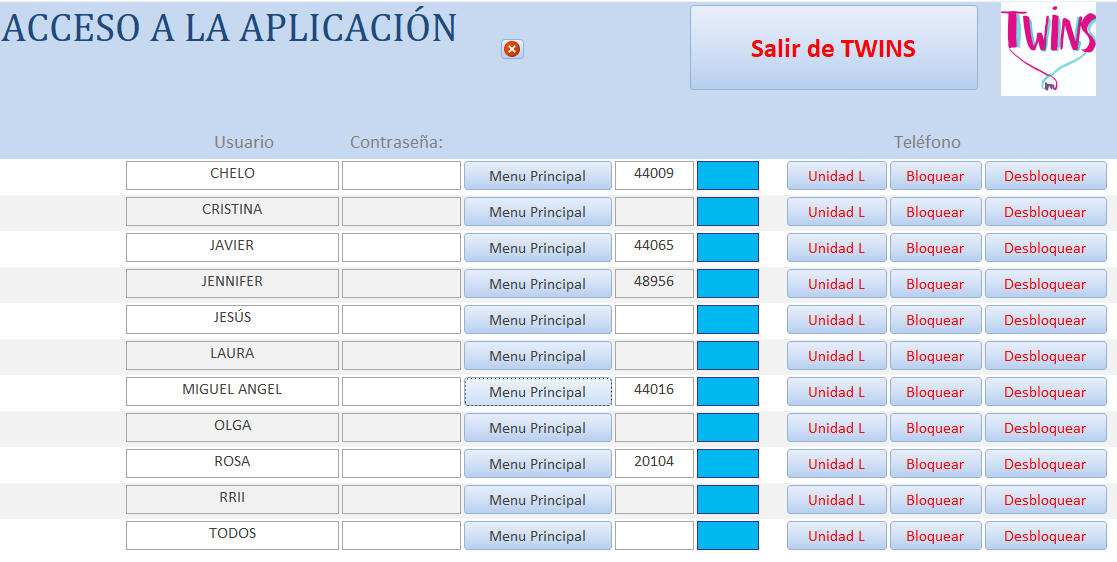
\includegraphics[width=\textwidth]{img/Capturas de TWINS/login.png}
	\caption[Login de TWINS]{Vista del login inicial de TWINS con todos los usuarios}
	\label{fig:login}
\end{figure}


Tras identificarnos, nos topamos, antes de llegar a la pantalla principal, con tres pantallas más:

\begin{itemize}
	\item El calendario (figura \ref{fig:calendario}) proporciona una vista genérica de todos los eventos que tienen lugar y que conciernen a la ORI-FyL o que tratan de asuntos relacionados con la misma. También se guardan plazos para realizar determinadas tareas. Los eventos del calendario\footnote{Nótese la especificación de «evento de calendario» o «\gls{EventoExpedienteTWINS}» en las definiciones correspondientes para establecer la diferenciación entre eventos que tienen que ver con la planificación en el calendario y los que componen los \glspl{ExpedienteTWINS}} son públicos a todos los usuarios de TWINS y en la creación de las entradas en él se permite establecer un(a) encargado/a de la tarea (figura \ref{fig:nuevatarea}), de modo que de un vistazo puedan verse los avisos pendientes que se tienen para un determinado evento.
	
	\begin{figure}
		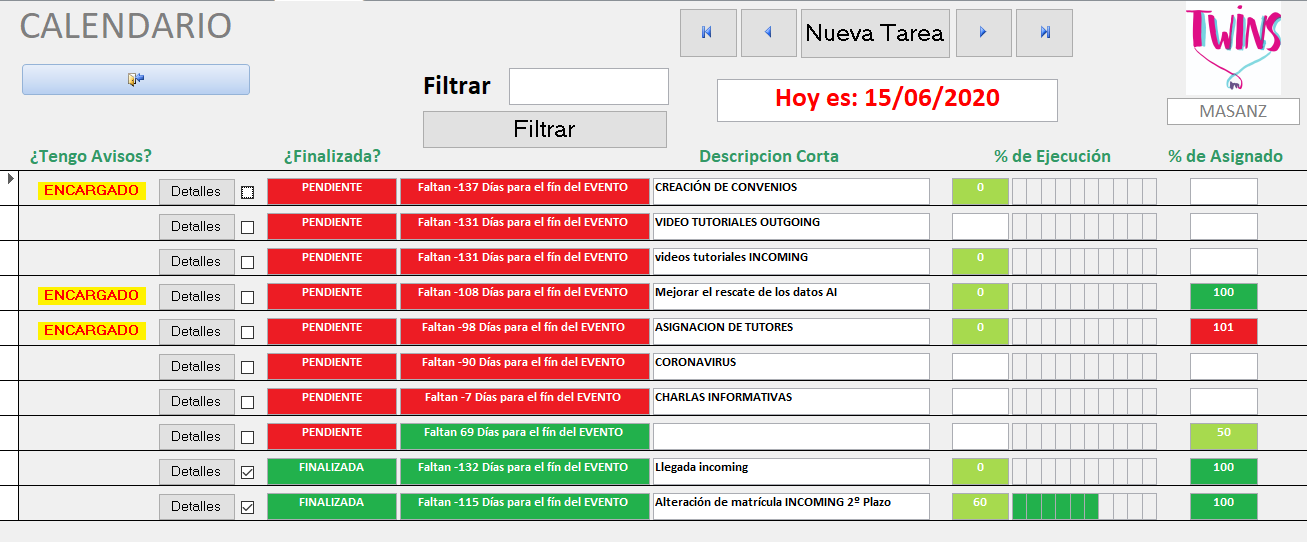
\includegraphics[width=\textwidth]{img/Capturas de TWINS/calendario.png}
		\caption[Calendario de TWINS]{Vista del calendario en TWINS con los eventos existentes y visibles por todos los usuarios}
		\label{fig:calendario}
	\end{figure}

\begin{figure}
	\centering
	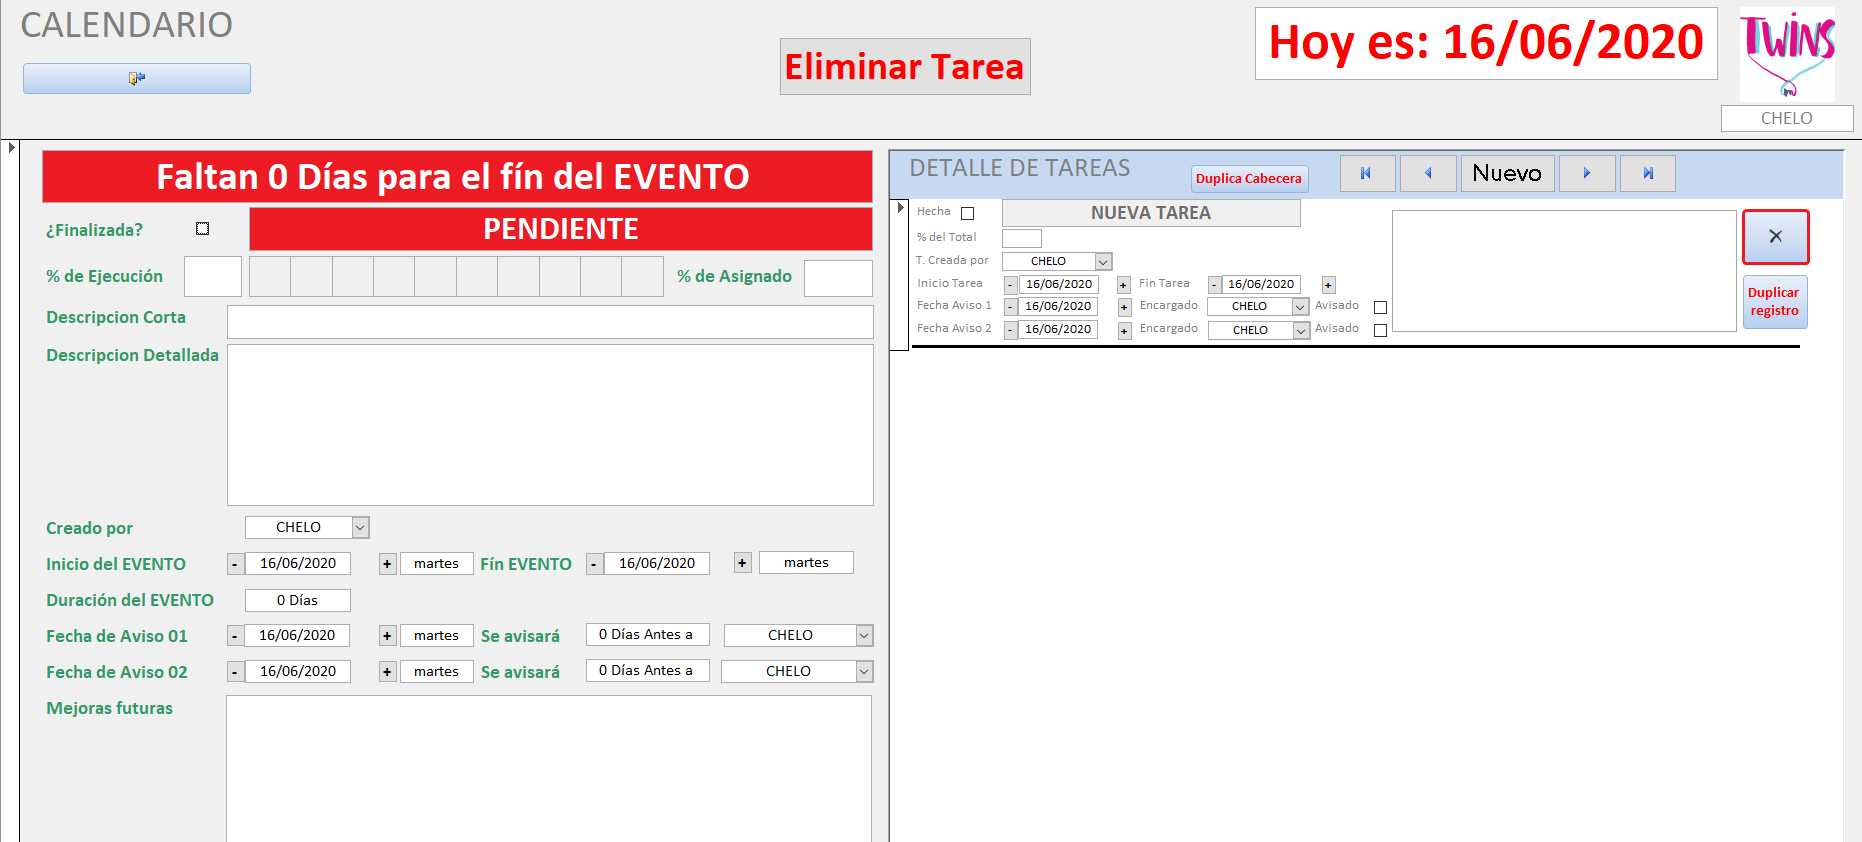
\includegraphics[width=\linewidth]{img/Capturas de TWINS/nuevaTarea}
	\caption[Creación de un nuevo evento en TWINS]{Creación de un nuevo evento en TWINS con la posibilidad de asignar tareas a otros usuarios}
	\label{fig:nuevatarea}
\end{figure}

	
	
	\item La pantalla de avisos (figura \ref{fig:avisos}) nos alerta de las acciones que tenemos que realizar con mayor urgencia, dado que han sido programadas para tenerlas listas para una fecha cercana y necesitan de la atención del usuario al que se notifica. Los avisos, al igual que un mensaje cualquiera, tienen emisor y receptor; es decir, hay alguien que los crea y los dirige a otra persona. Cuando se añade un evento al calendario, se especifican ambos actores, de modo que cuando está próxima la fecha de alguna tarea, se crea el aviso y notifica a aquel al cual le ha sido asignada. Normalmente, un usuario solo puede visualizar los avisos que le han sido dirigidos, salvo el administrador, quien puede ver todos los avisos de todos los usuarios aparte de los propios
	
	Por supuesto, también se pueden crear avisos fuera del contexto de los eventos de calendario, lo que también implica la existencia de emisor, receptor y fecha de caducidad. Al margen de la importancia que se le da a la notificación del número restante de días para que una tarea caduque, esta última forma de hacer uso de los avisos podría verse como imaginando al creador, en la oficina, dejando una nota adhesiva en la mesa de su compañero/a.
	
	 \begin{figure}
	 	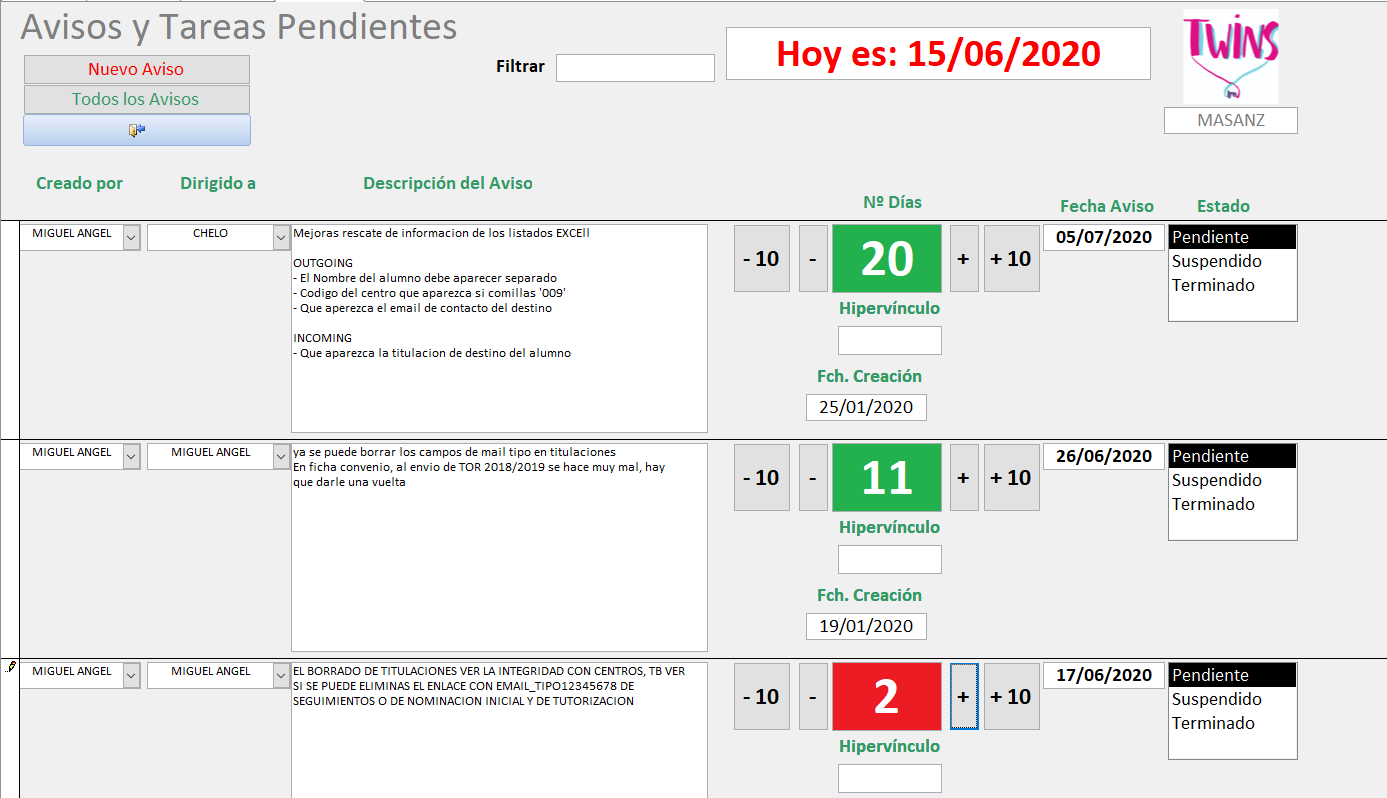
\includegraphics[width=\textwidth]{img/Capturas de TWINS/avisos.png}
	 	\caption[Avisos de TWINS]{Vista de los avisos en TWINS desde el usuario administrador}
	 	\label{fig:avisos}
	 \end{figure}
	 
	
	\item Dejando atrás los plazos y los eventos del calendario, otro elemento de gran importancia y con lo que trabajan día a día en la ORI-FyL (y no sólo en un cierto momento del cuatrimestre académico) son los \glspl{EventoExpedienteTWINS}. Pensemos que a diario surgen problemas, inconvenientes o simplemente hay que actualizar la situación de un estudiante. Por ello, la siguiente pantalla tras descartar las dos anteriores es la de eventos (de expediente) sin procesar (figura \ref{fig:eventosSinProcesar}).
	
	En ella, los usuarios de gestión pueden acceder a la información relacionada con el evento, como los demás eventos, los expedientes del alumno para el cual se está mostrando la información, o directamente las fichas del estudiante o el convenio en sí mismas.
	
	\begin{figure}
		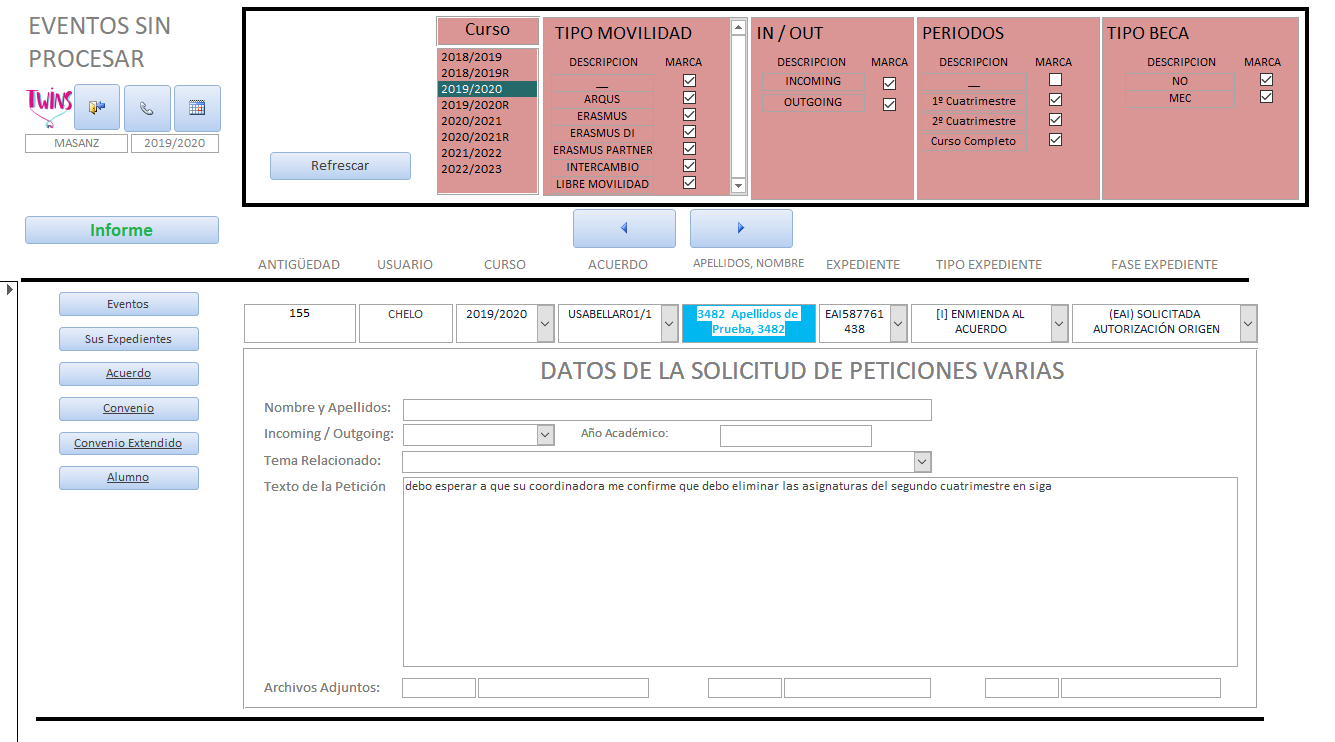
\includegraphics[width=\textwidth]{img/Capturas de TWINS/eventosSinProcesar.png}
		\caption[Eventos sin procesar de TWINS]{Menú de eventos sin procesar en TWINS, una pantalla donde los usuarios ven fácilmente el trabajo acumulado}
		\label{fig:eventosSinProcesar}
	\end{figure}
	
	
\end{itemize}

Finalmente, llegamos a la pantalla principal (figura \ref{fig:pantallaPrincipal}), de donde parten todos los menús (incluso los que acabamos de ver, que se muestran automáticamente identificarse correctamente en el sistema). En ella, no vemos ninguna información como la presentada en capturas anteriores (ni indicador de notificaciones, mensajes o alertas; nada). Lo que sí podemos apreciar es una selección en la cabecera de la vista principal con la que se filtrará el contenido que aparezca tras acceder a cualquier elemento del menú. Esto es, al solicitar determinada información cuando entremos a cierto menú, sólo se nos mostrarán aquellos datos que estén especificados en dicho cuadro de filtrado. Así, las consultas que se pueden hacer a la base de datos son mucho más cómodas y accesibles a todos los usuarios que no tienen por qué tener conocimiento de estos sistemas.

\begin{figure}
	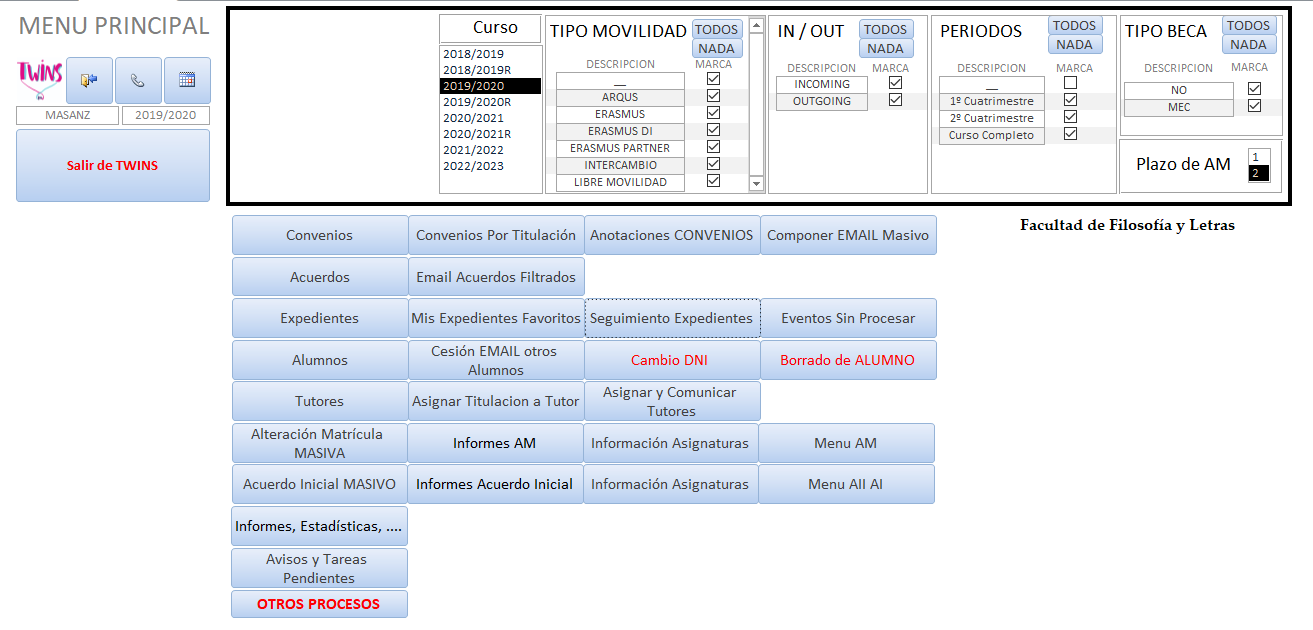
\includegraphics[width=\textwidth]{img/Capturas de TWINS/pantallaPrincipal.png}
	\caption[Menú principal de TWINS]{Pantalla principal de TWINS. Desde aquí podemos acceder a todos los menús anteriormente mostrados.}
	\label{fig:pantallaPrincipal}
\end{figure}

Si accedemos, por ejemplo, a la vista de convenios que ya hemos mostrado con anterioridad (figura \ref{fig:vistaConvenios}), el cuadro de filtrado se nos bloquea (ya hemos hecho una consulta y, para hacer otra, con otros parámetros, tendríamos que retroceder y volver a establecer nuestras preferencias de búsqueda). Se listan los convenios tal y como se han solicitado. El orden puede variarse a través de las flechas en las distintas columnas. Sin embargo y como es lógico, no se muestra toda la información de una tabla. Es más, realmente se están solicitando datos de distintas tablas (figura \ref{fig:tablasConsultaConvenios}). Este es un ejemplo de cómo la herramienta de creación de formularios de Access nos permite disponer la información de una tabla de forma más concisa que mostrando la tabla en crudo.

\begin{figure}
	\centering
	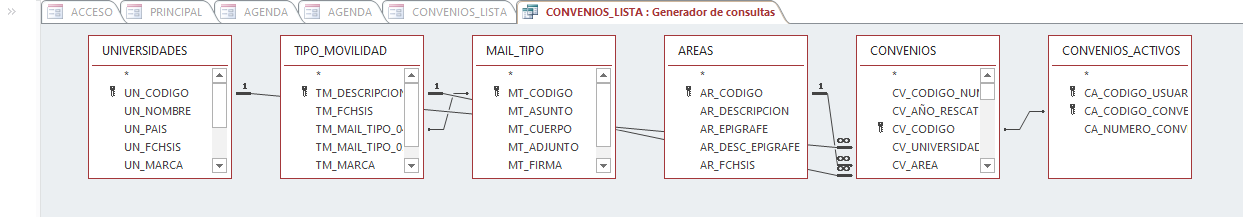
\includegraphics[width=\textwidth]{img/Capturas de TWINS/relacionTablasConsultaConveniosLista.png}
	\caption[Tablas implicadas en consultar convenios en TWINS]{Relación de tablas implicadas en la consulta realizada para listar los convenios en TWINS}
	\label{fig:tablasConsultaConvenios}
\end{figure}

Si nos fijamos en las distintas entradas de la lista en la figura \ref{fig:vistaConvenios} de nuevo, correspondiente cada una a un distinto convenio, vemos que se tienen elementos como un botón para acceder al formulario de la vista del mismo, los estudiantes \textit{outgoing} o \textit{incoming} que están de movilidad según ese convenio, y demás elementos que son de relevancia para la entrada en concreto.

A efectos de diseño de la interfaz, es apreciable que ciertos campos de cada entrada se presentan con un elemento de lista, también conocido como \textit{dropdown}. No son editables hasta que no se accede a la vista del convenio, en contra de lo que puede dar a entender. Si generalizamos al resto de la aplicación, existen numerosos elementos con una disposición extraña como la que mencionamos, de modo que resultan atípicos para el usuario inexperto, lo que podría llevar a confusiones y una pérdida de confianza en el usuario que interactúe con el sistema, a pesar de que no habrá gran cantidad de gente que comience a utilizar el sistema por primera vez de forma avanzada como es la labor del personal de secretaría, quienes sí lo harán. De todos modos, no podemos dar nada por hecho y la labor de un experto en informática es, en esencia, facilitar y mejorar.

Es por ello por lo que gran parte de este proyecto se enfocará al rediseño de la aplicación de TWINS basado en técnicas de usabilidad. Esto será posible gracias a la aplicación de metodologías actuales y la realización de pruebas reales con usuarios que interaccionarán con el sistema.

Para finalizar, vamos a comentar aspectos genéricos sobre las distintas vistas de la interfaz de TWINS. Es un elemento apreciable el uso de colores vivos y que reclaman la atención del usuario. Éstos suelen ser utilizados mayormente en áreas donde se debe prestar mucha atención y se debe proceder con cuidado a la hora de hacer cambios, pues podría desencadenar a un estado de inconsistencia en el sistema difícil de revertir. Ejemplo de esto es el menú de cambio de DNI (figura \ref{fig:cambioDNI}), donde la cabecera es amarilla. La propia aplicación te impide editar el DNI si para el estudiante seleccionado se tienen registros de información. No obstante, no cabe duda de que se trata de un cambio importante, y por eso también, para acceder a dicho menú, hay que hacer doble click en el botón del menú principal (figura \ref{fig:pantallaPrincipal}), ya que sus letras tienen un color rojo, como pasa con cualquier botón que contiene la aplicación y se resalta de esta manera.

También, como elemento en común cada vez que aparece el nombre de los estudiantes, se marca en rojo si es \textit{outgoing} o en azul si, por el contrario, es \textit{incoming}. Ejemplos de esto podemos encontrarlos en las figuras \ref{fig:alumnos} y \ref{fig:cesionDeDatos}. En la primera, podemos también apreciar cómo se presenta un color verde en la columna de casillas más a la izquierda cuando el número de acuerdos de estudios activo para los estudiantes es de 0, lo que significa que «no hay peligro» al editar su información. Si por el contrario tuvieran más de uno, la aplicación mostraría la cifra en amarillo, indicando el alto riesgo de modificar sus datos en caso de hacerlo de forma descuidada. Nótese que no se muestran datos con carácter sensible debido a cuestiones de protección de datos.

Comentemos, en último lugar, que la disposición de estos colores e indicadores no es en vano, no ya a partir de las aclaraciones anteriores, sino también haciendo alusión a la figura \ref{fig:infoAsignaturas}, donde no se tienen datos importantes que modificar, tan solo se trata de una mera consulta --sin derecho a modificación-- a las asignaturas registradas para los estudiantes en la base de datos, no habiendo riesgo de comprometer la consistencia de la información. Es por ello por lo que la paleta de colores, aunque de discutible empleo en toda la aplicación, es muy reducida en esta vista concretamente, pues tan solo se resalta en azul la cabecera, y el resto queda en blanco y negro.


\begin{figure}
	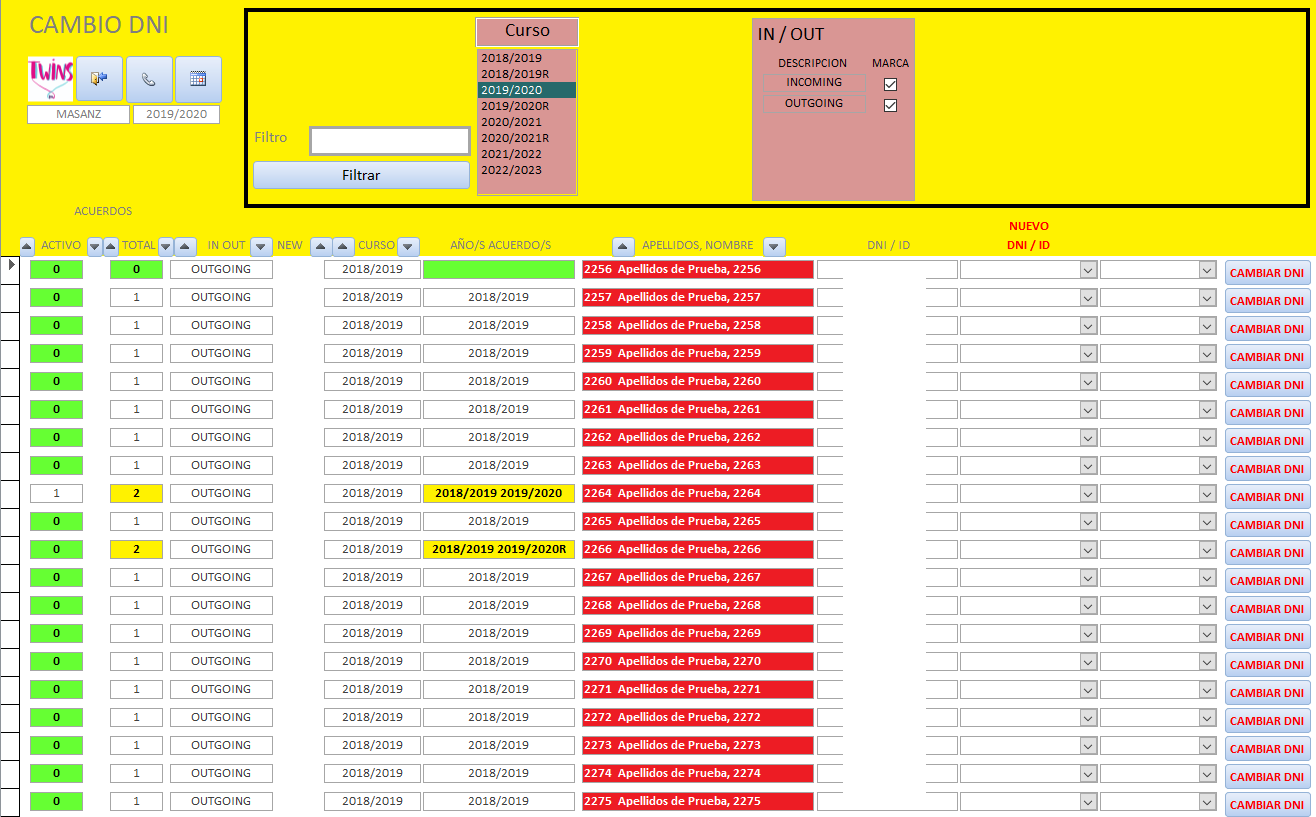
\includegraphics[width=\textwidth]{img/Capturas de TWINS/cambioDNI.png}
	\caption[Menú de cambio de DNI]{También existe en TWINS un menú específico para el cambio de DNI}
	\label{fig:cambioDNI}
\end{figure}

\begin{figure}
	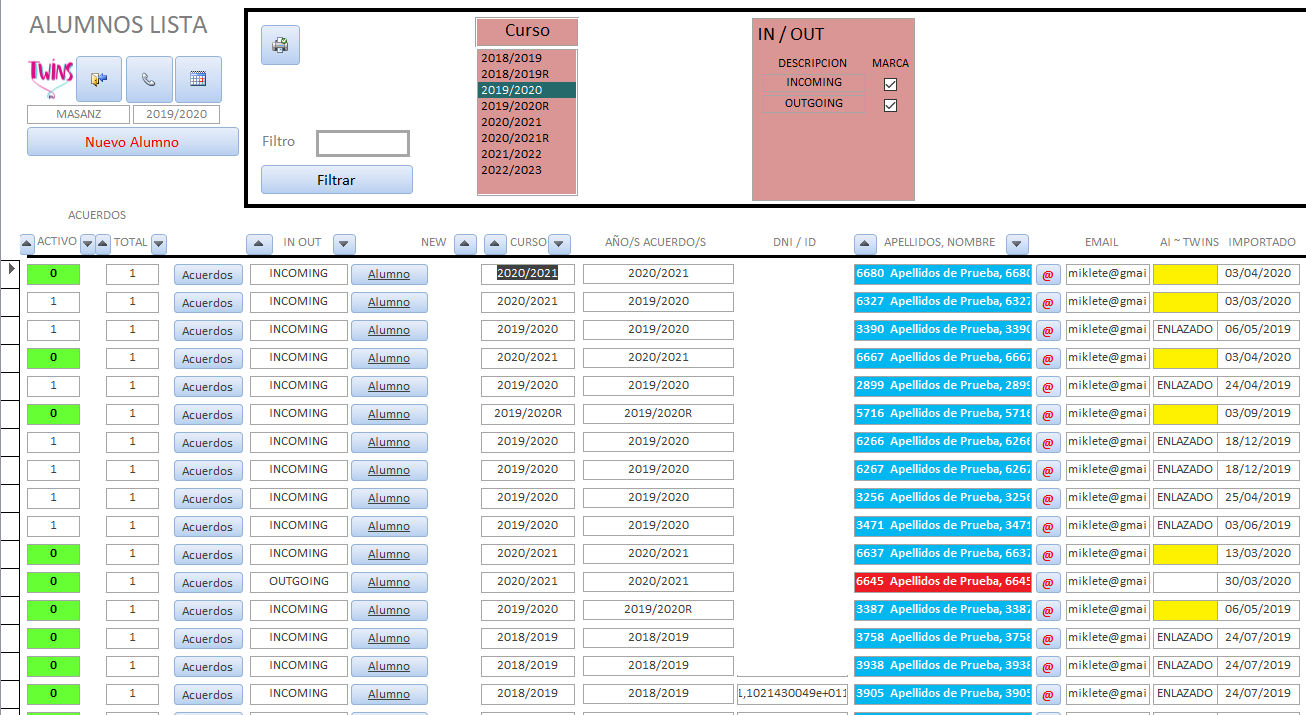
\includegraphics[width=\textwidth]{img/Capturas de TWINS/alumnos.png}
	\caption{Vista de alumnos en TWINS}
	\label{fig:alumnos}
\end{figure}

\begin{figure}
	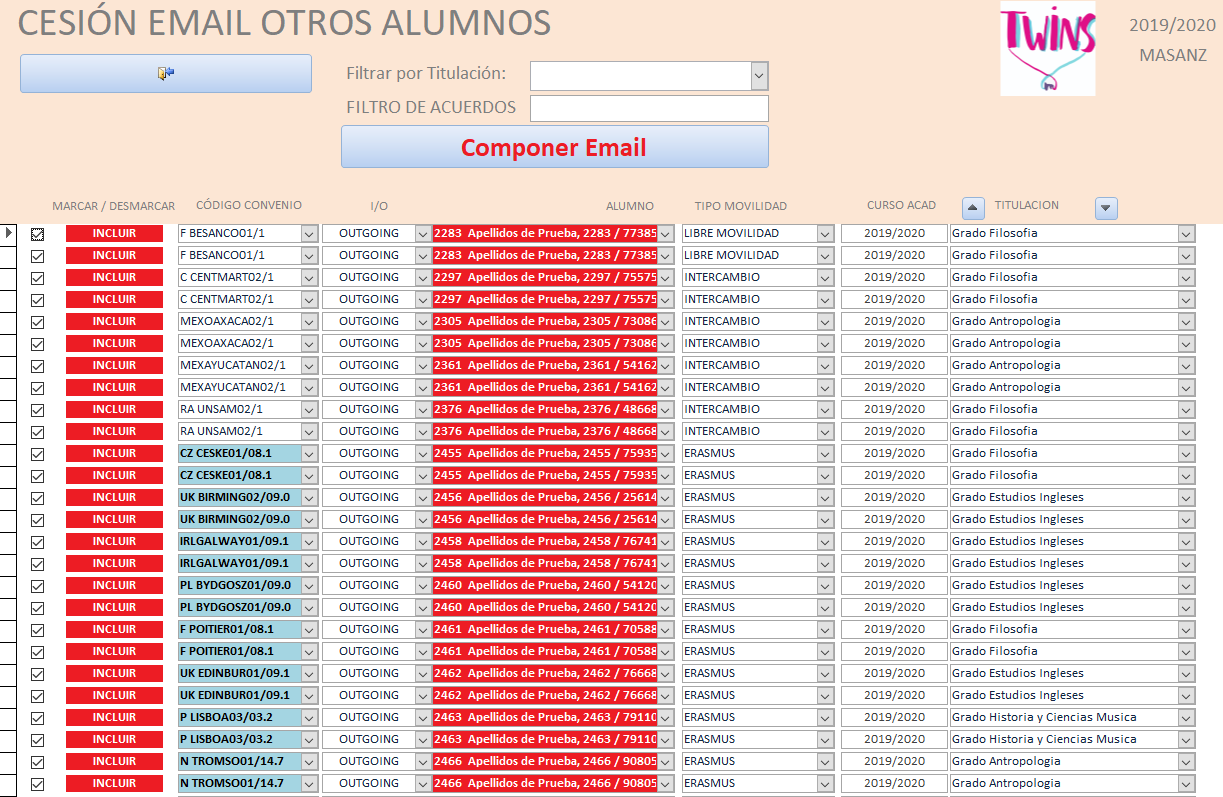
\includegraphics[width=\textwidth]{img/Capturas de TWINS/cesionDeDatos.png}
	\caption[Consentimiento de datos en TWINS]{Menú de gestión del consentimiento de cesión de datos de los estudiantes salientes en TWINS}
	\label{fig:cesionDeDatos}
\end{figure}

\begin{figure}
	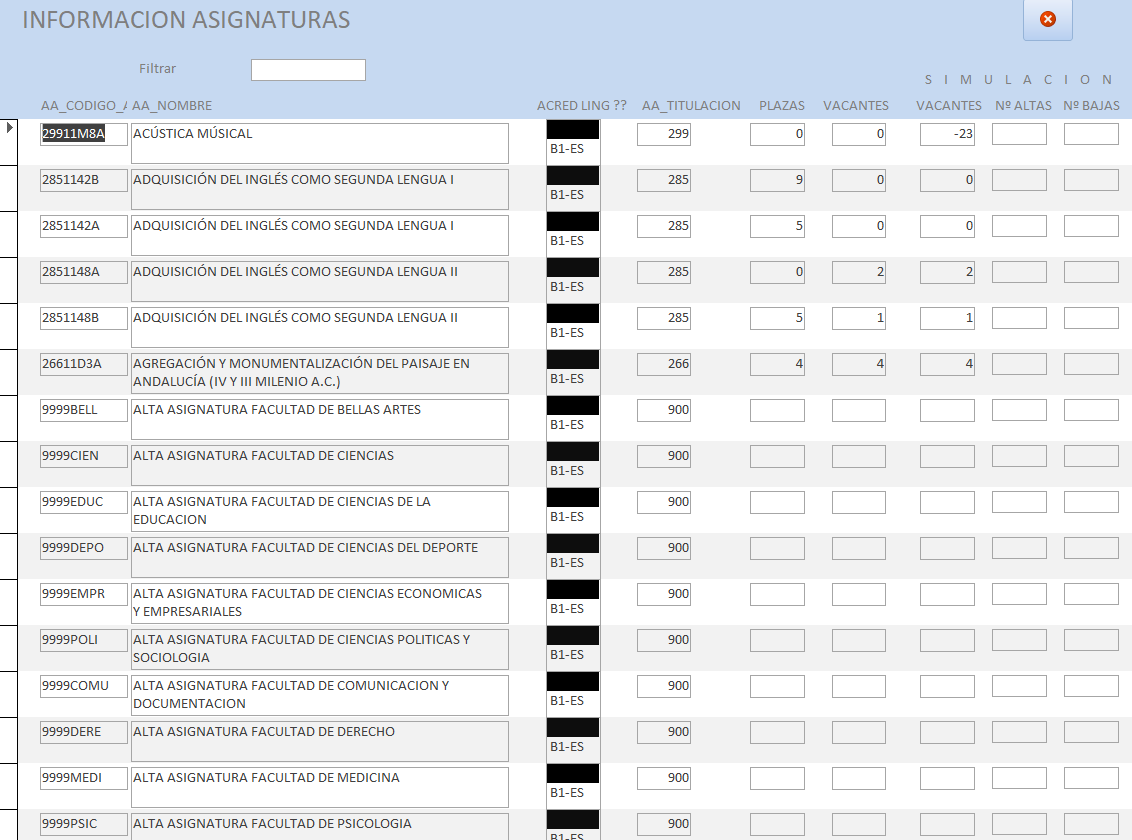
\includegraphics[width=\textwidth]{img/Capturas de TWINS/infoAsignaturas.png}
	\caption[Vista de información de asignaturas en TWINS]{Menú de información de las asignaturas en TWINS (en la universidad local, de destino, de cara a los estudiantes entrantes)}
	\label{fig:infoAsignaturas}
\end{figure}



\section{Estudio de necesidades de la ORI-FyL}

En general, la Oficina de Relaciones Internacionales de la facultad dispone de una herramienta que, dado que ha sido creada por un integrante de la secretaría de la facultad con una estrecha relación laboral con los miembros de la oficina, ha sabido cumplir los requisitos  operacionales del servicio. Muchas funcionalidades de la misma son muy concretas a las necesidades de la ORI-FyL (informes imprimibles con documentación específica, estadísticas, pegatinas para fundas de plástico, etc.)

No obstante, debido a las limitaciones de la metodología escogida para posibilitar estas gestiones, se ha llegado a un punto en que es muy complicado realizar modificaciones y extensiones a la misma. Por ejemplo, la ORI-FyL destaca la necesidad de un portal directamente conectado a la aplicación principal que posibilite la realización de gestiones por parte de los estudiantes. De este modo, tanto el estudiante como el personal de secretaría ahorrarían tiempo y su interacción no sería íntegramente en el correo electrónico. Esto es también extensible al papel de los tutores académicos.

Actualmente se ha hecho uso de herramientas auxiliares como los Formularios de Google\textregistered \ que permiten volcar datos al formato de hoja de cálculo, con lo que permite a TWINS reconocer la información y que pueda, a través de macros, crear nuevos registros en la base de datos para almacenarlos. Sin embargo, se precisa de la interacción humana para dicha tarea, al igual para muchas otras que se puedan querer automatizar o adaptar, como por ejemplo:

\begin{itemize}
	\item \textbf{Adaptar la mensajería} e implementarla dentro de la aplicación para llevar un mejor control de los casos de los estudiantes.
	\item \textbf{Automatización del seguimiento de las nominaciones} teniendo un portal externo donde otras universidades puedan nominar a sus estudiantes en la UGR.
	\item \textbf{Portal con vista para el estudiante entrante}, posibilitando que haga su propio registro en la plataforma y pueda ver su información en ella.
\end{itemize}

Al margen de las nuevas características a incluir, no podemos dejar de lado la necesidad de reconstruir un sistema desde cero, para que sea consistente, estable, con alta disponibilidad y fiabilidad y que pueda adaptarse a las necesidades tanto del personal de la oficina como a las del estudiantado. Es por tanto por lo que debemos descartar seguir utilizando la herramienta de Access\textregistered \ dadas sus limitaciones, expuestas en la sección \ref{ModeloDatos}.

% 3. twinX

\chapter{twinX}

Una vez hemos analizado el material ya existente y desde el que partiremos para la construcción de twinX, vamos a ponernos manos a la obra con su desarrollo. Si bien es cierto que no se parte desde cero en cuanto a requisitos, sí que se va a reconstruir la herramienta desde cero, para poder aportar un gran significado a todos los módulos que vayan a formar parte de twinX y así podamos cohesionarlos de una mejor manera.

\section{Desarrollo de twinX}

Vamos a comenzar estableciendo las ideas principales del proyecto, reafirmando el propósito y viéndolo desde otras perspectivas que, aunque parecen obvias, no siempre se tienen en cuenta. Ello nos permitirá asentar las bases del producto software final y dotarlo de calidad.

\subsection{Diseño centrado en el usuario}

Esta disciplina, conocida también como \textit{User-Centered Design} o UCD, destaca por basar las fases del proceso de diseño estableciendo un enfoque constante en aprender del sujeto que utilizará el producto final. Es decir, para la consecución de los objetivos, es necesario tener una retroalimentación constante por parte del usuario final, que será quien vaya orientando nuestros avances según sea su interacción con lo que vayamos desarrollando.

El proceso dispone de unas fases a seguir, como son:
\begin{itemize}
	\item \textbf{Especificación del contexto de uso:} quiénes usarán el producto, para qué y bajo qué condiciones lo harán.
	\item \textbf{Especificación de requisitos:} identificar los objetivos que tienen que cumplirse para dejar a los usuarios satisfechos.
	\item \textbf{Crear soluciones de diseño:} en distintas etapas, desde un concepto poco definido hasta un diseño completo.
	\item \textbf{Evaluación de los diseños:} a través de las pruebas con los usuarios, de forma ideal.
\end{itemize}

\subsubsection{Pautas de Accesibilidad}

El no atender a causas de accesibilidad sería no aplicar correctamente, de alguna forma, el tipo de diseño escogido para el desarrollo del producto. Cuando se hacen pruebas, el objetivo no es otro que adaptar el producto para que pueda ser bien utilizado por el mayor número de usuarios posible y de la forma satisfactoria para ellos. Es por ello por lo que tenemos que abrir el abanico y contemplar que pueden ser numerosos los usuarios que necesiten adaptaciones para interaccionar correctamente con el contenido web.

Para ello, se propone la utilización de los recursos especificados en \textit{Web Content Accessibility Guidelines} (WCAG) \cite{wcag}. Con ello, podemos hacer que la experiencia en el sitio web pueda ser mínimamente satisfactoria para todo usuario que necesite hacer uso de la misma. En efecto, se deberán emplear una serie de técnicas, especificadas en su web, para que twinX sea adaptable. Entre ellas, destacamos la viabilidad de la interacción con el teclado, un texto descriptivo para las posibles imágenes que se puedan incluir, regular el contraste, etc. Con este proyecto, la intención es alcanzar el nivel AA (segundo más exigente), para que la gran mayoría de personas con necesidades especiales puedan usar la plataforma sin problema alguno.

\subsubsection{Encuesta SUS}

La encuesta SUS o \textit{System Usability Scale} es una de las encuestas que se pueden utilizar para evaluar la usabilidad de una cantidad de productos o servicios.

Sus únicos 10 enunciados es una de las cosas que más atractiva la hacen, puesto que hace que los usuarios la rellenen de manera rápida y fácil. También destaca por ser de denominación común y tener un bajo coste, además de poder corregirse inmediatamente después de terminar la encuesta. Es más, es una encuesta que puede aplicarse a casi cualquier tipo de interfaz de usuario, por lo que es muy versátil. Finalmente, cabe destacar la facilidad de entender los resultados, puesto que vienen dados en forma de una puntuación en el rango de 0 a 100.

Sobre los enunciado de la encuesta, tienen una escala de 1 a 5 cada uno, siendo 1 el indicador de mayor desacuerdo y el 5 el de mayor acuerdo. También se suele aportar unas pequeñas instrucciones a los candidatos a tomar la encuesta, indicando la necesidad de contestar todas las preguntas y de no pensarse mucho la respuesta a las mismas.

Para probar la eficacia de esta herramienta como elemento conductor en la creación de una interfaz de usuario a la hora de hacer pruebas y recibir \textit{feedback}, se hizo un experimento con una escala con adjetivos y no con números. Los resultados del análisis (\cite{sus}) vieron una mayor desviación de los resultados a la hora de expresar un mayor desacuerdo (adjetivos como «horrible» o «peor que lo imaginable» con números más próximos al 1). No obstante, en general, y gracias a análisis como el mencionado, se tiene evidencia que asegura que este tipo de encuestas es una buena herramienta a tener en cuenta a la hora de recibir información acerca de cuán bueno es nuestro diseño para los usuarios.

Por todo ello, esta será una de las herramientas que utilizaremos en las pruebas para constatar que los objetivos del proyecto se cumplen y cuáles pueden ser las conclusiones.

\subsection{\textit{Design Thinking}, DT}

El «Pensamiento de Diseño» o \textit{Design thinking} es una técnica de desarrollo que se centra en el usuario, pudiendo detectar y reaccionar ante cambios repentinos en el entorno de los usuarios y sus comportamientos. El objetivo está, mayormente, en abordar problemas con una pobre definición o que no se conocen a fondo para situar al usuario en el centro de todo y poder así enfocar el problema desde otras perspectivas, de manera que se pueda poner la atención en aquello que resulte de mayor importancia para los usuarios.

\subsubsection{Las fases del DT}

El proceso tiene unas fases no necesariamente secuenciales, de modo que puedan adaptarse lo mejor posible al proyecto, teniendo incluso la posibilidad de ejecutarse al mismo tiempo.

\begin{itemize}
	\item \textbf{Empatizar}, tratar de adoptar un conocimiento lo más empático posible del problema que se pretende resolver. Este es un elemento esencial, pues posibilita a los desarrolladores a descartar sus propias primeras conclusiones --erróneas a menudo-- y a entrar en materia con la realidad del cliente y sus necesidades.
	
	\item \textbf{Definir} las necesidades de los usuarios y sus problemas. Es la fase donde se reúnen y ordenan los elementos obtenidos como resultado de la fase anterior. A partir de entonces, se sintetizan para definir los problemas esenciales que se identifican, los cuales dan pie a la creación de \textit{personas}; esto es, la construcción de perfiles humanos en los cuales centrar el desarrollo.
	
	\item \textbf{Idear} y hacer frente a lo que se da por hecho, creando formas alternativas de ver y tratar el problema con soluciones innovadoras, a partir de lo estudiado en las dos fases anteriores.
	
	\item \textbf{Prototipado} de las soluciones pensadas, una fase experimental cuyo objetivo es el de encontrar la mejor solución para cada uno de los problemas encontrados. Los desarrolladores han de producir una versión de bajo coste del producto para investigar cuál es el resultado de haber llevado las ideas a la práctica.
	
	\item \textbf{Pruebas} con lo obtenido, para analizar si realmente se ha llegado a un buen resultado o, si por el contrario, se ha de retroceder a otra fase para redefinir uno o más problemas.
	
\end{itemize}

Como hemos indicado, las fases no siempre siguen el mismo orden. Hay veces que se toman decisiones como la de saltar de la primera fase de empatía a la penúltima de prototipado, probablemente para aclarar las ideas y poder hacer una mejor definición, a través de la muestra de material al cliente que pueda animarlo a dar una mayor retroalimentación. Del mismo modo, si el prototipado no ha ido bien, se puede volver a la tercera y anterior fase, la de construcción de ideas. Incluso podría darse el caso que haciendo pruebas, los desarrolladores nos demos cuenta de que no se ha llevado a cabo una buena ejecución del proceso y sea preciso volver a la segunda etapa de definición de los problemas. Siempre es mejor ir hacia atrás en lugar de comenzar la casa por el tejado, así que toda maniobra que sea apropiada para una mejor construcción del producto y que lo dote de calidad siempre es bienvenida.


\subsubsection{Herramientas del DT}
\label{herramientasDT}

Hay una serie de actividades o técnicas que nos pueden resultar útiles para llevar a cabo el trabajo de desarrollo con eficacia y que suelen tener éxito. Destacamos las siguientes:

\begin{itemize}
	\item \textbf{Creación de personas:} perfiles ficticios de los distintos usuarios que utilizarán el producto software. Creadas en la fase de definición, no solo se especifica el propósito específico de interacción con el producto a mejorar o la necesidad por que exista el software que se quiere desarrollar. Describimos el contexto del personaje, sus inquietudes y, en definitiva, lo que hay detrás de esa persona en más ámbitos que puedan ayudar a comprender por qué es necesario que se tengan en cuenta ciertas cosas a la hora del desarrollo.
	
	\item \textbf{\textit{Brainstorming}:} también conocida como nube de ideas que radican alrededor de un concepto central. Se trata de escribir conceptos que vengan a la cabeza de los intervinientes en la creación del esquema, sin importar los análisis o el futuro que puedan tener en el proceso. Cualquier cosa que tenga que ver con lo que se está tratando es válida, pues lo que aparentemente resulta absurdo podría en muchos casos resolver parcialmente el problema o ayudar a enfocarlo. Así, cuantas más propuestas, mejor se lleva a cabo este proceso, que tiene lugar en la fase de ideación.
	
	\item \textbf{Prototipado en papel:} la creación de prototipos (en la cuarta fase de prototipado) con un material del que todos disponemos es extremadamente sencilla a la par que útil. Cuando las cosas se plasman en un folio, podemos apreciar matices que no nos venían a la cabeza cuando la idea era tan solo un concepto. Si bien es cierto que depende de las dotes artísticas de la persona que dibuja el prototipo, el hacerlo con papel y lápiz ayuda a volcar la concentración de una manera diferente a como se hace cuando se programa o se diseña con herramientas informáticas.
	
	\item \textbf{Mapas de experiencia de usuario:} también conocidos como \textit{Customer Journey Maps}, sirven para representar la experiencia de un usuario a lo largo del tiempo. En ellos plasmamos la forma en que un diseño cubre o no las necesidades de un usuario utilizando un producto o servicio. Es justo por eso por lo que estos mapas han de ser lo más descriptivos posibles, representando con gran detalle las acciones y subtareas que tiene que desempeñar un usuario al usar el sistema.
	
\end{itemize}

\subsection{Aplicación de las metodologías}

En relación con las fases del DT, podemos diferenciar a través de las cuales ya hemos ido pasando. El comienzo del proyecto vino acompañado de una serie de reuniones que se incluyen en los anexos. En este contexto, la fase de \textbf{empatización} se correspondería con las dos primeras reuniones, donde se establecieron un primer contacto y las bases del proyecto, atendiendo al testimonio de los usuarios reales de TWINS, lo que actualmente se está usando para resolver los problemas a los que se tienen que enfrentar en la ORI-FyL. Es más, en la segunda reunión (~\ref{reunion2}) se habló de algunas características ideales y que está costando implementar en el actual escenario, lo que podríamos englobar dentro de la \textbf{ideación}. Por último, ya en la tercera reunión, se tiene la \textbf{definición} de todos los conceptos necesarios para comprender el funcionamiento de TWINS y de la oficina en general. No obstante, a lo largo de esta sección, vamos a continuar esta fase con la definición de más elementos necesarios para llevar a cabo el desarrollo de twinX.

Con esas tres fases cubiertas, se puede dar comienzo a las otras dos: la de \textbf{prototipado} y \textbf{pruebas}, que serán desarrolladas de forma más extensa en las secciones ~\ref{bocetos} y ~\ref{pruebas}. %PENDIENTE: comprobar referencias, ya que han sido puestas antes de tiempo y añadir posibles futuras reuniones y sesiones de pruebas.

\section{Personas ficticias}

Tal y como hemos comentado en la sección \ref{herramientasDT}, una de las herramientas que nos permiten definir el alcance y las necesidades de la aplicación es la creación de perfiles de personas ficticias, candidatos a utilizar twinX en un futuro. De esta forma, tanto por la parte del desarrollo como por la del interesado en el producto final, pueden no solo hacerse una mejor idea de los objetivos del mismo, sino también justificar su creación.

Vamos a tratar de crear tres personalidades lo más variopintas posibles en aras de enfocarnos más aún en el usuario y dotar de mayor calidad el resultado final, de modo que podamos abarcar por completo el entorno de influencia del problema. (Herramienta: \cite{uxpressia})

\begin{figure}
	\centering
	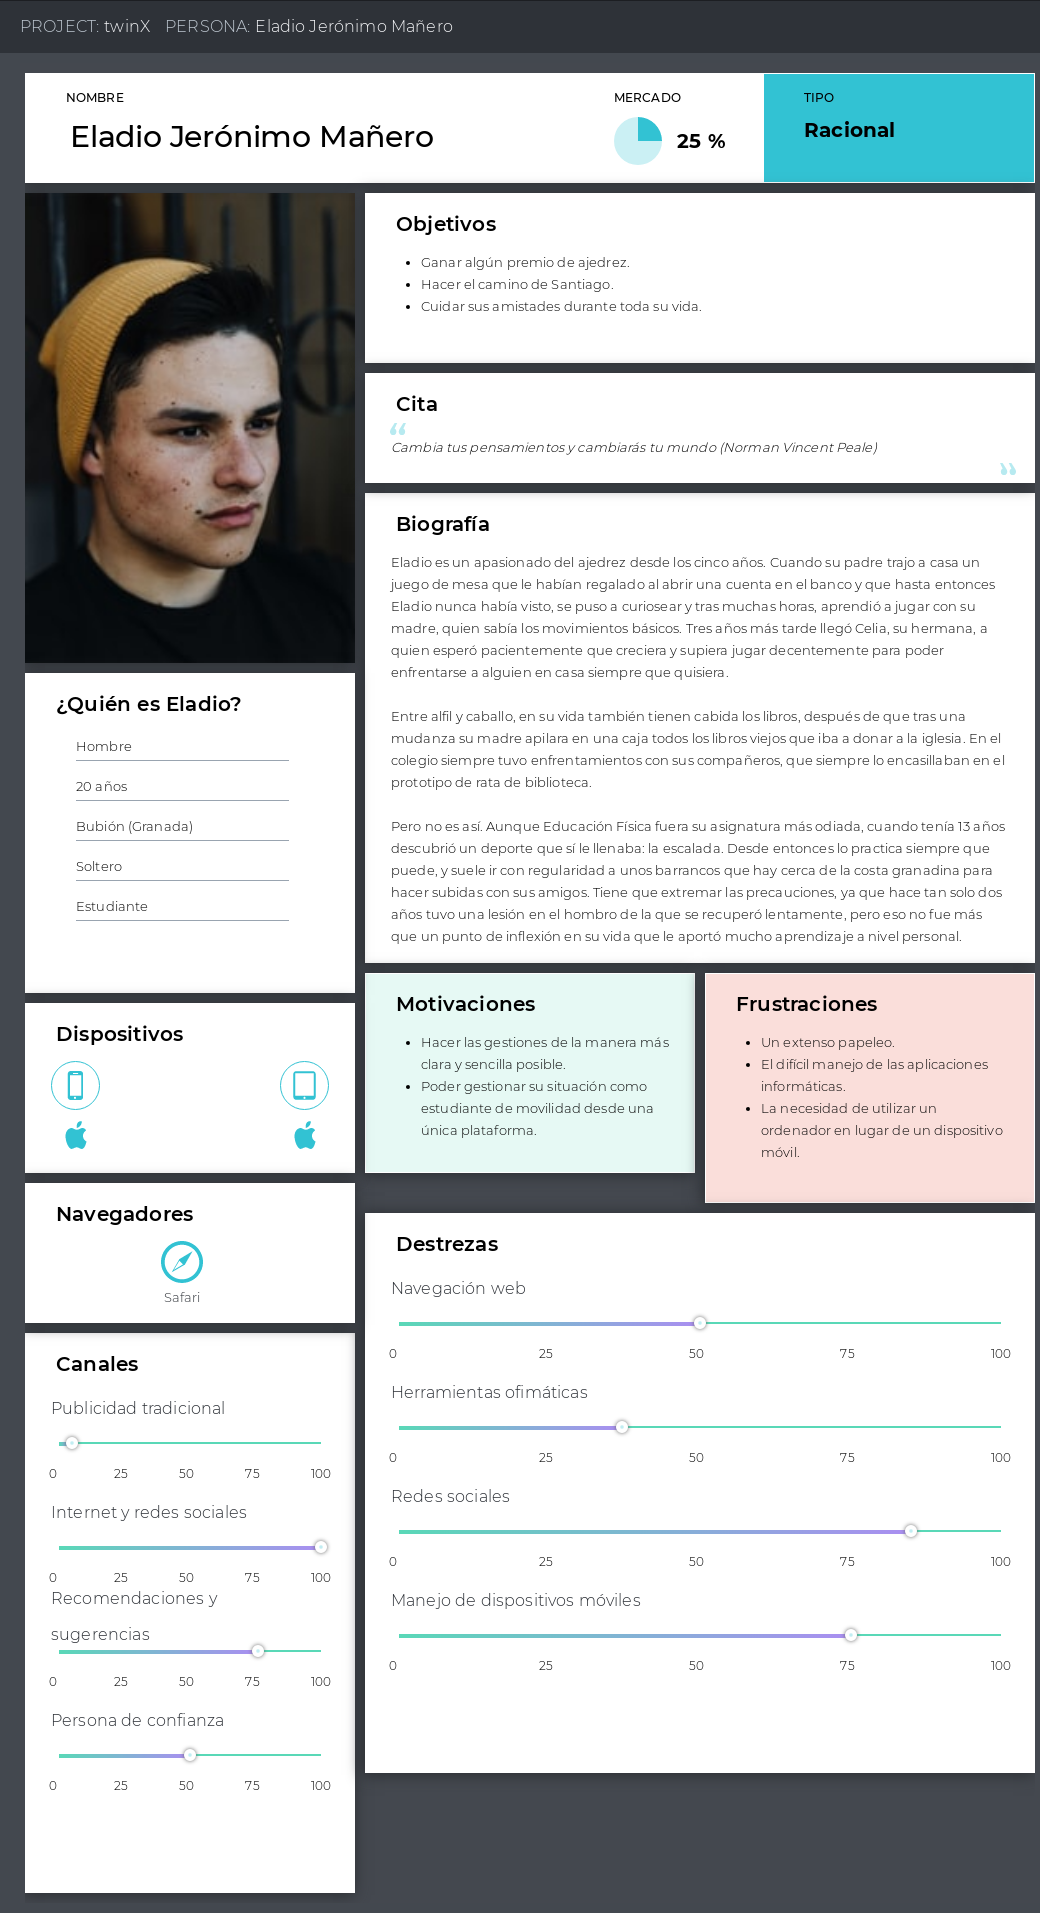
\includegraphics[width=\textwidth, height=\textheight, keepaspectratio]{img/Personas/Eladio}
	\caption[Persona \#1]{Persona \#1: Eladio}
	\label{fig:persona1}
\end{figure}
\begin{figure}
	\centering
	\includegraphics[width=\textwidth, height=\textheight, keepaspectratio]{img/Personas/MGracia}
	\caption[Persona \#2]{Persona \#2: María Gracia}
	\label{fig:persona2}
\end{figure}
\begin{figure}
	\centering
	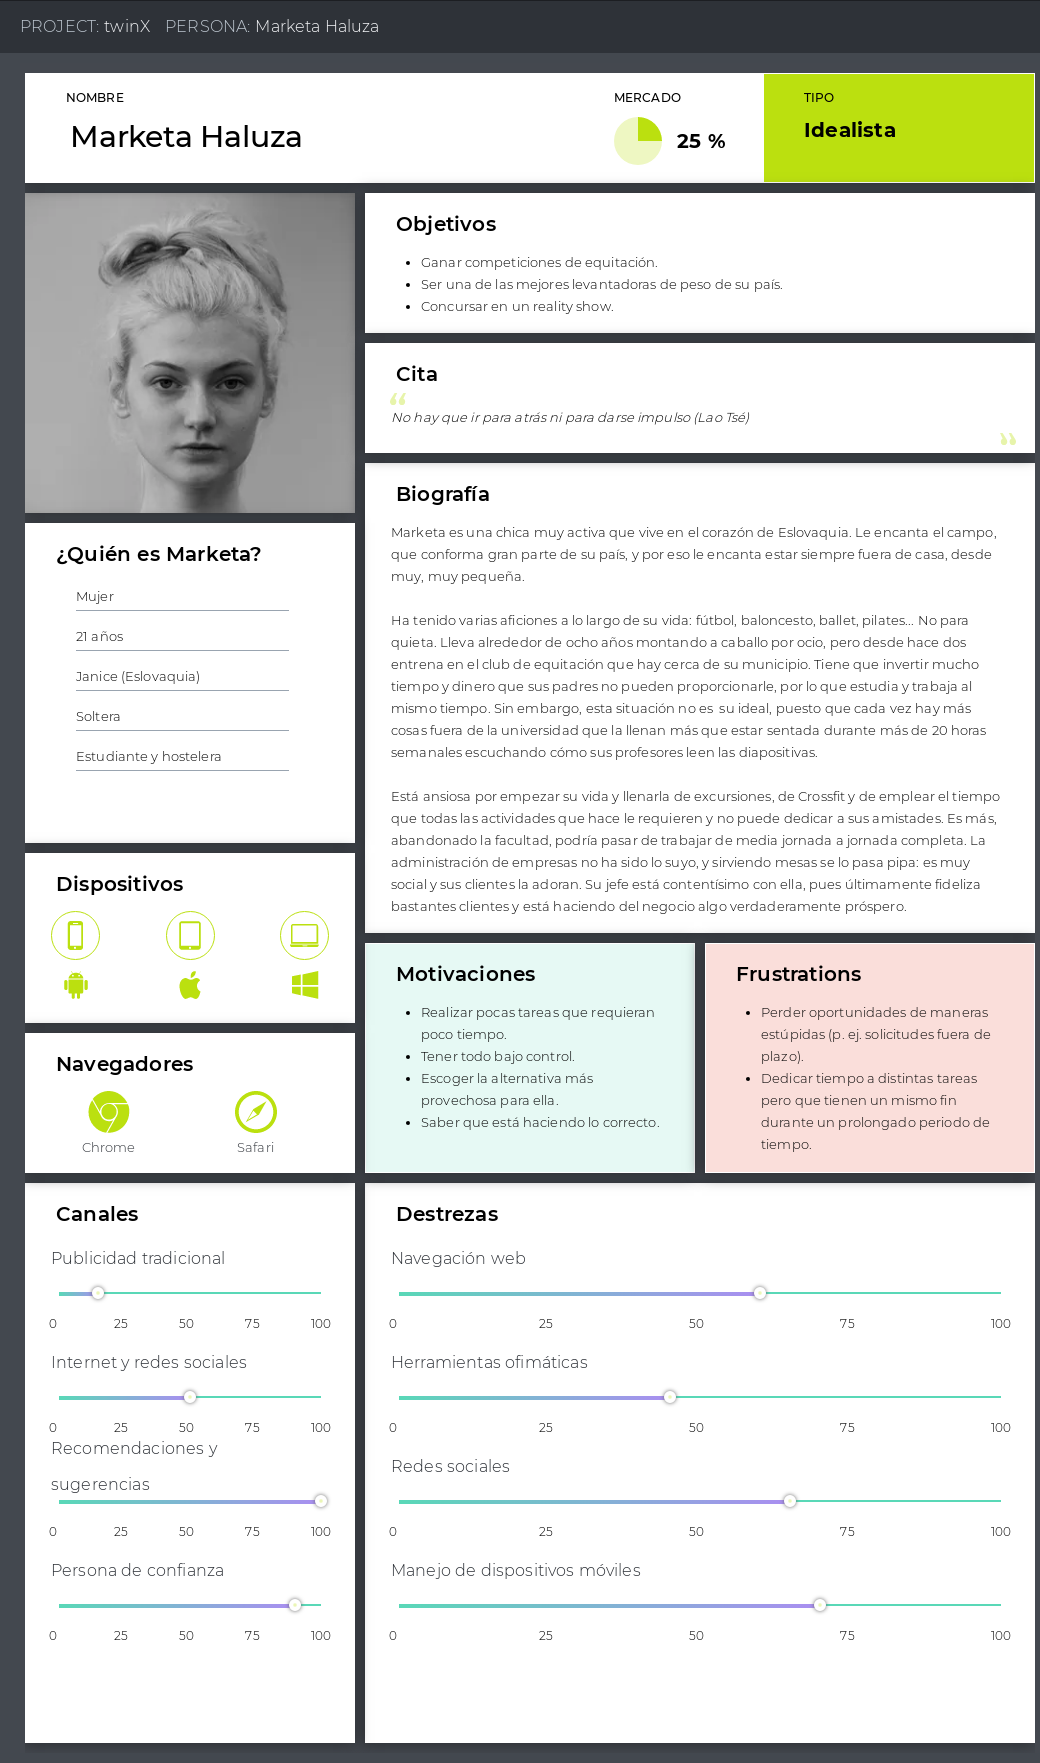
\includegraphics[width=\textwidth, height=\textheight, keepaspectratio]{img/Personas/Marketa}
	\caption[Persona \#3]{Persona \#3: Marketa}
	\label{fig:persona3}
\end{figure}

En vista de la persona en la figura \ref{fig:persona1}, Eladio, podríamos pensar que para él, lo óptimo sería desarrollar una app móvil para poder gestionar su movilidad, en caso de que quisiera hacerla. Pertenece a las nuevas generaciones donde apenas se usa el ordenador, hasta llegar a la universidad, mayormente, por lo que está acostumbrado a una tablet. Al mismo tiempo, María Gracia (figura \ref{fig:persona2}) trabaja gestionando información como la de estudiantes como Eladio o Marketa (figura \ref{fig:persona3}) y no puede permitirse interaccionar con un dispositivo móvil, pues tardaría mucho en realizar su trabajo, y no lo haría de forma efectiva. Por tanto, una solución web parece una resolución del problema apta para la mayoría del mercado del producto.

Como decíamos, nos sirven elementos que no tengan que ver directamente con las habilidades tecnológicas de los candidatos; y es que, por ejemplo, María Gracia en este caso no podría tampoco ver una web que no tuviera la tipografía lo suficientemente grande como para leer, porque podría tener la vista cansada. O quizás Marketa, si no tiene una buena situación económica, tendría quizás que conectarse desde un dispositivo algo obsoleto, por lo que probablemente le sea muy costoso en cuanto a tiempo cargar una página web con numerosas imágenes.

En definitiva, podría pensarse que los perfiles de estas tres personas están hechos para hacer el análisis de cualquier aplicación o producto software, ya que no hemos ideado estas personalidades específicamente para el problema que nos compete. Es por ello por lo que podemos tomar estos perfiles ficticios como válidos, pues no están «hechos a medida» para nosotros. Gracias a ello, podemos adaptar el desarrollo a una serie de necesidades y/o conflictos que pueden generar en otras personas al mismo tiempo, obligándonos a buscar una solución homogénea para todos, funcional y, no menos importante, que resuelva el problema como es debido y dadas las necesidades.

\section{Entrevistas}

Las reuniones con las personas que pueden entenderse como «el cliente» del producto software, han sido esenciales para el desarrollo del mismo. En primer lugar, se establecieron las bases y se definieron los problemas. Una vez lograda la comprensión, nos pusimos manos a la obra a definir cómo podríamos abordar el problema de forma que se pudiera aportar una solución de valor; si bien no definitiva y que resolviera el problema por completo, pero sí un buen comienzo como pretendemos alcanzar con este proyecto.

Como decimos, el valor de las reuniones es muy alto. Sin ir más lejos, dependía de la interacción con el creador de TWINS, Miguel Ángel Sanz, de la comprensión de los procesos implicados y de la cesión del acceso al material para la realización del proyecto. No de menos importancia son las reuniones utilizadas para la realización de pruebas, ya que durante el proceso de desarrollo el enfoque estaba en simplificar y tratar de plasmar el núcleo de TWINS para construir twinX, lo que podría llevar a futuros problemas de conceptos o de carencias no detectadas a tiempo, para lo que es fundamental el contacto con los verdaderos usuarios finales de la aplicación --o al menos en sus primeras fases--.%PENDIENTE REVISAR LO QUE SE DICE O LO QUE FALTA DE LAS ÚLTIMAS REUNIONES DE PRUEBAS

Sin estas entrevistas, hubiera sido muy complicado llegar a hacer un producto que pueda servir a la ORI-FyL, el que era un objetivo implícito, pero el cual tiene prioridad como el que más, pues de nada serviría realizar un proyecto para crear un producto que nadie pudiera llegar a utilizar. Por tanto, las aportaciones de los participantes en las entrevistas han sido los que han capacitado al desarrollo el dar como resultado una pieza de valor.

\section{Malla receptora de la información}

A las técnicas expuestas en \nameref{herramientasDT}, podemos sumar la creación de una malla que nos permita definir las partes claves de nuestro proyecto. Si bien es cierto que la \textit{Feedback Capture Grid} es mayormente utilizada para potenciar el aprendizaje tras las sesiones de pruebas, podríamos plasmar en ella los elementos que cualquier persona podría hacerse, sean o no actores que interactuarían o no con el producto final. \cite{feedbackCaptureGrid}

Su creación consiste en la división en cuatro cuadrantes de una hoja de papel, por ejemplo. En los diferentes espacios, empezando en orden de izquierda a derecha y por la parte superior, se toma nota de las buenas ideas que se han percibido tras conocer el producto, los problemas o las críticas que se le pueden encontrar, las preguntas que pueda haber y, por último, las ideas para la mejora del software que se pudieran tener, a modo de trabajos futuros.

En nuestro caso, hemos efectuado la malla (figura \ref{fig:malla}) para definir, a grandes rasgos, lo bueno que supone twinX ante TWINS, los impedimentos que tiene esta primera aproximación o proyecto piloto, las preguntas que podrían surgir por varias personas a la hora de conocer el producto (personal de administración, estudiantes, tutores...) y, por último, una serie de propuestas que se desarrollarán en la sección de trabajos futuros.


\begin{figure}
	\centering
	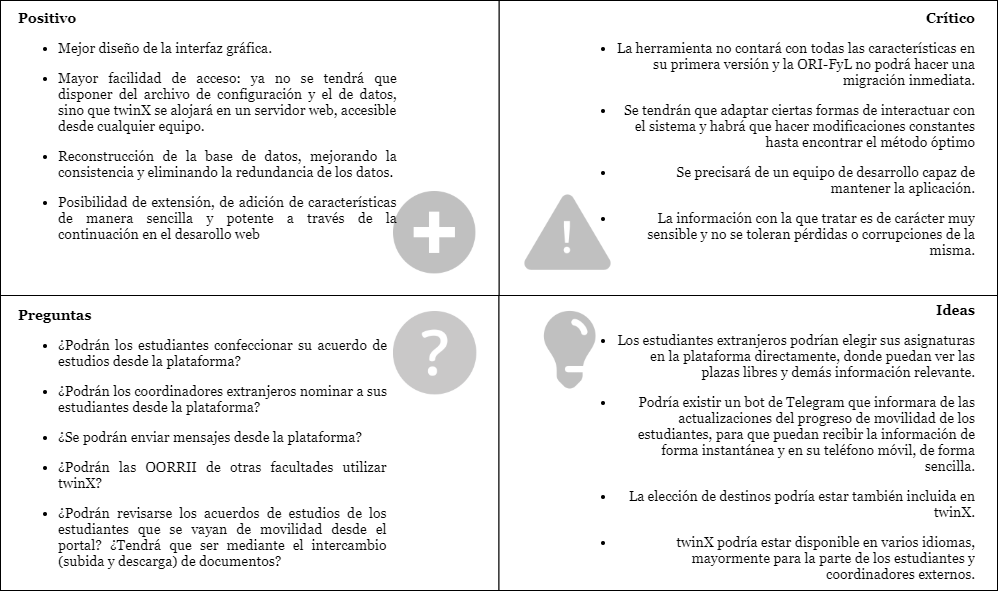
\includegraphics[width=\textwidth]{img/malla.png}
	\caption{Malla receptora de la información}
	\label{fig:malla}
\end{figure}


\section{Descripción de la propuesta}
Una vez hemos dado pinceladas de todo lo que tenemos, de qué podemos hacer, qué no y cómo llevarlo a cabo, vamos a establecer los claros objetivos de este proyecto y definir exactamente cuál será el producto tras su finalización, una vez conocemos todo el entorno que lo rodea. 

\subsection{Elección del tipo de metodología de desarrollo}
\label{elecciónMetodología}
Para desarrollar twinX primero se ha de elegir una metodología. Tradicionalmente, los proyectos de software se construían siguiendo lo que se conocen como «metodologías pesadas» o tradicionales \cite{waterfall1}, largos procesos de desarrollo en los que se definen unas fases secuenciales por donde el producto iba pasando hasta tener una versión final. La metodología más sonada es la de «cascada» o \textit{waterfall} en inglés \cite{waterfall2}. En ella, tenían lugar unas estrictas etapas enfocadas a un grupo de tareas en concreto, como son la etapa de definición, la de diseño, la de codificación, la de pruebas y la de mejora. Todo ello daba lugar a documentaciones muy completas aunque innecesariamente extensas en muchos casos, a través de la implicación de mucha gente experta en la materia, capacitada para hacer las tareas definidas muy concretamente. La flexibilidad apenas estaba contemplada, puesto que la planificación era muy estricta y hacía peligrar la buena continuidad del proyecto.

Hoy en día, apenas se utiliza este tipo de metodologías. En nuestro caso, queremos construir lo que sería tan sólo el comienzo del producto final. En otras palabras, nuestras condiciones no encajarían en una metodología en cascada, pues no tenemos unos requisitos estrictamente fijados, ya que vamos a crear una versión de TWINS no definitiva y la cual no se verá con todas las características implementadas. Además, es un cambio tan drástico el que se va a dar al transportar la aplicación a la web, que se precisa de la continua atención de una especie de «equipo supervisor», conformado por uno o varios usuarios finales del producto, que nos pueda proporcionar un \textit{feedback} sobre si nos estamos acercando o alejando de sus expectativas. Sobre esto último, diremos que no es que no se tuviera en cuenta en las metodologías tradicionales, pero no se primaba tanto como se debería, lo que hacía que el software perdiera calidad.

Por todo ello, podemos aventurarnos a decir que nuestro proyecto encaja más en una \textbf{metodología ágil}. Este tipo de metodologías se basan en la adaptación a medios con necesidades cambiantes, con un desarrollo muy de cerca con el cliente, quien está presente junto con el equipo de desarrollo en las numerosas reuniones que se hacen a lo largo de la vida del proyecto. Es más, en el \textit{14th Annual State of Agile Report} \cite{stateofagile} podemos encontrar unas estadísticas sobre los beneficios que ha traído el uso de metodologías ágiles en el último año, entre las que podemos destacar la capacidad de manejar los cambios de prioridades, la reducción de riesgos en el proyecto o el mantenimiento del software. En este caso, el equipo de desarrollo es ajustado, pero no por ello dejaremos de lado la necesaria intervención de dos personas fundamentales que hacen el papel de clientes y que son:

\begin{itemize}
	\item María Consuelo Pérez Ocaña (Coordinadora de Internacionalización en la la Facultad de Filosofía y Letras)
	\item Miguel Ángel Sanz Sáez (personal de secretaría y creador de TWINS)
\end{itemize}

\subsection{Propuesta de producto}
\label{propuesta}
En su primera versión, twinX incluirá la funcionalidad mínima de TWINS, de modo que de cara a las pruebas, la interacción con la nueva plataforma sea más bien realista, y aporte verosimilitud a la mejora, pudiendo así ser tomada como tal.

Más concretamente, contemplamos la implementación de:

\begin{itemize}
	\item El añadido, modificación y eliminación de información esencial (como son asignaturas, tipo de expediente --similar a \gls{ExpedienteTWINS}--, mensajes predefinidos, etc.)
	\item La visualización de la información relevante a estudiantes (sus datos personales, expedientes abiertos, fases de los mismos, etc.)
	\item La visualización de los \glspl{Convenio}, modificación de la información y el añadido de nuevos. Posibilidad de dos vistas: una de resumen y otra completa, tal y como se tiene en TWINS.
	\item Calendario con eventos, tareas, tal y como se disponía en TWINS
	\item El envío de mensajes, a modo de sustituir los avisos en TWINS, pero abriendo el abanico a tres tipos de mensaje: mensaje normal, recordatorio (mensaje de un usuario para sí mismo) y avisos (por proximidad a la fecha de un evento o al límite para realizar una determinada tarea).
	\item Una pantalla inicial de visualización de la información de mayor relevancia a modo de resumen. 
	\item Organización de todo el contenido en tres grandes secciones: «gestión», «calendario» y «panel de control», para simplificar y mejorar la interfaz de usuario, facilitando la interacción con la misma.
	\item Búsqueda en los distintos listados (convenios, estudiantes, expedientes...) con filtros para facilitar la recuperación de la información.
\end{itemize}

\section{Presupuesto}

\section{Planificación}
\subsection{La metodología Scrum}
En relación con la sección ~\ref{elecciónMetodología}, la metodología concreta a usar para el desarrollo de twinX será \textbf{Scrum}. Es ideal para incrementar la flexibilidad y producir un sistema que pueda responder ante tanto requisitos iniciales como los que se van añadiendo a lo largo del proceso de desarrollo que se puedan ir descubriendo.

En Scrum, se asume que el análisis, el diseño y los procesos de desarrollo son impredecibles, y por ello, tienen que ser iterativos; esto es, hay que estar constantemente comprobando el trabajo realizado, evaluando qué se ha hecho, para adaptarlo de la mejor manera posible a la situación del proyecto. Esta repetición recibe el nombre de \textbf{sprint}, y es una medida de esta metodología.

Los sprints son flexibles y no lineales. Se podrían tomar como una caja negra que precisa de controles externos. De este modo, en cada iteración se pueden tener en cuenta todos los factores que se crean necesarios, de forma que se evite convertir el proceso en algo caótico y que se aleje de los objetivos del proyecto y, al mismo tiempo, se pueda maximizar la flexibilidad. \cite{scrum}

Vamos a agrupar en tres bloques las fases de la metodología Scrum:
\begin{itemize}
	\item \textbf{Preparación.} Podemos diferenciar dos subfases:
	\begin{itemize}
		\item Planificación: donde se estiman el coste y el tiempo del proceso
		\item Arquitectura: para decidir cómo se van a implementar los elementos de la lista de trabajos pendientes o \textit{backlog}
	\end{itemize} 
	\item \textbf{Desarrollo:} donde se lleva a cabo la realización de los sprints acordados en la fase anterior. Se desarrollan nuevas funcionalidades, respetando las variables del tiempo, requisitos, calidad, coste y competición. El fin de esta fase está condicionado a cuán bien se interacciona con las variables mencionadas.
	\item \textbf{Finalización:} preparación para el lanzamiento del producto, donde se incluye la documentación final, y unas pruebas que se realizan con anterioridad a la versión final del software.
\end{itemize}

\subsection{Planificación en sprints}

A continuación, vamos a exponer la planificación que se ha pensado para llevar a cabo el desarrollo de este producto piloto para la plataforma twinX, de acuerdo con lo expuesto en la sección ~\ref{propuesta}:

\subsubsection*{\textbf{Sprint 0: puesta a punto}}

\begin{itemize}
	\item \textbf{Toma de decisiones acerca del renombramiento de algunas entidades existentes en TWINS:} existen una serie de nombres que pueden ser confusos para una persona que trate de comprender el funcionamiento de TWINS desde cero; si bien esto no ocurre con los usuarios habituales de la aplicación de Access\textregistered, con el desarrollo de twinX estamos, por lo general, facilitando a todo el entorno de la ORI-FyL, y por tanto, se renombrará alguna entidad como por ejemplo «evento». El motivo no es otro que la confusión entre un evento de calendario cotidiano y un \gls{EventoExpedienteTWINS}. Para ello, se tiene que hacer un segundo análisis de la base de datos ya creada y así poder mejorar la comprensión de nuevos usuarios en la plataforma.
	\item \textbf{Realización de un tutorial de \textit{Yii2 Framework}:} sobre los detalles de la tecnología a usar para el desarrollo de twinX hablaremos en la sección ~\ref{implementacion}. Sin embargo, antes de ponernos manos a la obra con la implementación del sistema web, habrá que adquirir los conocimientos necesarios para la toma de buenas decisiones y el respeto de las buenas prácticas del framework. %PENDIENTE
	\item \textbf{Modelado de la base de datos:} realizar el diseño lógico-conceptual de la base de datos es esencial a la hora del desarrollo. Una vez se tiene, podemos crear las tablas necesarias para hacer funcionar la aplicación. Es de suma importancia dedicar el tiempo suficiente a esta tarea, dado que los  errores en el modelo pueden dar lugar a imprevistos temporales en el futuro.
	\item \textbf{Creación de bocetos:} necesarios para confeccionar las interfaces de usuario sobre un esquema ya pensado, de modo que las decisiones de diseño de importancia tengan lugar en esta fase, y no sobre la marcha, ya que es más costoso en cuanto a tiempo y la consistencia de las vistas puede verse comprometida.	
\end{itemize}


\subsubsection*{\textbf{Sprint 1: comienzo del desarrollo}}

\begin{itemize}
	\item \textbf{Integrar el \gls{paneltwinX}:} desde donde se añadirán nuevos registros a la plataforma, del lado del \gls{superusuario}. Es la parte más importante si tenemos en cuenta que es la que nos posibilita hacer pruebas de la manera más sencilla, ya que no se espera que twinX tenga en su primera versión ninguna herramienta de migración masiva de datos. 
	%PARA LA SECCIÓN 4
%	\begin{itemize}
%		\item \textbf{Integrar la vista de usuarios}	
%		\item \textbf{Integrar la vista de fases de expediente}
%		\item \textbf{Integrar la vista de mensajes predefinidos}
%		\item \textbf{Integrar la vista de países}
%		\item \textbf{Integrar la vista de universidades}
%	\end{itemize}

	\item \textbf{Integrar el módulo de \gls{gestiontwinX}:} como parte fundamental de twinX, donde se tiene la mayor parte de la funcionalidad y las acciones que los \glspl{gestortwinX} llevarán a cabo durante su jornada laboral a diario, pues viene siendo el corazón del actual TWINS.
	%PARA LA SECCIÓN 4
%	\begin{itemize}
%		\item \textbf{Integrar la vista de convenios}	
%		\item \textbf{Integrar la vista de asignaturas}
%		\item \textbf{Integrar la vista de estudiantes}
%		\item \textbf{Integrar la vista de expedientes}
%		\item \textbf{Integrar la vista de tutores}
%	\end{itemize}
	
\end{itemize}

\subsubsection*{\textbf{Sprint 2: complementando twinX}}

\begin{itemize}
	\item \textbf{Integración del módulo de calendario:} el cual tendrá los mismos elementos que el calendario en TWINS, con eventos, tareas asociadas a los mismos, y avisos, en forma de mensaje, para las fechas límite de las tareas.
	\item \textbf{Integración del módulo de mensajería:} para el intercambio de mensajes o notas, en sustitución del confuso menú de la figura \ref{fig:avisos}
\end{itemize}

\subsubsection*{\textbf{Sprint 3: ensanchando horizontes}}

\begin{itemize}
	\item \textbf{Integrar el \textit{frontend} del estudiante:} con acciones básicas como el registro y la confección del acuerdo de estudios.
	\item \textbf{Integrar el \textit{frontend} del tutor:} para interaccionar con sus estudiantes y poder revisar sus acuerdos de estudios.
\end{itemize}

\subsubsection*{\textbf{Sprint 4: haciendo twinX aún más potente}}

\begin{itemize}
	\item \textbf{Integración del reconocimiento de créditos:} para los estudiantes salientes, trasladar sus puntuaciones obtenidas en su universidad de destino a calificaciones ponderables en su expediente en la UGR.
	\item \textbf{Integración de la alteración de matrícula:} proceso mediante el cual los estudiantes entrantes pueden tener asignadas sus asignaturas, confeccionados sus horarios dependiendo de factores como las plazas vacantes o el posible solapado de clases en un tramo horario.
	\item \textbf{Funcionalidad de migración de datos masiva:} desde la sede de la UGR, quien comunica a la ORI-FyL los listados de los estudiantes de movilidad entrantes y salientes.
\end{itemize}

Todas estas tareas pueden ser, acorde con la metodología Scrum, modificadas y trasladadas a otros sprints. Sobre las subtareas que conllevaría cada épica\footnote{Las épicas son tareas que almacenan dentro de ellos un gran número de subtareas.} (las expuestas anteriormente), hablaremos en la sección ~\ref{diseñoTécnico}. %PENDIENTE

Independientemente de la división del trabajo en todos estos sprints, no se contempla la realización de más de uno o dos de ellos, con la posibilidad de cambiar los contenidos de los mismos, pues también habría que incluir la realización de las pruebas y la redacción de esta memoria.

En adición a la planificación aquí expuesta, cabe señalar la utilización de un tablero \textbf{Kanban}, característico de las metodologías ágiles y de Scrum. En él, se disponen las tareas en varias columnas. A cada tarea se le puede asignar un color para distinguirlo, por ejemplo, en los distintos sprints. Para la construcción de twinX hemos usado la herramienta \textit{Trello} para la confección de un tablero interactivo (figura \ref{fig:kanban}). Las distintas etiquetas representan distintos sprints, y a cada tarea (consideradas en su mayoría como épicas), se les puede adjuntar una lista de tipo \textit{checkbox} para asegurarnos de que no queda tarea sin hacer dentro de cada épica.

\begin{figure}
	\centering
	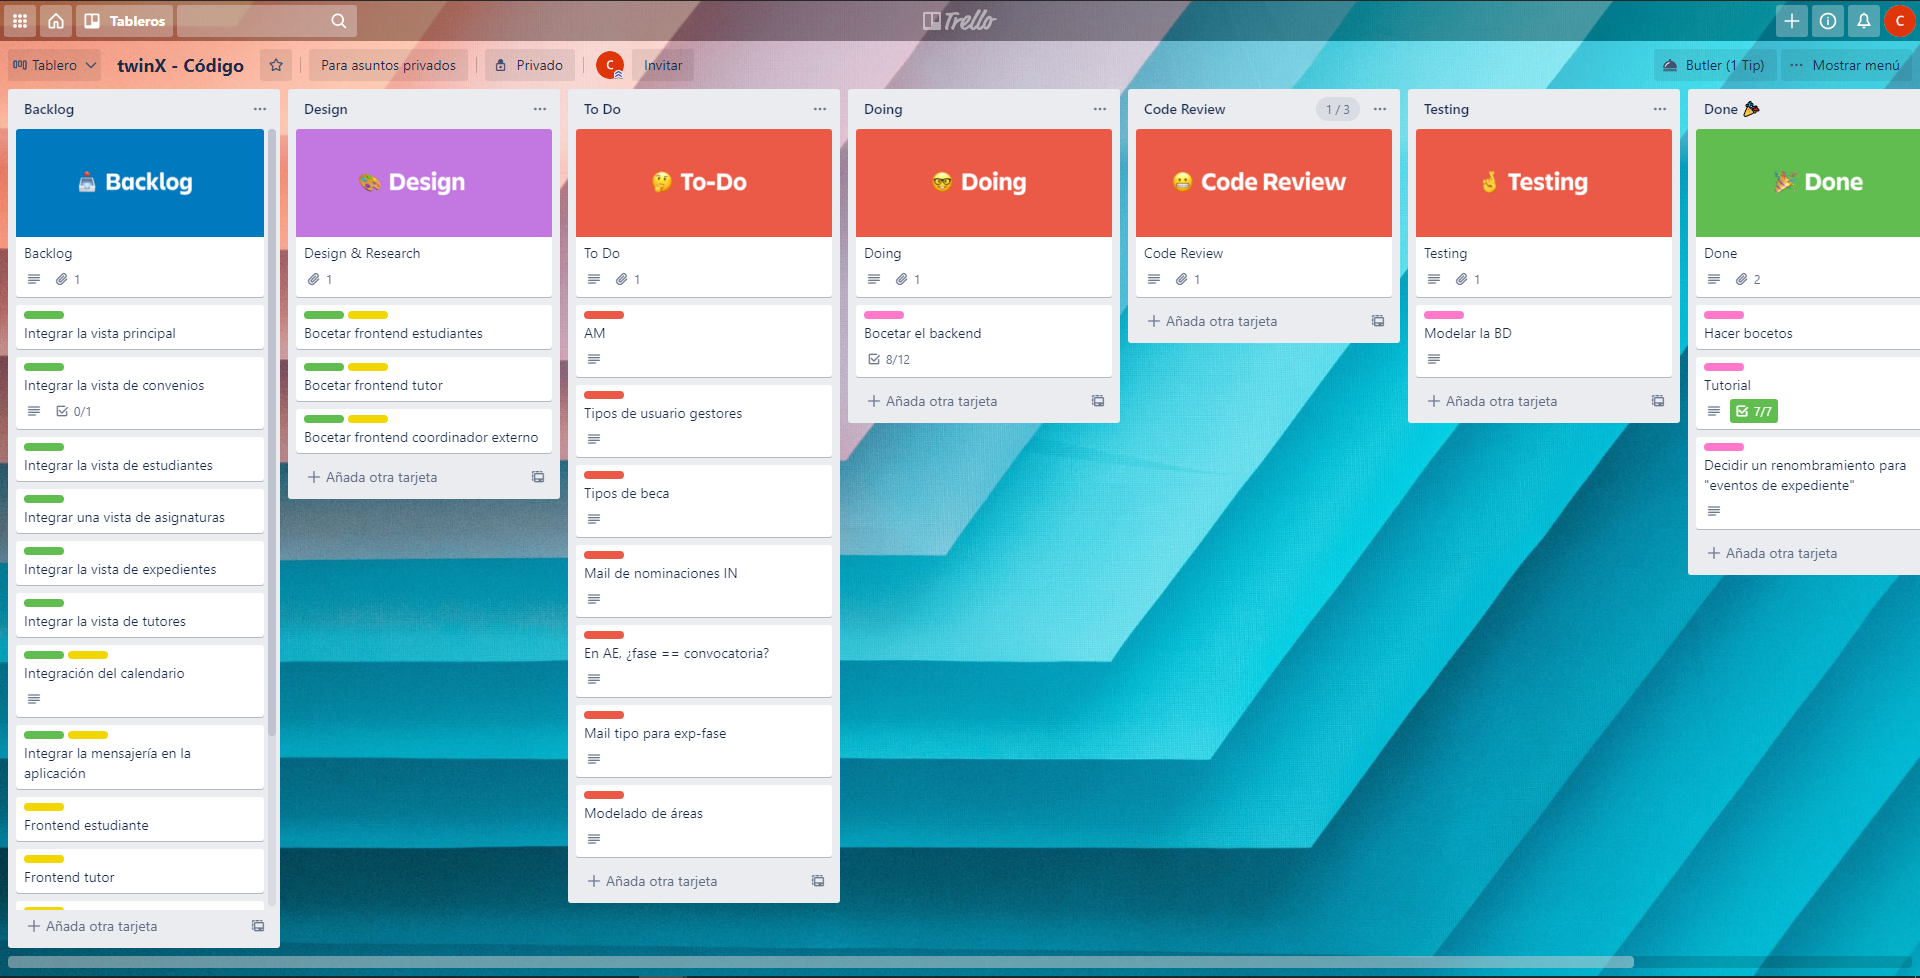
\includegraphics[width=\textwidth]{img/Capturas Kanban/kanban_codigo}
	\caption{Kanban al comienzo del desarrollo}
	\label{fig:kanban}
\end{figure}



% 4. Diseño de la interfaz de usuario

\chapter{Diseño de la interfaz de usuario}

Una vez hemos definido cuáles son nuestros objetivos, analizado el estado del arte y establecido unas pautas para el desarrollo, vamos a comenzar con el diseño de la parte visual. Esto es, a su vez, un proceso que requiere de distintas definiciones, de manera que al término de este capítulo, no sólo tengamos el diseño de las interfaces de usuario, sino que también comprendamos por qué se han diseñado así y la intención de cada elemento que disponemos en pantalla.

\section{Matriz de tareas de usuario}

Un buen comienzo sería el de definir los roles de usuario en nuestra nueva aplicación. Hemos hablado ya en el capítulo anterior sobre la figura del \gls{gestortwinX} y la del \gls{administradortwinX}. Incluyamos entonces también las de \gls{Tutor}, estudiante y, de forma excepcional, la de coordinador(a) externo/a. Sobre esta última, recordemos que no tenía ningún tipo de interacción en TWINS y que hasta entonces, los usuarios de la plataforma habían establecido intercambios de información por correo electrónico con los coordinadores de otras facultades, que es el método estándar de realizar las \glspl{Nominacion}. Sin embargo, aunque no para sus primeras versiones, se espera que twinX brinde la capacidad de hacer estas nominaciones a través de una interfaz gráfica, de una forma mucho más sencilla y segura que con el envío de un texto libre, donde puede haber errores y/o malas prácticas, dado el amplio uso que se puede hacer de la herramienta.

Es precisamente por la necesidad de dejar claras las acciones a llevar a cabo por cada usuario del sistema por la que elaborar una \textbf{matriz de tareas de usuario}. Esta herramienta nos permite establecer cuál es la frecuencia de uso de una característica de nuestra aplicación por un grupo de usuarios en concreto y cuál es la prioridad que debemos darle a la implementación de la misma. De esta forma, nos será más fácil diferenciar aquellas acciones que tan solo se lleven a cabo unas pocas veces al mes (o cada varios meses) y cuales, por el contrario, son ejecutadas casi a diario, de modo que se priorice su integración y su optimización. Sobre estas últimas, cabe decir que el potenciarlas no solo se procurará hacer en términos de procesamiento interno del código, sino también en cuanto a su facilidad de utilización por parte del usuario. Es decir, tendremos que crear más accesos directos o simplificar lo máximo posible el curso de tareas a llevar a cabo para realizar estas acciones y obtener los resultados deseados. En adición a todo esto, podremos observar cuáles son los usuarios que menos usarán la plataforma, de modo que se reste prioridad a la implementación de sus interacciones, en beneficio de las que llevan a cabo los usuarios que, por el contrario, monopolizan el uso de la aplicación. \cite{matrizTareas}

Para simplificar la matriz (tabla \ref{tab:matrizTareas}) y hacerla visualmente más sencilla de entender, vamos a asignar una serie de letras que correspondan a un nivel de utilización en concreto. Elegiremos la «A» para una frecuencia de uso alta, «M» para un uso medio y «B» para una baja frecuencia. A estas indicaciones añadiremos unas puntuaciones que nos permitirán determinar con mayor facilidad cuáles son las tareas de mayor importancia y cuáles son menos urgentes de implementar, al igual que los usuarios que desempeñarán un papel más o menos crítico en la aplicación. Respectivamente serán 3, 2 y 1 punto, de modo que las prioridades más altas recibirán una mayor puntuación y viceversa.

\begin{table}[h]
	\begin{center}
		\begin{adjustbox}{width=1\textwidth}
		\begin{tabular}{ | >{\centering\arraybackslash}p{0.375\linewidth} | c | c | c | c | c | c | } 
			\hline
			\textbf{Usuarios / Tareas} & \textbf{Administrador} & \textbf{Gestor} & \textbf{Tutor} & \textbf{Estudiante} & \textbf{Coordinador externo} & \textbf{Puntuación} \\
			\hline
			Acceder a twinX & M & A & B & B & B & \cellcolor{red!25}8 \\
			\hline
			Ver expedientes de un usuario & A & A & & & & \cellcolor{red!25}6 \\
			\hline
			Cambiar de fase un expediente & A & A & & & & \cellcolor{red!25}6 \\ 
			\hline
			Consultar la información de un convenio & A & A & & & & \cellcolor{red!25}6 \\ 
			\hline
			Modificar los datos de un estudiante & M & M & & B & & \cellcolor{red!25}5 \\
			\hline
			Introducir un nuevo convenio & B & M & & & & 3 \\
			\hline
			Realizar el acuerdo de estudios & & & & B & & 1 \\
			\hline
			Revisar propuesta de acuerdo de estudios & & B & M & & & 3 \\
			\hline
			Consultar los expediente pendientes de procesamiento & M & A & & & & 5 \\
			
			\hline
			Expresar consentimiento de cesión de datos & & & & B & & 1 \\
			\hline
			Añadir un nuevo tipo de expediente y/o fase de expediente & B & & &  & & 1 \\
			\hline
			Marcar un expediente como favorito & B & M & & & & 3 \\
			\hline	
			\textbf{Puntuación del grupo de usuarios} & \cellcolor{red!25}18 & \cellcolor{red!25}22 & 3 & 4 & 1 &  \\
			\hline
	\end{tabular}

	\end{adjustbox}
		\caption{Matriz de tareas de usuario}
		\label{tab:matrizTareas}
	\end{center}
\end{table}

Tras la atenta observación de la matriz, podemos afirmar que las acciones que mayor uso van a tener por los usuarios de twinX serían las ya existentes en TWINS, como es lógico, y que por supuesto, los grupos de usuarios con mayor necesidad de uso de la aplicación son los gestores y administradores. Sobre éstos últimos, cabe señalar que son una especie de gestores con más permisos de lo normal, de modo que pueden modificar la información que clasifica la situación de los estudiantes como son, por ejemplo, las fases de los expedientes. Solo los administradores podrían hacerlo, ya que los gestores no tienen por qué tener acceso a dichas modificaciones; simplemente necesitan trabajar con las ya registradas y, en caso de necesitar más entradas o la modificación de otras existentes, tendrían que solicitarlo a los administradores.

Con esta matriz, además, justificamos que el contenido de la primera versión de twinX (descrito en la sección ~\ref{propuesta}), es suficiente para cubrir la mayoría de las necesidades esenciales del trabajo de un secretario de la ORI-FyL, lo que es uno de los objetivos principales de este proyecto, aunque sea tan solo un comienzo a lo que finalmente llegaría a ser twinX.

\section{Sitemap}
\section{Labelling (iconografía)}
\section{Bocetos wireframe}

\subsection{Wireframes del módulo de gestión}

\begin{figure}
	\centering
	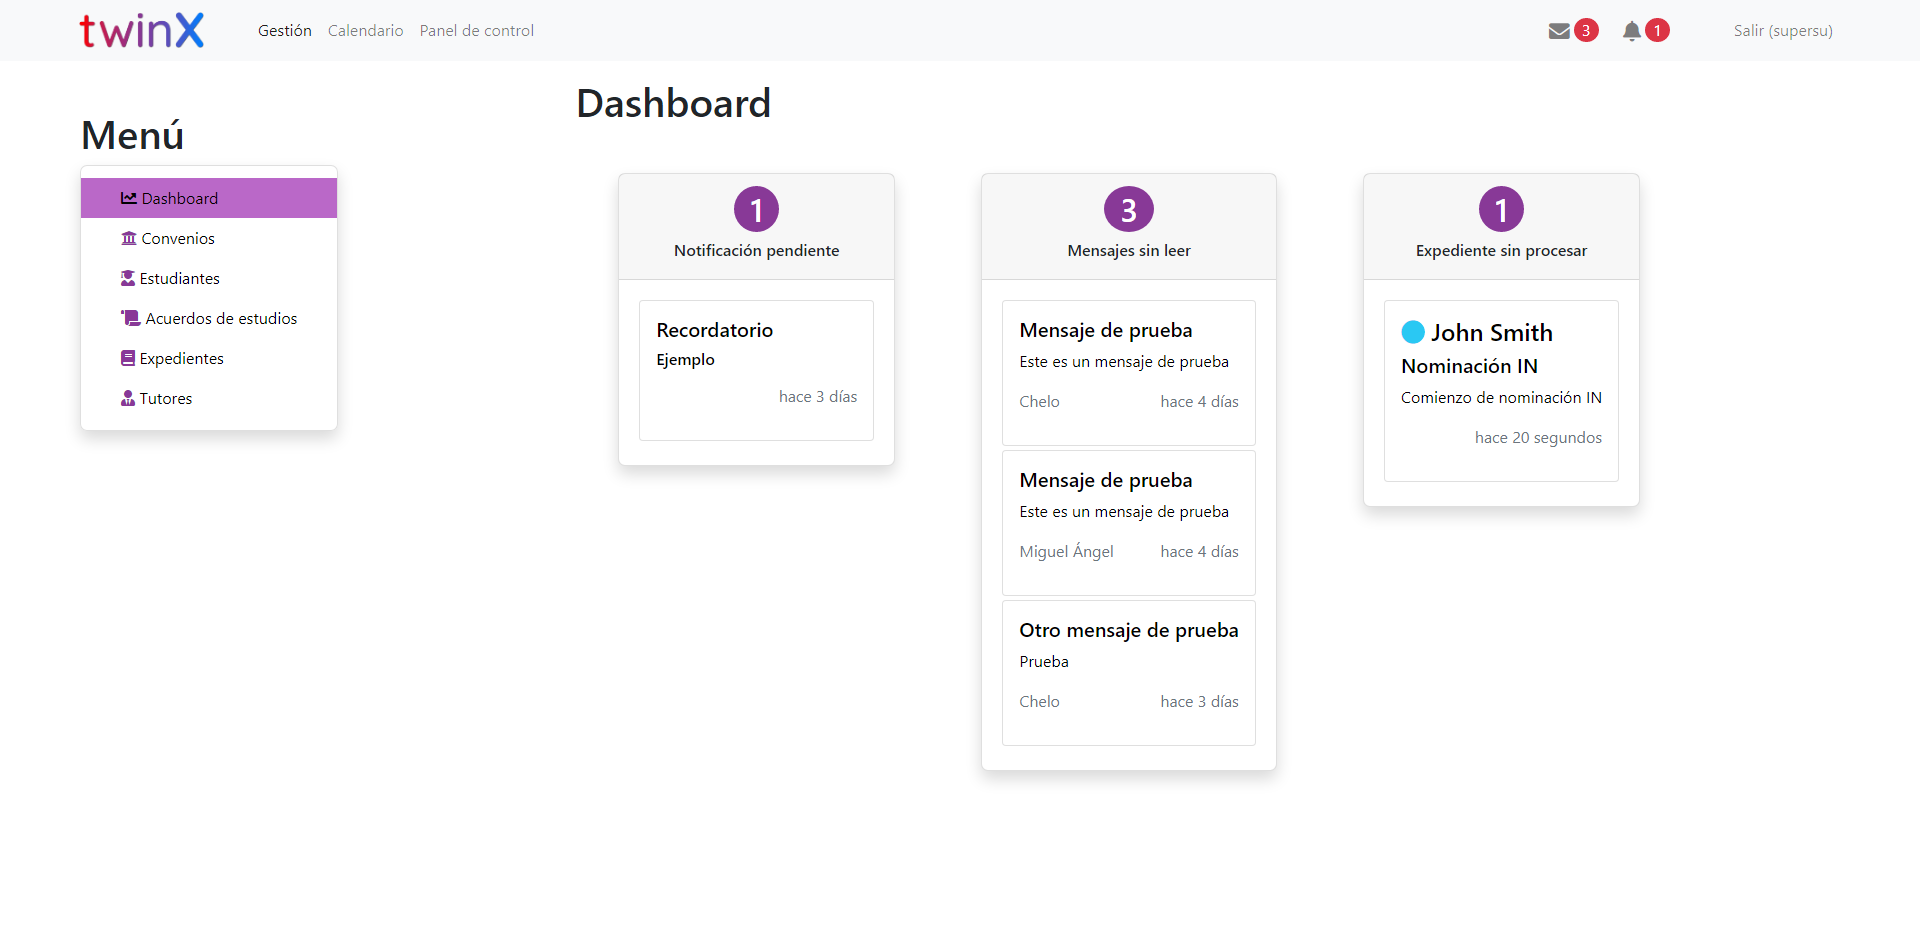
\includegraphics[width=\textwidth]{img/Wireframes/Gestión/dashboard.png}
	\caption[Wireframe de \textit{Dashboard}]{Wireframe del \textit{Dashboard} donde el usuario verá de un vistazo toda la información de mayor importancia al iniciar la aplicación}
	\label{fig:dashboardWF}
\end{figure}

\begin{figure}
	\centering
	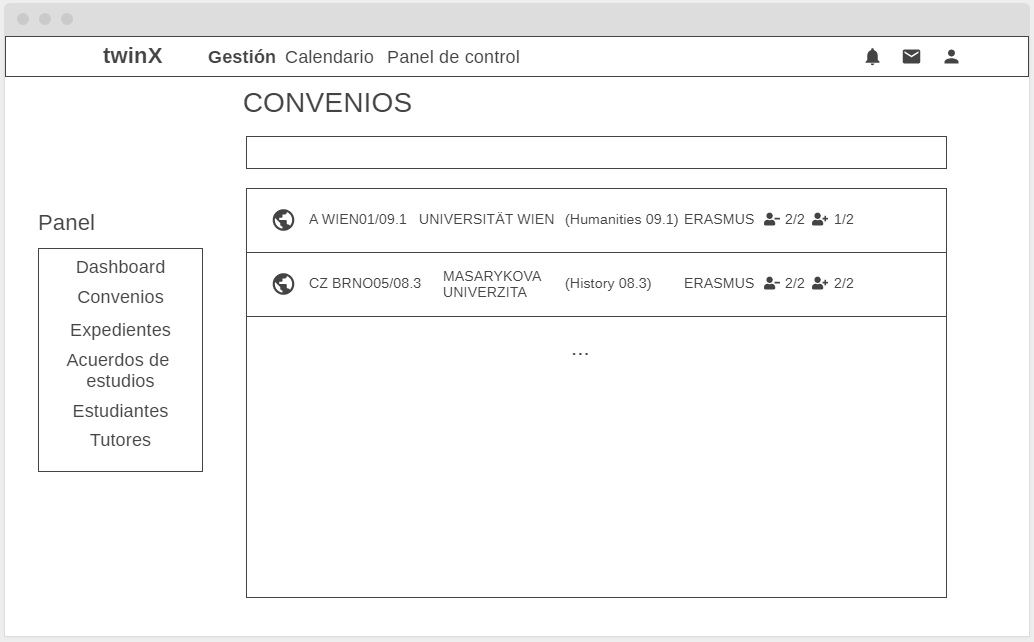
\includegraphics[width=\textwidth]{img/Wireframes/Gestión/convenios_lista.png}
	\caption{Wireframe de lista de convenios}
	\label{fig:convenios_listaWF}
\end{figure}

\begin{figure}
\centering
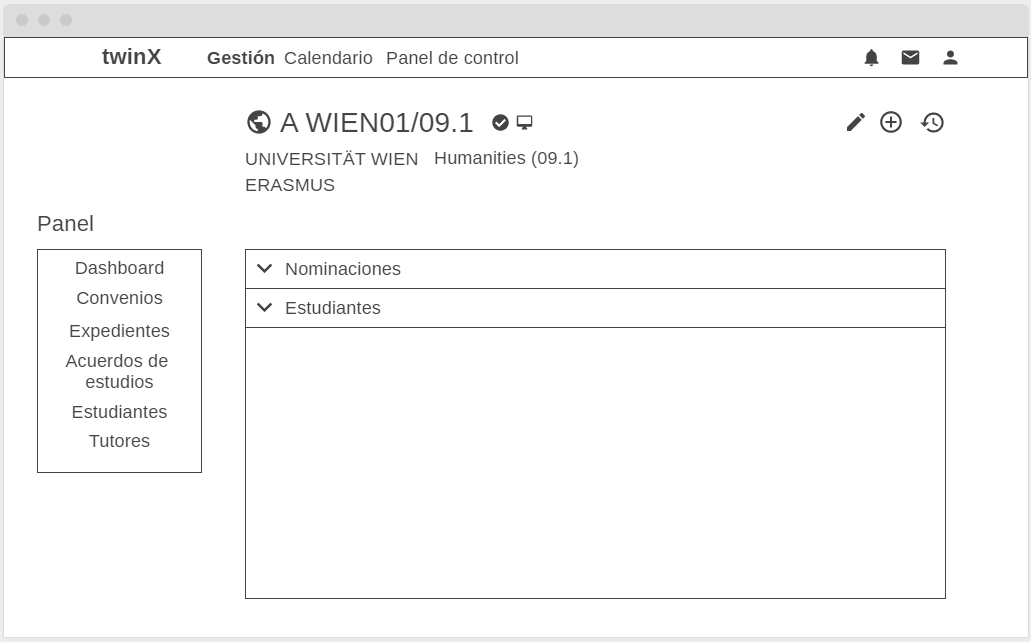
\includegraphics[width=\textwidth]{img/Wireframes/Gestión/vista_convenio_básica_contraída.png}
\caption[Wireframe de vista de convenio básica]{Wireframe de vista de convenio básica. Secciones contraídas.}
\label{fig:vista_conv_básica_contWF}
\end{figure}

\begin{figure}
	\centering
	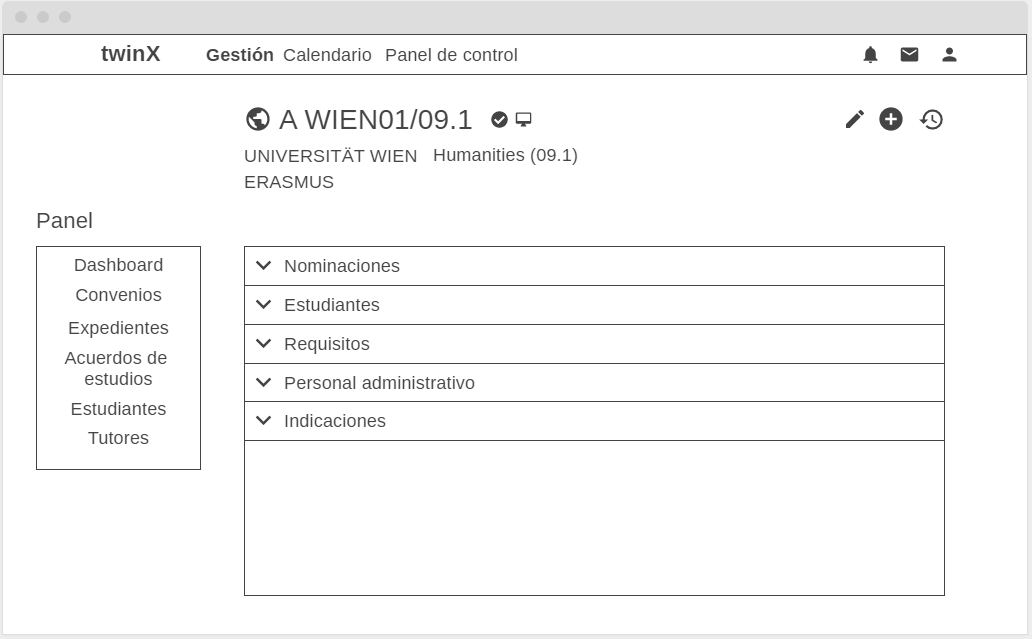
\includegraphics[width=\textwidth]{img/Wireframes/Gestión/vista_convenio_avanzada_contraída.png}
	\caption[Wireframe de vista de convenio avanzada]{Wireframe de vista de convenio avanzada. Secciones contraídas. Acceso desde el botón «+» de la botonera en la esquina superior derecha del contenido principal.}
	\label{fig:vista_conv_avanzada_contWF}
\end{figure}

\begin{figure}
	\centering
	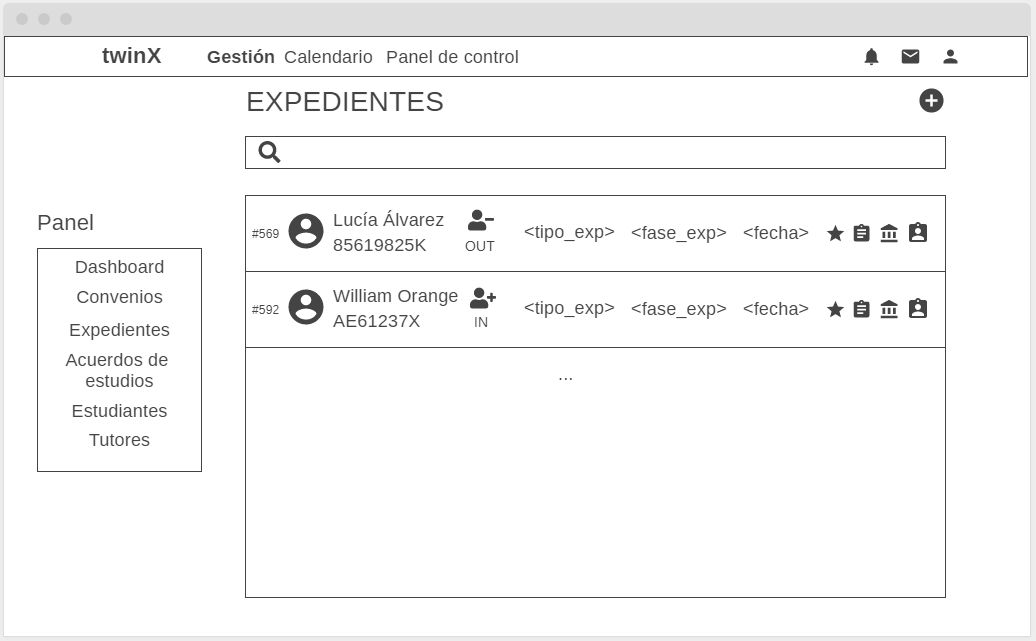
\includegraphics[width=\textwidth]{img/Wireframes/Gestión/expedientes_lista.png}
	\caption{Wireframe de lista de expedientes}
	\label{fig:expedientes_listaWF}
\end{figure}

\begin{figure}
	\centering
	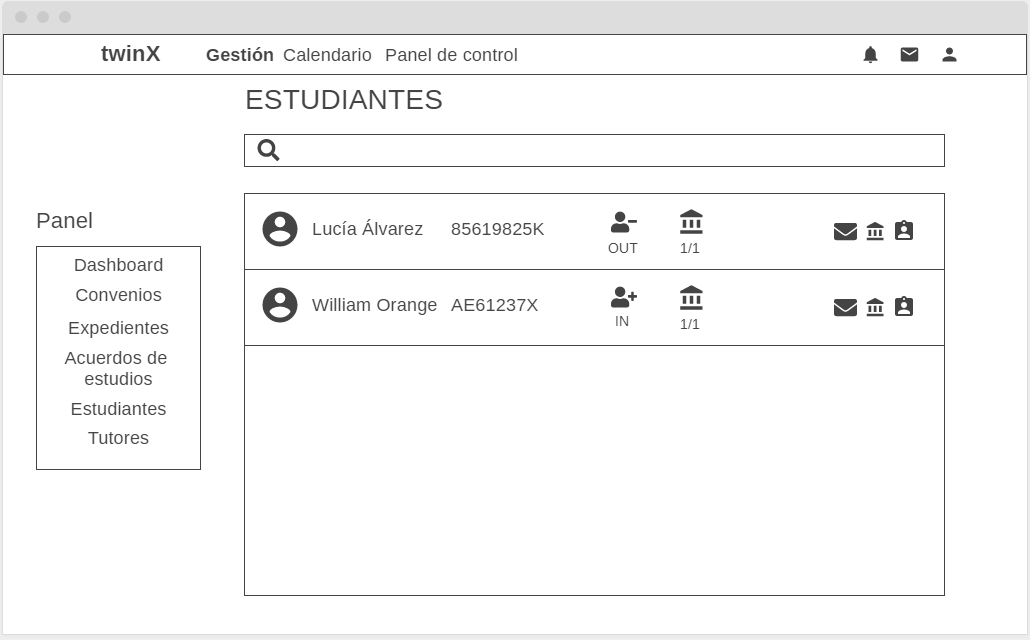
\includegraphics[width=\textwidth]{img/Wireframes/Gestión/estudiantes_lista.png}
	\caption{Wireframe de lista de estudiantes}
	\label{fig:estudiantes_listaWF}
\end{figure}

\begin{figure}
	\centering
	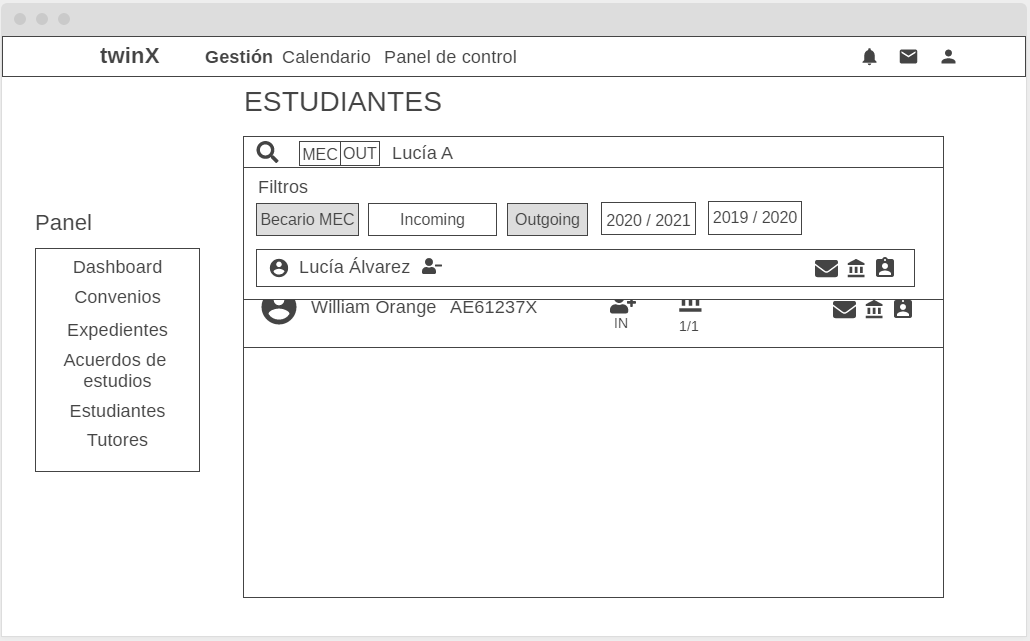
\includegraphics[width=\textwidth]{img/Wireframes/Gestión/búsqueda.png}
	\caption[Wireframe de búsqueda]{Wireframe de búsqueda. Diálogo modal, desplegable desde la barra. Capacidad de filtrado}
	\label{fig:búsquedaWF}
\end{figure}

\begin{figure}
	\centering
	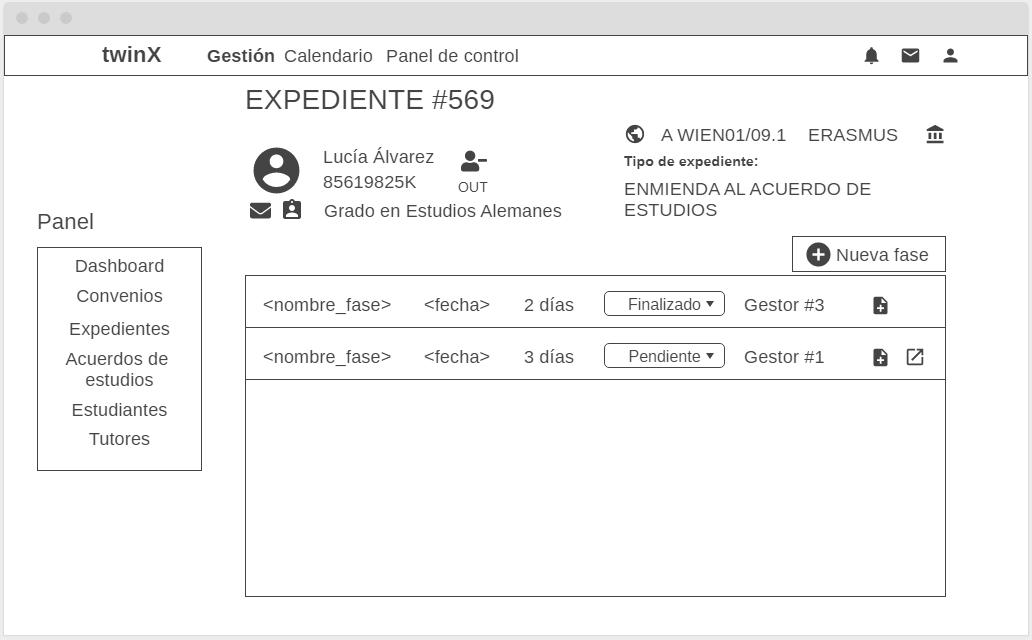
\includegraphics[width=\textwidth]{img/Wireframes/Gestión/expediente_detalle.png}
	\caption{Wireframe de detalle de expediente}
	\label{fig:expediente_detalleWF}
\end{figure}

\begin{figure}
	\centering
	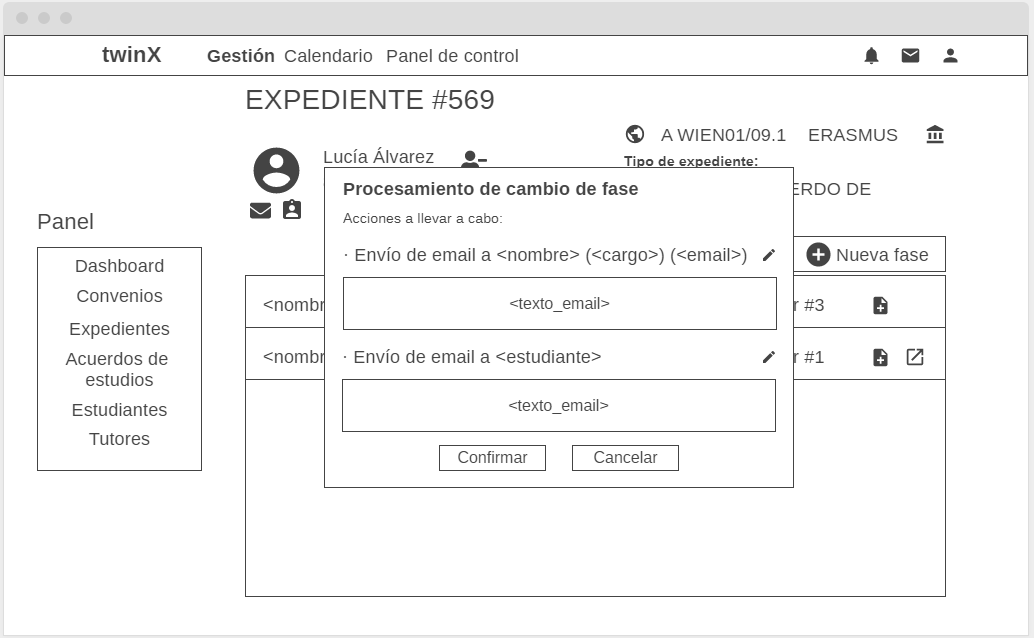
\includegraphics[width=\textwidth]{img/Wireframes/Gestión/cambio_fase.png}
	\caption[Wireframe del modal de cambio de fase]{Wireframe del modal de cambio de fase. Advierte sobre las acciones a llevar a cabo tras la tramitación del cambio de fase en un expediente concreto.}
	\label{fig:cambio_faseWF}
\end{figure}

\begin{figure}
	\centering
	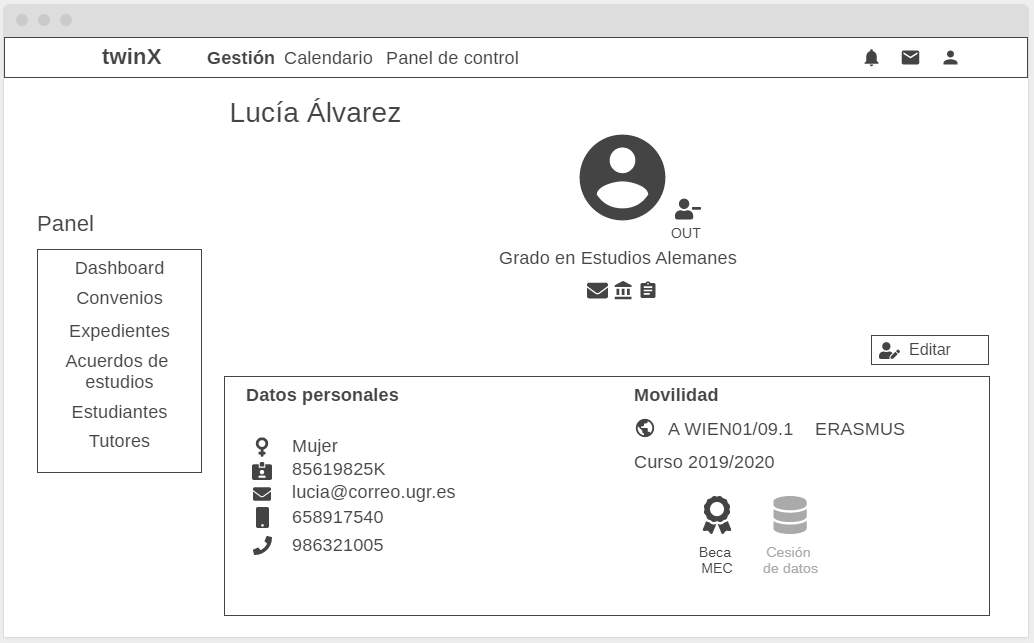
\includegraphics[width=\textwidth]{img/Wireframes/Gestión/estudiante_detalle.png}
	\caption{Wireframe de la vista de detalle de un estudiante}
	\label{fig:estudiante_detalleWF}
\end{figure}

%%PROVISIONAL PARA SEPARAR AMBOS CONJUNTOS DE WIREFRAMES
\newpage

\subsection{Wireframes del módulo de calendario}

\begin{figure}
	\centering
	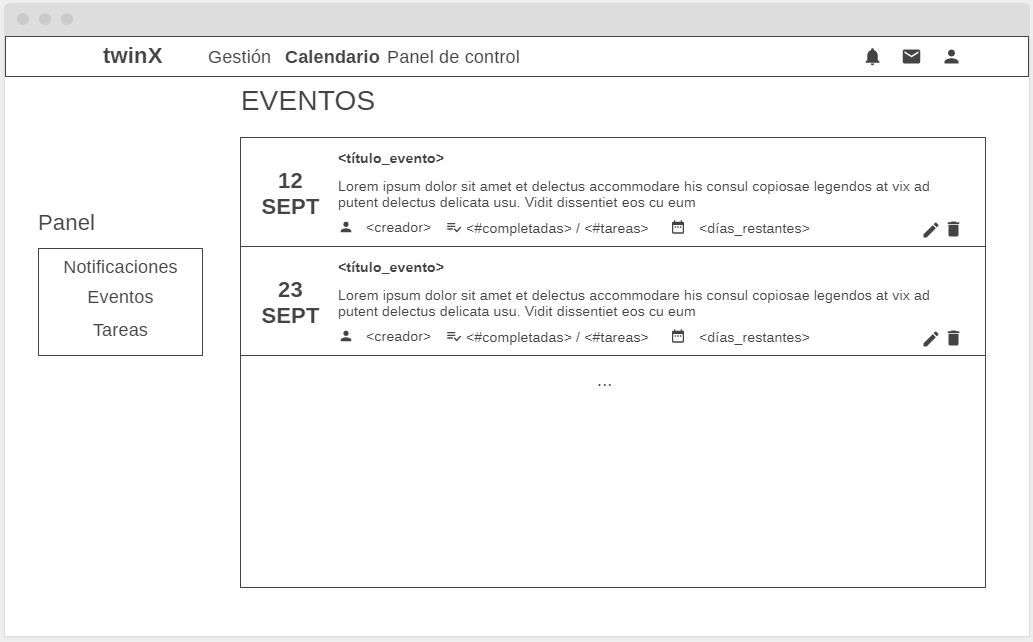
\includegraphics[width=\textwidth]{img/Wireframes/Calendario/eventos_lista.png}
	\caption{Wireframe de lista de eventos}
	\label{fig:eventos_listaWF}
\end{figure}

\begin{figure}
	\centering
	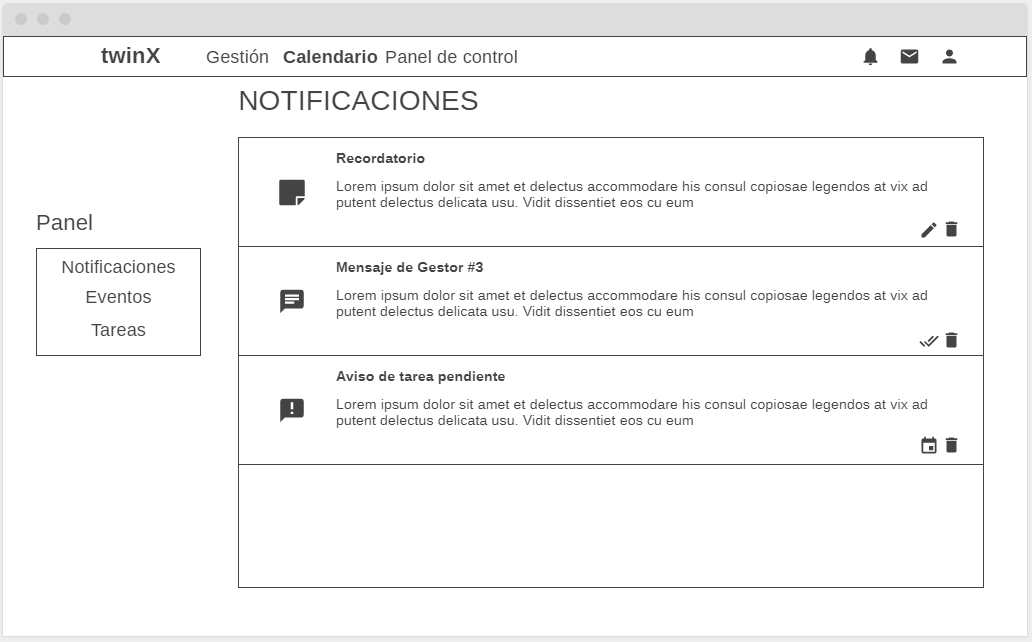
\includegraphics[width=\textwidth]{img/Wireframes/Calendario/notificaciones_lista.png}
	\caption[Wireframe de lista de notificaciones]{Wireframe de lista de notificaciones. Pueden aparecer tres tipos de notificaciones, dependiendo del tipo de mensaje recibido o generado por la propia plataforma (a través de avisos y/o recordatorios)}
	\label{fig:notificaciones_listaWF}
\end{figure}

\begin{figure}
	\centering
	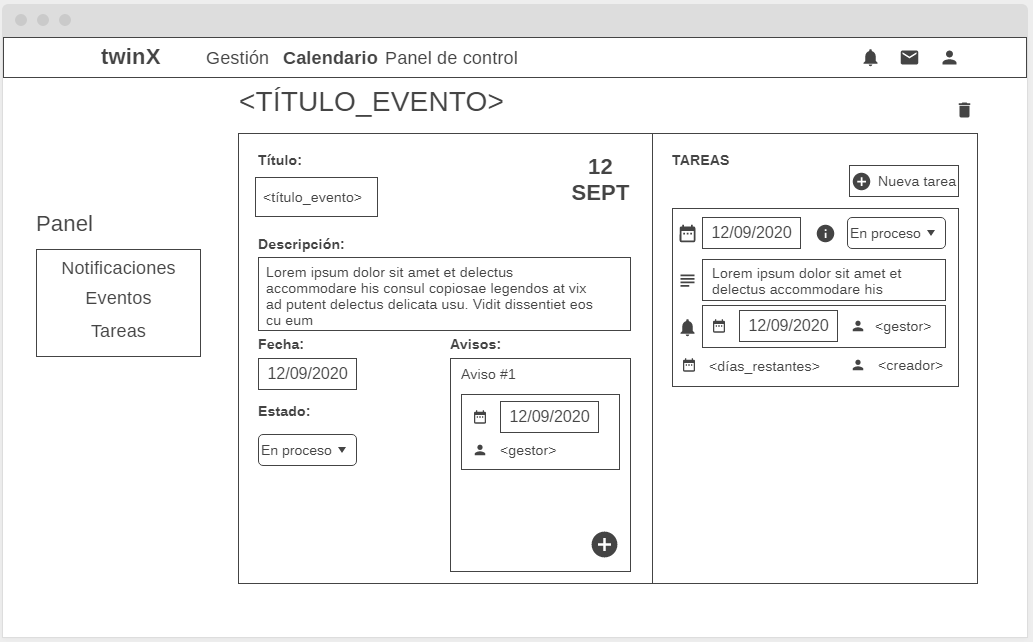
\includegraphics[width=\textwidth]{img/Wireframes/Calendario/nuevo_evento.png}
	\caption[Wireframe de creación de un evento]{Wireframe de creación de un evento. Se distinguen dos vistas: la información del evento en general (izquierda) y la de sus subtareas (derecha)}
	\label{fig:nuevo_eventoWF}
\end{figure}





% 4. Diseño técnico

\chapter{Diseño técnico}

Hemos definido hasta ahora gran parte de los ingredientes que llevará twinX: quiénes lo van a usar, qué es capaz de hacer, cuánto vamos a tardar en hacerlo y por qué hace falta algo como twinX.

Es hora de ponernos manos a la obra. Pero antes de ello, es necesario aún definir muchas más cosas, todo ello en relación con lo anterior pero a más bajo nivel: cuáles van a ser exactamente nuestras tareas, qué subtareas asociadas tendremos que desarrollar y cómo va a ser la base de datos. Será vez puestos todos los ingredientes a nuestra disposición para cocinarlos cuando podamos comenzar a utilizar nuestras herramientas para conseguir nuestro objetivo.

\section{Listado inicial del producto (product backlog)}

Es cierto que ya sabemos lo que va a ser capaz de hacer twinX en su primera versión, pero no tenemos claros los pequeños pasos a dar para poder completar las grandes tareas que ya conocemos. Por ello, vamos a elaborar un listado de todo lo que tenemos que hacer en orden de preferencia, paso a paso, para poder conseguir nuestros objetivos de manera organizada.

La priorización de la lista de tareas suele estar hecha por el llamado \textit{product owner}; esto es, el propietario del producto final (en este caso, las dos personas mencionadas en la sección ~\ref{eleccionMetodologia}). Sin embargo, en este caso, vamos a obviar la labor de los propietarios, dado que no se está construyendo un producto desde cero, sino que se parte de lo que ya se construyó en TWINS y porque además, la intención de este proyecto no es obtener un producto inmediatamente utilizable, sino como propuesta de donde partir.

Más técnicamente, cada uno de los componentes de esta lista son acciones que el usuario podrá desarrollar. Esto es algo característico de Scrum y su constante enfoque en el usuario, todo ello en relación con su activa participación con el equipo de desarrollo durante todo el proceso. Pues bien, estas capacitaciones que el usuario final tendrá reciben el nombre de \textbf{historias de usuario}, y es la forma que se tiene en esta metodología ágil de nombrar a los clásicos requisitos. Suponen una reducción en la documentación, ya que no se necesitan especificar demasiados elementos a priori. No obstante y como ya comentamos en secciones pasadas, el número de tareas y, por tanto, de historias de usuario, puede variar, pues al comienzo de cada sprint se realiza una reunión para evaluar los trabajos del equipo de desarrollo y se vuelve a revisar la priorización que se ha hecho de las tareas en el \textit{product backlog}.

En referencia a esas «grandes tareas» que hemos mencionado anteriormente y que ya tenemos definidas, podríamos decir que dentro de ellas se esconden otras pequeñas tareas que nos son más sencillas de seguir a la hora del desarrollo. Es decir, son historias de usuario encerradas en otra más grande que alberga a todas ellas. Esto se conoce en el argot de Scrum como \textbf{épicas}. Así, «hacer uso del panel de control» sería una épica, pues dentro de ella irían historias de usuario como «ver un listado con todos los tipos de expedientes».

En la tabla \ref{tab:listadoHU} encontramos el backlog genérico del desarrollo, como producto de la síntesis que se puede hacer de las secciones~\ref{subsec:propuesta} y~\ref{subsec:sprints}, donde hemos incluido las historias de usuario a desarrollar para la primera versión de twinX, en sus épicas correspondientes. Entendemos que todas las historias numeradas como «x.1», «x.2», ..., «x.n» pertenecen todas a la épica (historia de usuario) «x». Recordemos también que el significado de «historia de usuario» no es otro que una acción a desarrollar por el usuario final del sistema, por lo que siempre tienen que estar descritas desde su punto de vista. Es asunto del desarrollador el cuestionarse las tareas (de código en su mayoría) que implica realizar cada una de ellas, por lo que para la elaboración del backlog no nos centraremos en esas tareas a llevar a cabo en cuanto a implementación, sino a satisfacción de las necesidades del usuario.

\begin{table}[h]
	\begin{center}
		\begin{adjustbox}{width=1\textwidth}
			\begin{tabular}{ | c | >{\centering\arraybackslash}p{0.75\linewidth} | c | } 
				\hline
				\textbf{Identificador} & \textbf{Descripción} & \textbf{Sprint} \\
				\hline
				HU.1 \label{HU1} &  Acceso al panel de control & 1 \\
				\hline
				HU.1.1 \label{HU1.1} & Listado de usuarios en todo el sistema: consulta, búsqueda, edición y eliminación de registros. & 1 \\
				\hline
				HU.1.2 \label{HU1.2} & Listado de tipos de expedientes almacenados: consulta, búsqueda, edición y eliminación de registros. & 1 \\
				\hline
				HU.1.3 \label{HU1.3} & Listado de fases de expedientes almacenadas: consulta, búsqueda, edición y eliminación de registros. & 1 \\
				\hline
				HU.1.4 \label{HU1.4} & Listado de mails predefinidos almacenados: consulta, búsqueda, edición y eliminación de registros. & 1 \\
				\hline
				HU.1.5 \label{HU1.5} & Listado de universidades almacenadas: consulta, búsqueda, edición y eliminación de registros. & 1 \\
				\hline
				HU.1.6 \label{HU1.6} & Listado de países almacenados: consulta, búsqueda, edición y eliminación de registros. & 1 \\
				\hline
				HU.2.1 \label{HU2.1} & Ver la información más importante y de atención prioritaria de un vistazo & 1 \\
				\hline
				HU.2.2 \label{HU2.2} & Gestionar los estudiantes: listado y vistas independientes con posibilidad de edición de sus datos & 1 \\
				\hline
				HU.2.3 \label{HU2.3} & Gestionar los convenios: listado y vistas independientes con posibilidad de edición de los distintos campos & 1 \\
				\hline
				HU.2.4 \label{HU2.4} & Gestionar los expedientes de los estudiantes: listado y vistas independientes con posibilidad de modificar sus fases & 1 \\
				\hline
				HU.2.5 \label{HU2.5} & Gestionar los acuerdos de estudios: listado y vistas independientes con posibilidad de consultar los estudiantes relacionados y sus datos & 1 \\
				\hline
				HU.2.6 \label{HU2.6} & Ver todos los tutores del sistema y consultar los acuerdos de estudios asociados a los mismos & 1 \\
				\hline
				HU.3 \label{HU.3} & Planificación de eventos y tareas & 2 \\
				\hline
				HU.3.1 \label{HU.3.1} & Crear nuevos eventos con tareas asociadas a los mismos & 2 \\
				\hline
				HU.3.2 \label{HU.3.2} & Configurar avisos de los eventos y tareas que se creen & 2 \\
				\hline
				HU.3.3. \label{HU.3.3} & Configurar recordatorios personales & 2 \\
				\hline
				HU.4 \label{HU.4} & Hacer uso de una mensajería entre los usuarios & 2 \\
				\hline
				HU.4.1 \label{HU.4.1} & Consultar y borrar los mensajes recibidos y poder escribir nuevos & 2 \\
				\hline			
			\end{tabular}	
		\end{adjustbox}
		\caption{Listado de historias de usuario}
		\label{tab:listadoHU}
	\end{center}
\end{table}

\begin{table}[h]
	\begin{center}
		\begin{tabular}{ | c | c | c | } 
			\hline
			
			\hline			
		\end{tabular}	
		\caption{HU1}
		\label{tab:HU1}
	\end{center}
\end{table}





% -------------------------------------------------------------------
% Bibliography
% -------------------------------------------------------------------

\newpage

%\bibliographystyle{alpha}
%\bibliography{bibliografia}   
\nocite{*}
\printbibliography

% -------------------------------------------------------------------
% Appendices
% -------------------------------------------------------------------

\newpage

\printglossaries

\newpage

\chapter*{Anexos}
\begin{appendices}
	\section*{Reunión de toma de contacto}
	\label{reunion1}
		\textit{18 de febrero de 2020}\\

		\textit{Facultad de Filosofía y Letras, Campus de Cartuja -- Universidad de Granada}\\
		
		Chelo Pérez presenta al resto del personal que trabaja en la Oficina de Relaciones Internacionales de la Facultad de Filosofía y Letras, a quienes pone a disposición para que se les haga consultas de cualquier tipo que tengan relación con el problema, pues todos conocen las dificultades a las que se han de enfrentar cada día. A continuación, Chelo presenta a Miguel Ángel Sanz, quien trabaja en la secretaría de la facultad. El interés en conocerlo se basa en que es quien ha diseñado una herramienta que resuelve parcialmente algunos de los problemas a los que se tienen que enfrentar a diario en la oficina mediante la creación de una base de datos en Access\textregistered.
		
		A pesar de su interés en la reutilización de esta herramienta que tras un año de esfuerzos está posibilitando gestionar de mejor manera la información en la oficina, se les comunica que el proyecto a construir empezaría desde cero, pudiendo así adaptarlo a otras tecnologías que facilitarían sus labores diarias considerablemente, más aún de lo que la actual solución lo hace. Es más, cabe destacar la imposibilidad de utilizar un software como es Microsoft Office\textregistered \ en un proyecto como este, dada la privatización de la licencia y las restricciones que éste pueda poner al desarrollo, que aún no se conocen, pero siempre serán menores si no se tiene fijada una herramienta sobre la cual tenga que radicar el resto del sistema.
		
	\section*{Reunión de preparación del proyecto}
	\label{reunion2}
	
	\textit{17 de marzo de 2020}\\
	
	\textit{Google Meet}\\
	
	\textit{Participan Chelo Pérez Ocaña, Claudio López Carrascosa y Rosana Montes Soldado}\\
	
	La reunión da comienzo comentando lo hablado hasta ahora, tomando las partes esenciales del problema como punto de partida: gestión y almacenamiento de convenios, estudiantes y sus expedientes (asuntos a tratar con la secretaría). A partir de estos temas centrales, surgen aclaraciones y matices a discutir. Algunos ya se habían hablado, pero se repetían para que Rosana pudiera tomar nota y comprender el problema mejor. Otros, aunque habían sido comentados, se resalta la importancia de los mismos y se describe la forma en que se da respuesta en TWINS.
	
	Otra cosa bastante destacable es cómo Chelo describe que al principio, el usar TWINS era un verdadero desafío, pues había muchas cosas que no funcionaban y que no habían sido del todo trasladadas a la aplicación de Access, para lo que tuvo que colaborar de forma estrecha con Miguel Ángel Sanz, su creador.
	
	Sobre TWINS se comentan las cosas que se han llegado a conseguir tras los esfuerzos hechos, como una buena gestión de los convenios con otras universidades, los eventos que dispara en cuanto a envío de correos electrónicos automatizado --unos 2000 al día--. No menos importante es, la forma en que todas estas operaciones quedan registradas para su posterior volcado en un historial, donde se almacenan debidamente todos los cambios que se ha ido haciendo a cualquier información almacenada en la base de datos.
	
	En general, Chelo resalta la gran ventaja que todo ello supone, pues por ejemplo, cuando antes necesitaban dedicar alrededor de un mes al proceso de nominaciones de estudiantes, con TWINS solo precisan de una hora (y porque se va ejecutando el proceso de envío de emails independiente a cada universidad). Es más, también se resaltan mejoras como, por ejemplo, la de poner formularios a disposición de los estudiantes e integrar la información en la aplicación directamente; justo lo que han tenido que buscar para procesar la información de todos los estudiantes de movilidad una vez comenzó la pandemia por la COVID-19.
	
	Finalmente, pasamos a tratar el objetivo de mi Trabajo Fin de Grado. Con varias ideas sobre la mesa, finalmente se habla de una conversión de TWINS a la web, puesto que sería mucho más útil en cuanto a extensibilidad a otras facultades y; es más, una vez se haga el desarrollo web (con las mejoras que ya ello tiene de partida), sería más fácil integrar más servicios y añadir características. Para la realización, aparte del compromiso de Chelo para con su disponibilidad y colaboración con el trabajo, comenta la posibilidad de ceder acceso a TWINS para poder examinarlo bien y hacer un análisis completo, algo que resulta esencial para poder llevar a cabo el proyecto.
	
	\section*{Reunión de presentación de TWINS}
	\label{reunion3}
	
	\textit{7 de abril de 2020}\\
	
	\textit{Google Meet}\\
	
	\textit{Participan Claudio López Carrascosa, Miguel Ángel Sanz Sáez y Rosana Montes Soldado}
	
	Comienza la reunión. Miguel Ángel hace uso de la palabra para hacer una pequeña presentación de TWINS. Nos explica que su nombre vino dado tras el encargo a sus hijas gemelas del diseño del logo, quienes tras explicarles el significado de los colores rojo (estudiantes salientes) y azul (estudiantes entrantes) en el ámbito de la oficina, dieron lugar a lo que es hoy por hoy el logotipo de la aplicación. Está compuesto por la palabra «gemelas» en lengua inglesa, rotulada con los dos colores. De ambos extremos de la palabra salen dos lazos que se unen en una especie de corazón morado, simbolizando la unión entre dos universidades.
	
	Acto seguido, nos comenta los objetivos de TWINS y por qué decidieron comenzar este proyecto: para manejar grandes cantidades de información, para la comunicación entre distintos actores y para lleva un correcto seguimiento de los casos de los estudiantes.
	
	También destaca aspectos de la aplicación, como el filtro de búsqueda, de suma importancia para poder localizar con eficacia a los estudiantes y/o documentos que se precisen; algo tan sencillo que ya, sin más, adelanta mucho trabajo.
	
	Terminada la presentación, comienza a hacer una demostración en directo de TWINS. Nos habla de su funcionamiento, su estructura, y nos describe todos los elementos que lo compone y que ha mencionado en la presentación.
	
	Tras aproximadamente dos horas de presentación, concluye la reunión, tras haber ido por muchos de los detalles de la aplicación (aunque no todos, por lo que probablemente se precise de más reuniones). Con todo ello, puede hacerse un análisis y así arrancar el proyecto de twinX.
		
		
\end{appendices}


\end{document}